\documentclass[]{article}
\usepackage{lmodern}
\usepackage{amssymb,amsmath}
\usepackage{ifxetex,ifluatex}
\usepackage{fixltx2e} % provides \textsubscript
\ifnum 0\ifxetex 1\fi\ifluatex 1\fi=0 % if pdftex
  \usepackage[T1]{fontenc}
  \usepackage[utf8]{inputenc}
\else % if luatex or xelatex
  \ifxetex
    \usepackage{mathspec}
  \else
    \usepackage{fontspec}
  \fi
  \defaultfontfeatures{Ligatures=TeX,Scale=MatchLowercase}
\fi
% use upquote if available, for straight quotes in verbatim environments
\IfFileExists{upquote.sty}{\usepackage{upquote}}{}
% use microtype if available
\IfFileExists{microtype.sty}{%
\usepackage{microtype}
\UseMicrotypeSet[protrusion]{basicmath} % disable protrusion for tt fonts
}{}
\usepackage[margin=1in]{geometry}
\usepackage{hyperref}
\hypersetup{unicode=true,
            pdftitle={MATH1318 Time Series},
            pdfauthor={Phil Steinke s3725547; Ashleigh Olney s3686808},
            pdfborder={0 0 0},
            breaklinks=true}
\urlstyle{same}  % don't use monospace font for urls
\usepackage{color}
\usepackage{fancyvrb}
\newcommand{\VerbBar}{|}
\newcommand{\VERB}{\Verb[commandchars=\\\{\}]}
\DefineVerbatimEnvironment{Highlighting}{Verbatim}{commandchars=\\\{\}}
% Add ',fontsize=\small' for more characters per line
\usepackage{framed}
\definecolor{shadecolor}{RGB}{248,248,248}
\newenvironment{Shaded}{\begin{snugshade}}{\end{snugshade}}
\newcommand{\AlertTok}[1]{\textcolor[rgb]{0.94,0.16,0.16}{#1}}
\newcommand{\AnnotationTok}[1]{\textcolor[rgb]{0.56,0.35,0.01}{\textbf{\textit{#1}}}}
\newcommand{\AttributeTok}[1]{\textcolor[rgb]{0.77,0.63,0.00}{#1}}
\newcommand{\BaseNTok}[1]{\textcolor[rgb]{0.00,0.00,0.81}{#1}}
\newcommand{\BuiltInTok}[1]{#1}
\newcommand{\CharTok}[1]{\textcolor[rgb]{0.31,0.60,0.02}{#1}}
\newcommand{\CommentTok}[1]{\textcolor[rgb]{0.56,0.35,0.01}{\textit{#1}}}
\newcommand{\CommentVarTok}[1]{\textcolor[rgb]{0.56,0.35,0.01}{\textbf{\textit{#1}}}}
\newcommand{\ConstantTok}[1]{\textcolor[rgb]{0.00,0.00,0.00}{#1}}
\newcommand{\ControlFlowTok}[1]{\textcolor[rgb]{0.13,0.29,0.53}{\textbf{#1}}}
\newcommand{\DataTypeTok}[1]{\textcolor[rgb]{0.13,0.29,0.53}{#1}}
\newcommand{\DecValTok}[1]{\textcolor[rgb]{0.00,0.00,0.81}{#1}}
\newcommand{\DocumentationTok}[1]{\textcolor[rgb]{0.56,0.35,0.01}{\textbf{\textit{#1}}}}
\newcommand{\ErrorTok}[1]{\textcolor[rgb]{0.64,0.00,0.00}{\textbf{#1}}}
\newcommand{\ExtensionTok}[1]{#1}
\newcommand{\FloatTok}[1]{\textcolor[rgb]{0.00,0.00,0.81}{#1}}
\newcommand{\FunctionTok}[1]{\textcolor[rgb]{0.00,0.00,0.00}{#1}}
\newcommand{\ImportTok}[1]{#1}
\newcommand{\InformationTok}[1]{\textcolor[rgb]{0.56,0.35,0.01}{\textbf{\textit{#1}}}}
\newcommand{\KeywordTok}[1]{\textcolor[rgb]{0.13,0.29,0.53}{\textbf{#1}}}
\newcommand{\NormalTok}[1]{#1}
\newcommand{\OperatorTok}[1]{\textcolor[rgb]{0.81,0.36,0.00}{\textbf{#1}}}
\newcommand{\OtherTok}[1]{\textcolor[rgb]{0.56,0.35,0.01}{#1}}
\newcommand{\PreprocessorTok}[1]{\textcolor[rgb]{0.56,0.35,0.01}{\textit{#1}}}
\newcommand{\RegionMarkerTok}[1]{#1}
\newcommand{\SpecialCharTok}[1]{\textcolor[rgb]{0.00,0.00,0.00}{#1}}
\newcommand{\SpecialStringTok}[1]{\textcolor[rgb]{0.31,0.60,0.02}{#1}}
\newcommand{\StringTok}[1]{\textcolor[rgb]{0.31,0.60,0.02}{#1}}
\newcommand{\VariableTok}[1]{\textcolor[rgb]{0.00,0.00,0.00}{#1}}
\newcommand{\VerbatimStringTok}[1]{\textcolor[rgb]{0.31,0.60,0.02}{#1}}
\newcommand{\WarningTok}[1]{\textcolor[rgb]{0.56,0.35,0.01}{\textbf{\textit{#1}}}}
\usepackage{longtable,booktabs}
\usepackage{graphicx,grffile}
\makeatletter
\def\maxwidth{\ifdim\Gin@nat@width>\linewidth\linewidth\else\Gin@nat@width\fi}
\def\maxheight{\ifdim\Gin@nat@height>\textheight\textheight\else\Gin@nat@height\fi}
\makeatother
% Scale images if necessary, so that they will not overflow the page
% margins by default, and it is still possible to overwrite the defaults
% using explicit options in \includegraphics[width, height, ...]{}
\setkeys{Gin}{width=\maxwidth,height=\maxheight,keepaspectratio}
\IfFileExists{parskip.sty}{%
\usepackage{parskip}
}{% else
\setlength{\parindent}{0pt}
\setlength{\parskip}{6pt plus 2pt minus 1pt}
}
\setlength{\emergencystretch}{3em}  % prevent overfull lines
\providecommand{\tightlist}{%
  \setlength{\itemsep}{0pt}\setlength{\parskip}{0pt}}
\setcounter{secnumdepth}{0}
% Redefines (sub)paragraphs to behave more like sections
\ifx\paragraph\undefined\else
\let\oldparagraph\paragraph
\renewcommand{\paragraph}[1]{\oldparagraph{#1}\mbox{}}
\fi
\ifx\subparagraph\undefined\else
\let\oldsubparagraph\subparagraph
\renewcommand{\subparagraph}[1]{\oldsubparagraph{#1}\mbox{}}
\fi

%%% Use protect on footnotes to avoid problems with footnotes in titles
\let\rmarkdownfootnote\footnote%
\def\footnote{\protect\rmarkdownfootnote}

%%% Change title format to be more compact
\usepackage{titling}

% Create subtitle command for use in maketitle
\newcommand{\subtitle}[1]{
  \posttitle{
    \begin{center}\large#1\end{center}
    }
}

\setlength{\droptitle}{-2em}

  \title{MATH1318 Time Series}
    \pretitle{\vspace{\droptitle}\centering\huge}
  \posttitle{\par}
  \subtitle{Assignment 3 - Semester 1, 2019}
  \author{Phil Steinke s3725547 \\ Ashleigh Olney s3686808}
    \preauthor{\centering\large\emph}
  \postauthor{\par}
    \date{}
    \predate{}\postdate{}
  

\begin{document}
\maketitle

{
\setcounter{tocdepth}{3}
\tableofcontents
}
\hypertarget{executive-summary}{%
\subsection{Executive Summary}\label{executive-summary}}

TODO: This report examines the .

\hypertarget{goals}{%
\subsubsection{Goals:}\label{goals}}

HEADINGS INDENTED BELOW

\begin{itemize}
\tightlist
\item[$\square$]
  In short, the challenge is to find the best fitting model to the given
  cryptocurrency series.
\item[$\square$]
  captions
  \texttt{fig\_nums(\ \textquotesingle{}initial\ ts\ data\textquotesingle{},\ \ \textquotesingle{}initial\ time-series\ data\ with\ no\ transformation\textquotesingle{})\ \%\textgreater{}\%\ cat()}
\end{itemize}

Your task is to:

\begin{itemize}
\item[$\square$]
  analyse the data by using the analysis methods covered in MATH1318
  Time Series Analysis course in this semester
\item[$\square$]
  accurately predict the value of bitcoin for the next 10 days,
\item[$\square$]
  and prepare a comprehensive analysis report including

  \begin{itemize}
  \tightlist
  \item[$\square$]
    descriptive analysis
  \item[$\square$]
    proper visualisation
  \item[$\square$]
    model specification
  \item[$\square$]
    model fitting and selection
  \item[$\square$]
    and diagnostic checking
  \end{itemize}
\item[$\square$]
  You will include a mean absolute scaled error (MASE), for each of
  model fits and forecasts.
\item[$\square$]
  You'll use the real values of daily bitcoin for 10 days of the
  forecast period (\emph{25th of February} - \emph{6th of March 2019})
  to compute \texttt{MASE} for forecasts using the R function here.
\item[$\square$]
  present your results in a written report format and as an oral
  presentation.
\item[$\square$]
  QQ plot
\item[$\square$]
  TODO: MASE for linear model (copied from inline)
\end{itemize}

\hypertarget{r-code-15}\label{r-code-15}}

\begin{Shaded}
\begin{Highlighting}[]
\CommentTok{# devtools::install_git('https://gitlab.com/botbotdotdotcom/packagr')}
\KeywordTok{library}\NormalTok{(packagr)}
\NormalTok{packages <-}\StringTok{ }\KeywordTok{c}\NormalTok{(}
  \StringTok{'AID'}\NormalTok{, }\StringTok{'captioner'}\NormalTok{, }\StringTok{'CombMSC'}\NormalTok{, }\StringTok{'FitAR'}\NormalTok{, }\StringTok{'fGarch'}\NormalTok{, }\StringTok{'fGarch'}\NormalTok{, }\StringTok{'forecast'}\NormalTok{, }\StringTok{'FSAdata'}\NormalTok{, }\StringTok{'fUnitRoots'}\NormalTok{, }\StringTok{'ggplot2'}\NormalTok{, }\StringTok{'gridExtra'}\NormalTok{, }\StringTok{'lmtest'}\NormalTok{, }\StringTok{'magrittr'}\NormalTok{, }\StringTok{'nortest'}\NormalTok{, }\StringTok{'purrr'}\NormalTok{, }\StringTok{'readxl'}\NormalTok{, }\StringTok{'rugarch'}\NormalTok{, }\StringTok{'tidyr'}\NormalTok{, }\StringTok{'tseries'}\NormalTok{, }\StringTok{'TSA'}\NormalTok{, }\StringTok{'tsibble'}\NormalTok{, }\StringTok{'TTR'}\NormalTok{, }\StringTok{'zoom'} 
\NormalTok{)}
\KeywordTok{packagr}\NormalTok{(packages) }\CommentTok{# alpha package to check, install and load packages}

\CommentTok{# moved all functions to here}
\KeywordTok{source}\NormalTok{(}\StringTok{'/Users/phil/code/data-science-next/uni/time-series/assignment03/utils.r'}\NormalTok{) }
\KeywordTok{source}\NormalTok{(}\StringTok{'/Users/phil/code/data-science-next/uni/time-series/assignment03/MASE.r'}\NormalTok{)}
\KeywordTok{source}\NormalTok{(}\StringTok{'/Users/phil/code/data-science-next/uni/time-series/assignment03/TSHandy.r'}\NormalTok{) }
\end{Highlighting}
\end{Shaded}

\begin{Shaded}
\begin{Highlighting}[]
\NormalTok{startDate =}\StringTok{ '2013-04-27'} \CommentTok{#yyyy-mm-dd}
\NormalTok{endDate =}\StringTok{ '2019-02-24'}
\NormalTok{default_ylab =}\StringTok{ 'Bitcoin EOD closing price US$'}
\NormalTok{default_xlab =}\StringTok{ 'Year'}
\NormalTok{indsMASE <-}\StringTok{ }\KeywordTok{seq}\NormalTok{(}\KeywordTok{as.Date}\NormalTok{(}\StringTok{'2019-2-25'}\NormalTok{), }\KeywordTok{as.Date}\NormalTok{(}\StringTok{'2019-3-6'}\NormalTok{), }\DataTypeTok{by =} \StringTok{"day"}\NormalTok{)}
\NormalTok{startForecast =}\StringTok{ }\KeywordTok{c}\NormalTok{(}\DecValTok{2019}\NormalTok{, }\KeywordTok{as.numeric}\NormalTok{(}\KeywordTok{format}\NormalTok{(indsMASE[}\DecValTok{1}\NormalTok{], }\StringTok{"%j"}\NormalTok{))) }\CommentTok{#yyyy-mm-dd}
\NormalTok{frequency =}\StringTok{ }\KeywordTok{as.numeric}\NormalTok{(}\FloatTok{365.25}\NormalTok{)}
\end{Highlighting}
\end{Shaded}

\hypertarget{the-data}{%
\subsection{The Data}\label{the-data}}

\begin{Shaded}
\begin{Highlighting}[]
\KeywordTok{getwd}\NormalTok{()}
\end{Highlighting}
\end{Shaded}

\begin{verbatim}
## [1] "/Users/phil/code/data-science-next/uni/time-series/assignment03"
\end{verbatim}

\begin{Shaded}
\begin{Highlighting}[]
\CommentTok{# setwd('/Users/ashleigholney/Desktop/MATH1318 Time Series Analysis/Assignment03 2')}
\KeywordTok{setwd}\NormalTok{(}\StringTok{'/Users/phil/code/data-science-next/uni/time-series/assignment03'}\NormalTok{)}
\CommentTok{# current_path = rstudioapi::getActiveDocumentContext()$path}
\CommentTok{# setwd(dirname(current_path ))}
\CommentTok{# print( getwd() )}

\NormalTok{data <-}
\StringTok{  }\KeywordTok{read.csv}\NormalTok{(}\StringTok{"./Bitcoin_Historical_Price.csv"}\NormalTok{,}
  \DataTypeTok{sep =} \StringTok{","}\NormalTok{,}
  \DataTypeTok{fill =} \OtherTok{TRUE}\NormalTok{)}
\CommentTok{# data %>% class() # data.frame needs to be converted to time series}

\CommentTok{# Original code to load from xlsx:}
\NormalTok{real <-}\StringTok{ }\KeywordTok{read_excel}\NormalTok{(}\StringTok{"Bitcoin_Prices_Forecasts.xlsx"}\NormalTok{)}
\CommentTok{# saveTimeSeriesCSV(real)}
\CommentTok{# realCSV <- read.csv("./real.ts.csv", sep = ",", fill = TRUE) %>% ts()}
\end{Highlighting}
\end{Shaded}

\begin{Shaded}
\begin{Highlighting}[]
\CommentTok{# remove commas from currency - credit to Zoe}
\NormalTok{data}\OperatorTok{$}\NormalTok{Close <-}\StringTok{ }\KeywordTok{as.numeric}\NormalTok{(}\KeywordTok{as.character}\NormalTok{(}\KeywordTok{gsub}\NormalTok{(}\StringTok{","}\NormalTok{,}\StringTok{""}\NormalTok{,data}\OperatorTok{$}\NormalTok{Close)))}
\NormalTok{inds <-}\StringTok{ }\KeywordTok{seq}\NormalTok{(}\KeywordTok{as.Date}\NormalTok{(startDate), }\KeywordTok{as.Date}\NormalTok{(endDate), }\DataTypeTok{by =} \StringTok{"day"}\NormalTok{)}
\NormalTok{data.ts <-}\StringTok{ }\KeywordTok{ts}\NormalTok{(}
  \KeywordTok{as.vector}\NormalTok{(data[,}\DecValTok{2}\NormalTok{]),}
  \DataTypeTok{start =} \KeywordTok{c}\NormalTok{(}\DecValTok{2013}\NormalTok{, }\KeywordTok{as.numeric}\NormalTok{(}\KeywordTok{format}\NormalTok{(inds[}\DecValTok{1}\NormalTok{], }\StringTok{"%j"}\NormalTok{))),}
  \DataTypeTok{frequency =}\NormalTok{ frequency)}
\CommentTok{# Code source: https://stackoverflow.com/a/33129922}

\NormalTok{data.ts.raw <-}\StringTok{ }\NormalTok{data.ts }\CommentTok{# create a copy}

\CommentTok{# data for calculating MASE}
\CommentTok{# Import the observed values for comparison with MASE}

\NormalTok{real.ts <-}\StringTok{ }\KeywordTok{ts}\NormalTok{(}
\NormalTok{  real[,}\DecValTok{2}\NormalTok{],}
  \DataTypeTok{start =}\NormalTok{ startForecast,}
  \DataTypeTok{frequency =}\NormalTok{ frequency}
\NormalTok{)}
\end{Highlighting}
\end{Shaded}

\begin{Shaded}
\begin{Highlighting}[]
\CommentTok{# Embed the data}
\KeywordTok{readLines}\NormalTok{(}\StringTok{"./Bitcoin_Historical_Price.csv"}\NormalTok{) }\OperatorTok
\StringTok{  }\KeywordTok{paste0}\NormalTok{(}\DataTypeTok{collapse =} \StringTok{"}\CharTok{\textbackslash{}n}\StringTok{"}\NormalTok{) }\OperatorTok
\StringTok{    }\NormalTok{openssl}\OperatorTok{::}\KeywordTok{base64_encode}\NormalTok{() ->}\StringTok{ }\NormalTok{encoded}
\end{Highlighting}
\end{Shaded}

\begin{verbatim}
## Warning in readLines("./Bitcoin_Historical_Price.csv"): incomplete final
## line found on './Bitcoin_Historical_Price.csv'
\end{verbatim}

\hypertarget{source}{%
\subsubsection{Source}\label{source}}

The dataset you will focus on has gathered from \url{coinmarketcap.com}
includes the daily closing price of bitcoin from the \emph{27th of April
2013} to the \emph{24th of February 2019}.

FIXME:
\href{data:text/csv;base64,RGF0ZSxDbG9zZQoyNy80LzEzLDEzNC4yMQoyOC80LzEzLDE0NC41NAoyOS80LzEzLDEzOQozMC80LzEzLDExNi45OQoxLzUvMTMsMTA1LjIxCjIvNS8xMyw5Ny43NQozLzUvMTMsMTEyLjUKNC81LzEzLDExNS45MQo1LzUvMTMsMTEyLjMKNi81LzEzLDExMS41CjcvNS8xMywxMTMuNTcKOC81LzEzLDExMi42Nwo5LzUvMTMsMTE3LjIKMTAvNS8xMywxMTUuMjQKMTEvNS8xMywxMTUKMTIvNS8xMywxMTcuOTgKMTMvNS8xMywxMTEuNQoxNC81LzEzLDExNC4yMgoxNS81LzEzLDExOC43NgoxNi81LzEzLDEyMy4wMgoxNy81LzEzLDEyMy41CjE4LzUvMTMsMTIxLjk5CjE5LzUvMTMsMTIyCjIwLzUvMTMsMTIyLjg4CjIxLzUvMTMsMTIzLjg5CjIyLzUvMTMsMTI2LjcKMjMvNS8xMywxMzMuMgoyNC81LzEzLDEzMS45OAoyNS81LzEzLDEzMy40OAoyNi81LzEzLDEyOS43NQoyNy81LzEzLDEyOQoyOC81LzEzLDEzMi4zCjI5LzUvMTMsMTI4LjgKMzAvNS8xMywxMjkKMzEvNS8xMywxMjkuMwoxLzYvMTMsMTIyLjI5CjIvNi8xMywxMjIuMjIKMy82LzEzLDEyMS40Mgo0LzYvMTMsMTIxLjY1CjUvNi8xMywxMTgKNi82LzEzLDExMS41CjcvNi8xMywxMDguMwo4LzYvMTMsMTAwCjkvNi8xMywxMDYuMzUKMTAvNi8xMywxMDguOQoxMS82LzEzLDEwOC4xNQoxMi82LzEzLDEwNAoxMy82LzEzLDk5Ljk4CjE0LzYvMTMsOTkuOTkKMTUvNi8xMyw5OS41MQoxNi82LzEzLDEwMS43CjE3LzYvMTMsMTA3LjQKMTgvNi8xMywxMDguMjUKMTkvNi8xMywxMTAuMTUKMjAvNi8xMywxMDkuNQoyMS82LzEzLDEwOC4zCjIyLzYvMTMsMTA3LjYKMjMvNi8xMywxMDIuNzQKMjQvNi8xMywxMDMuOTUKMjUvNi8xMywxMDQKMjYvNi8xMywxMDEuNDQKMjcvNi8xMyw5NC42NQoyOC82LzEzLDk0Ljk5CjI5LzYvMTMsOTYuNjEKMzAvNi8xMyw4OC4wNQoxLzcvMTMsOTAuMTMKMi83LzEzLDc3LjUzCjMvNy8xMyw4MC41Mwo0LzcvMTMsNjguNDMKNS83LzEzLDcwLjI4CjYvNy8xMyw3NC41Ngo3LzcvMTMsNzYuNTIKOC83LzEzLDc2LjY5CjkvNy8xMyw4Ni43NgoxMC83LzEzLDg4Ljk4CjExLzcvMTMsOTMuNTkKMTIvNy8xMyw5OC4xMwoxMy83LzEzLDk0LjY5CjE0LzcvMTMsOTguNAoxNS83LzEzLDk3LjQ1CjE2LzcvMTMsOTguNQoxNy83LzEzLDkwLjU4CjE4LzcvMTMsOTIuMTcKMTkvNy8xMyw4OS4zOQoyMC83LzEzLDkwLjc2CjIxLzcvMTMsOTEuNjEKMjIvNy8xMyw5NS41NgoyMy83LzEzLDk0LjUxCjI0LzcvMTMsOTYuOQoyNS83LzEzLDk2LjAyCjI2LzcvMTMsOTQuMTIKMjcvNy8xMyw5OS43NgoyOC83LzEzLDEwMS4yCjI5LzcvMTMsMTA3Ljk5CjMwLzcvMTMsMTA2LjA5CjMxLzcvMTMsMTA0CjEvOC8xMywxMDQuNQoyLzgvMTMsMTA0CjMvOC8xMywxMDUuMTQKNC84LzEzLDEwNi4yMgo1LzgvMTMsMTA2Ljc1CjYvOC8xMywxMDYuNzUKNy84LzEzLDEwMwo4LzgvMTMsMTAyLjgKOS84LzEzLDEwMwoxMC84LzEzLDEwNQoxMS84LzEzLDEwNi42NAoxMi84LzEzLDEwOQoxMy84LzEzLDExMi41NgoxNC84LzEzLDEwOS45OQoxNS84LzEzLDEwOC45OQoxNi84LzEzLDExMy41CjE3LzgvMTMsMTEzLjUKMTgvOC8xMywxMTkKMTkvOC8xMywxMjEuMgoyMC84LzEzLDEyMy4zCjIxLzgvMTMsMTIxLjE1CjIyLzgvMTMsMTE4LjUKMjMvOC8xMywxMjAuMDUKMjQvOC8xMywxMjIuMTEKMjUvOC8xMywxMjAuMDYKMjYvOC8xMywxMjYuNQoyNy84LzEzLDEyMi42MgoyOC84LzEzLDEyMi4zOQoyOS84LzEzLDEzMy40OQozMC84LzEzLDEzNS4zNQozMS84LzEzLDEzOC4zNAoxLzkvMTMsMTM1Ljg1CjIvOS8xMywxMzYuNzcKMy85LzEzLDEyNi43NAo0LzkvMTMsMTI2LjQzCjUvOS8xMywxMTkuMTUKNi85LzEzLDEyNC4xNQo3LzkvMTMsMTIxLjY2CjgvOS8xMywxMjcuMTEKOS85LzEzLDEyNS45MQoxMC85LzEzLDEzNS4yNQoxMS85LzEzLDEzMy4xMwoxMi85LzEzLDEzNC45OAoxMy85LzEzLDEyOS4yMgoxNC85LzEzLDEzMC4zNwoxNS85LzEzLDEzMS43MgoxNi85LzEzLDEzMS42NgoxNy85LzEzLDEzMS40NwoxOC85LzEzLDEyOS42NQoxOS85LzEzLDEyNy4wNAoyMC85LzEzLDEyNy40MwoyMS85LzEzLDEyOS4xMgoyMi85LzEzLDEyNS45NQoyMy85LzEzLDEyNy4yNQoyNC85LzEzLDEyOC4yMgoyNS85LzEzLDEyOC4zOAoyNi85LzEzLDEzMy43OAoyNy85LzEzLDEzNC43OAoyOC85LzEzLDEzNy4zNAoyOS85LzEzLDEzMwozMC85LzEzLDEzMi4xOAoxLzEwLzEzLDExNC4xMwoyLzEwLzEzLDEyMy42MwozLzEwLzEzLDEyOS4wMQo0LzEwLzEzLDEyOC41NQo1LzEwLzEzLDEyOQo2LzEwLzEzLDEyNi45NAo3LzEwLzEzLDEyNgo4LzEwLzEzLDEzMC42OQo5LzEwLzEzLDEzMC41OQoxMC8xMC8xMywxMzAuOQoxMS8xMC8xMywxMzUuMTkKMTIvMTAvMTMsMTM4LjEzCjEzLzEwLzEzLDE0MC41MgoxNC8xMC8xMywxNDUuMjQKMTUvMTAvMTMsMTQyLjU1CjE2LzEwLzEzLDE0Ni4yNQoxNy8xMC8xMywxNTUuOTYKMTgvMTAvMTMsMTcyLjQyCjE5LzEwLzEzLDE3NC42MQoyMC8xMC8xMywxODIuMjEKMjEvMTAvMTMsMTkzLjc2CjIyLzEwLzEzLDIxMy42MgoyMy8xMC8xMywxOTguMjMKMjQvMTAvMTMsMTg2LjY5CjI1LzEwLzEzLDE3Ny4zMgoyNi8xMC8xMywxOTYuNDQKMjcvMTAvMTMsMTk4LjU1CjI4LzEwLzEzLDIwNC4zOQoyOS8xMC8xMywxOTkuOTcKMzAvMTAvMTMsMjA0CjMxLzEwLzEzLDIwNi4xOAoxLzExLzEzLDIwNi4yMgoyLzExLzEzLDIxNS4wNQozLzExLzEzLDIyOS4xCjQvMTEvMTMsMjQ1LjI0CjUvMTEvMTMsMjYyLjUKNi8xMS8xMywyOTYuNDEKNy8xMS8xMywzMzguMTEKOC8xMS8xMywzMzkuMTEKOS8xMS8xMywzMjYuNjIKMTAvMTEvMTMsMzQyLjQ0CjExLzExLzEzLDM2MC4zMwoxMi8xMS8xMyw0MDcuMzcKMTMvMTEvMTMsNDIwLjIKMTQvMTEvMTMsNDE3Ljk1CjE1LzExLzEzLDQ0MC4yMgoxNi8xMS8xMyw0OTIuMTEKMTcvMTEvMTMsNzAzLjU2CjE4LzExLzEzLDU4NC42MQoxOS8xMS8xMyw1OTAuODMKMjAvMTEvMTMsNzIyLjQzCjIxLzExLzEzLDc3MS40NAoyMi8xMS8xMyw3OTcuODIKMjMvMTEvMTMsNzc0LjI1CjI0LzExLzEzLDc5OS4xMQoyNS8xMS8xMyw5MjguMQoyNi8xMS8xMywxMDAxLjk2CjI3LzExLzEzLDEwMzEuOTUKMjgvMTEvMTMsMTEzMS45NwoyOS8xMS8xMywxMTI5LjQzCjMwLzExLzEzLDk1NS44NQoxLzEyLzEzLDEwNDMuMzMKMi8xMi8xMywxMDc4LjI4CjMvMTIvMTMsMTE1MS4xNwo0LzEyLzEzLDEwNDUuMTEKNS8xMi8xMyw4MjkuNDUKNi8xMi8xMyw2OTguMjMKNy8xMi8xMyw3OTUuODcKOC8xMi8xMyw4OTMuMTkKOS8xMi8xMyw5ODguNTEKMTAvMTIvMTMsODc4LjQ4CjExLzEyLzEzLDg3My4yNgoxMi8xMi8xMyw4OTIuNTgKMTMvMTIvMTMsODcyLjYKMTQvMTIvMTMsODc2LjEyCjE1LzEyLzEzLDcwNS45NwoxNi8xMi8xMyw2ODIuMTIKMTcvMTIvMTMsNTIyLjcKMTgvMTIvMTMsNjkxLjk2CjE5LzEyLzEzLDYyNS4zMgoyMC8xMi8xMyw2MDUuNjYKMjEvMTIvMTMsNjE3LjE4CjIyLzEyLzEzLDY3My40MQoyMy8xMi8xMyw2NjUuNTgKMjQvMTIvMTMsNjgyLjIxCjI1LzEyLzEzLDc2MS45OAoyNi8xMi8xMyw3MzUuMDcKMjcvMTIvMTMsNzI3LjgzCjI4LzEyLzEzLDc0NS4wNQoyOS8xMi8xMyw3NTYuMTMKMzAvMTIvMTMsNzU0LjAxCjMxLzEyLzEzLDc3MS40CjEvMS8xNCw4MDIuMzkKMi8xLzE0LDgxOC43MgozLzEvMTQsODU5LjUxCjQvMS8xNCw5MzMuNTMKNS8xLzE0LDk1My4yOQo2LzEvMTQsODAyCjcvMS8xNCw4NDIuNzIKOC8xLzE0LDg0Ni44Ngo5LzEvMTQsODY4LjQ4CjEwLzEvMTQsOTEzLjk1CjExLzEvMTQsODYzLjIyCjEyLzEvMTQsODQxLjIKMTMvMS8xNCw4MzMuMjcKMTQvMS8xNCw4NjAuOQoxNS8xLzE0LDgzNS42MwoxNi8xLzE0LDgxNC42NAoxNy8xLzE0LDg0MAoxOC8xLzE0LDg3MC45NgoxOS8xLzE0LDg3MC4yCjIwLzEvMTQsODYzLjkxCjIxLzEvMTQsODQ1LjU5CjIyLzEvMTQsODIyLjA0CjIzLzEvMTQsNzk3LjA3CjI0LzEvMTQsODUzLjYxCjI1LzEvMTQsODg1LjI4CjI2LzEvMTQsNzcxLjM5CjI3LzEvMTQsODEyLjUxCjI4LzEvMTQsODI2CjI5LzEvMTQsODE5LjAzCjMwLzEvMTQsODI5LjkyCjMxLzEvMTQsODMyLjU4CjEvMi8xNCw4MjUuMzcKMi8yLzE0LDgyMy44MwozLzIvMTQsODI3Ljk2CjQvMi8xNCw4MTEuOTEKNS8yLzE0LDc4MS41NQo2LzIvMTQsNzEyLjQKNy8yLzE0LDY3My45Mgo4LzIvMTQsNjgyLjkKOS8yLzE0LDY4MS4wMwoxMC8yLzE0LDY3Mi4xNwoxMS8yLzE0LDY1MS43MgoxMi8yLzE0LDYwNS4yNAoxMy8yLzE0LDY2MS45OQoxNC8yLzE0LDY1MC45MgoxNS8yLzE0LDYxNi42MwoxNi8yLzE0LDYyNi4yNwoxNy8yLzE0LDYyNi42CjE4LzIvMTQsNjIzLjAzCjE5LzIvMTQsNTU2LjE0CjIwLzIvMTQsNTc0LjE2CjIxLzIvMTQsNjA1LjQyCjIyLzIvMTQsNjA1LjgyCjIzLzIvMTQsNTQ2LjMyCjI0LzIvMTQsNTM4LjcxCjI1LzIvMTQsNTgyLjY5CjI2LzIvMTQsNTc4Ljc3CjI3LzIvMTQsNTQ5LjI2CjI4LzIvMTQsNTY1LjYxCjEvMy8xNCw1NTkuNzkKMi8zLzE0LDY2Ny43NgozLzMvMTQsNjY2Ljc4CjQvMy8xNCw2NjUuNTEKNS8zLzE0LDY2My44Ngo2LzMvMTQsNjI5LjE1CjcvMy8xNCw2MTcuNDUKOC8zLzE0LDYzNi45Ngo5LzMvMTQsNjI3Ljc5CjEwLzMvMTQsNjM0LjExCjExLzMvMTQsNjMyLjEKMTIvMy8xNCw2MzguMTQKMTMvMy8xNCw2MjguOAoxNC8zLzE0LDYzNi4xMgoxNS8zLzE0LDYzMS4xMQoxNi8zLzE0LDYyMi4zNwoxNy8zLzE0LDYxNC44MwoxOC8zLzE0LDYwOS44OQoxOS8zLzE0LDU4OC43NwoyMC8zLzE0LDU3MS40OQoyMS8zLzE0LDU2NS4wNAoyMi8zLzE0LDU2MS4yNwoyMy8zLzE0LDU4My40MQoyNC8zLzE0LDU4My45MgoyNS8zLzE0LDU4MC44MwoyNi8zLzE0LDQ3MS4yNAoyNy8zLzE0LDQ5NS42NwoyOC8zLzE0LDQ5MS4xNwoyOS8zLzE0LDQ2MC4yNwozMC8zLzE0LDQ1NwozMS8zLzE0LDQ3OC4zOAoxLzQvMTQsNDM3LjE0CjIvNC8xNCw0NDQuNzIKMy80LzE0LDQ0Ny41Mwo0LzQvMTQsNDYxLjkxCjUvNC8xNCw0NjAuNQo2LzQvMTQsNDQ5LjQyCjcvNC8xNCw0NTMuMDkKOC80LzE0LDQ0Mi43Mwo5LzQvMTQsMzY1LjE4CjEwLzQvMTQsNDIwLjk1CjExLzQvMTQsNDIxLjEyCjEyLzQvMTQsNDE0LjA2CjEzLzQvMTQsNDU4Ljc5CjE0LzQvMTQsNTE1LjU5CjE1LzQvMTQsNTI3LjM5CjE2LzQvMTQsNDk1Ljk2CjE3LzQvMTQsNDc5LjY0CjE4LzQvMTQsNTAxLjU2CjE5LzQvMTQsNDk4LjE3CjIwLzQvMTQsNDk1Ljc3CjIxLzQvMTQsNDg3LjkyCjIyLzQvMTQsNDkxLjMKMjMvNC8xNCw1MDAuNDYKMjQvNC8xNCw0NjEuNDUKMjUvNC8xNCw0NTguNgoyNi80LzE0LDQzNi4zOQoyNy80LzE0LDQ0MC4yOQoyOC80LzE0LDQ0Ny4yMQoyOS80LzE0LDQ0Ny42NAozMC80LzE0LDQ1Ny43NgoxLzUvMTQsNDQ5LjM4CjIvNS8xNCw0MzcuNzYKMy81LzE0LDQzNi40CjQvNS8xNCw0MzMuNDgKNS81LzE0LDQyOC45Ngo2LzUvMTQsNDM4LjgyCjcvNS8xNCw0NDAuMTcKOC81LzE0LDQ0OS40Ngo5LzUvMTQsNDU0LjQzCjEwLzUvMTQsNDM4Ljg5CjExLzUvMTQsNDQxLjQ2CjEyLzUvMTQsNDQwLjY3CjEzLzUvMTQsNDQzLjk3CjE0LzUvMTQsNDQ3LjI1CjE1LzUvMTQsNDQ4LjA2CjE2LzUvMTQsNDQ4LjkKMTcvNS8xNCw0NDYuMjYKMTgvNS8xNCw0NDYuMTgKMTkvNS8xNCw0ODUuNzIKMjAvNS8xNCw0OTEuNzcKMjEvNS8xNCw1MjQuNTgKMjIvNS8xNCw1MjAuMjIKMjMvNS8xNCw1MjUuMTQKMjQvNS8xNCw1NzEuNTkKMjUvNS8xNCw1ODMuNDIKMjYvNS8xNCw1NzEuMjQKMjcvNS8xNCw1NzcuMDYKMjgvNS8xNCw1NjguMTgKMjkvNS8xNCw2MTUuMzMKMzAvNS8xNCw2MjMuNjgKMzEvNS8xNCw2MzAuMjMKMS82LzE0LDY2MC42MgoyLzYvMTQsNjY3LjYxCjMvNi8xNCw2NDEuNjEKNC82LzE0LDY1OS4yNgo1LzYvMTQsNjUzLjcKNi82LzE0LDY1NC45Nwo3LzYvMTQsNjU2LjE0CjgvNi8xNCw2NDkuMTYKOS82LzE0LDY1My4xNQoxMC82LzE0LDYzMy4wMgoxMS82LzE0LDU4Ni45NQoxMi82LzE0LDYwMC4xNgoxMy82LzE0LDU3Ny4zNgoxNC82LzE0LDU5Mi45NAoxNS82LzE0LDU5Mi4xOQoxNi82LzE0LDYxMC44NgoxNy82LzE0LDYwNy45NgoxOC82LzE0LDU5OC4wNwoxOS82LzE0LDU5NC4xNQoyMC82LzE0LDU5NC45OQoyMS82LzE0LDYwMi4yNwoyMi82LzE0LDU5My45OAoyMy82LzE0LDU4Mi4zNgoyNC82LzE0LDU2Ni4zNAoyNS82LzE0LDU4MS4xNAoyNi82LzE0LDU5Ny4yNgoyNy82LzE0LDU5Ni41NQoyOC82LzE0LDYwMi43MgoyOS82LzE0LDYzOS44CjMwLzYvMTQsNjQwLjgxCjEvNy8xNCw2NTAuODgKMi83LzE0LDY0NS4xNgozLzcvMTQsNjMwLjY5CjQvNy8xNCw2MzEuNDYKNS83LzE0LDYzNS44MQo2LzcvMTQsNjI0LjA5CjcvNy8xNCw2MjQuODIKOC83LzE0LDYyNC41MQo5LzcvMTQsNjE2Ljc2CjEwLzcvMTQsNjMyCjExLzcvMTQsNjMzLjcxCjEyLzcvMTQsNjI2LjUKMTMvNy8xNCw2MTkuMzIKMTQvNy8xNCw2MjEuNTkKMTUvNy8xNCw2MTYuOAoxNi83LzE0LDYyMy4wOQoxNy83LzE0LDYyOC43OAoxOC83LzE0LDYyOC41MQoxOS83LzE0LDYyMy45CjIwLzcvMTQsNjIyLjIxCjIxLzcvMTQsNjIxLjU1CjIyLzcvMTQsNjE5LjQxCjIzLzcvMTQsNjAxLjczCjI0LzcvMTQsNjAxLjA5CjI1LzcvMTQsNTk1LjgxCjI2LzcvMTQsNTkzLjg1CjI3LzcvMTQsNTg1LjY5CjI4LzcvMTQsNTg0LjczCjI5LzcvMTQsNTY3LjI5CjMwLzcvMTQsNTg2LjI0CjMxLzcvMTQsNTk0LjkyCjEvOC8xNCw1ODkuMzMKMi84LzE0LDU4Ni42NwozLzgvMTQsNTg4Ljc4CjQvOC8xNCw1ODUuNDQKNS84LzE0LDU4NC42NQo2LzgvMTQsNTg4Ljg3CjcvOC8xNCw1OTIuNTgKOC84LzE0LDU4OS4zNwo5LzgvMTQsNTkxLjA2CjEwLzgvMTQsNTc2LjM3CjExLzgvMTQsNTY5LjY0CjEyLzgvMTQsNTQ2LjY2CjEzLzgvMTQsNTA1Ljk3CjE0LzgvMTQsNDk3LjAxCjE1LzgvMTQsNTE5LjcxCjE2LzgvMTQsNDkxLjgKMTcvOC8xNCw0NjEuNDYKMTgvOC8xNCw0ODUuMjUKMTkvOC8xNCw1MTEuOTgKMjAvOC8xNCw1MTcuMjQKMjEvOC8xNCw1MTQuMDQKMjIvOC8xNCw0OTguMDcKMjMvOC8xNCw1MDguMjkKMjQvOC8xNCw1MDIuNQoyNS84LzE0LDUxMS41NwoyNi84LzE0LDUxMS4xNQoyNy84LzE0LDUwNy44MQoyOC84LzE0LDUwOC41MgoyOS84LzE0LDUwNC4yNQozMC84LzE0LDQ3Ny43NgozMS84LzE0LDQ3NC44OAoxLzkvMTQsNDc3LjQzCjIvOS8xNCw0NzcuNTkKMy85LzE0LDQ4OS42Ngo0LzkvMTQsNDgzLjM0CjUvOS8xNCw0ODQuODMKNi85LzE0LDQ4Mi4yOAo3LzkvMTQsNDc0LjYKOC85LzE0LDQ3NS4yNgo5LzkvMTQsNDc5LjM2CjEwLzkvMTQsNDc5Ljc1CjExLzkvMTQsNDc3Ljc1CjEyLzkvMTQsNDc5CjEzLzkvMTQsNDc3Ljg5CjE0LzkvMTQsNDc1LjM3CjE1LzkvMTQsNDY2LjA2CjE2LzkvMTQsNDU3LjMzCjE3LzkvMTQsNDI0LjQ0CjE4LzkvMTQsMzk0LjgKMTkvOS8xNCw0MDguOQoyMC85LzE0LDM5OC44MgoyMS85LzE0LDQwMi4xNQoyMi85LzE0LDQzNS43OQoyMy85LzE0LDQyMy4yCjI0LzkvMTQsNDExLjU3CjI1LzkvMTQsNDA0LjQzCjI2LzkvMTQsMzk5LjUyCjI3LzkvMTQsMzc3LjE4CjI4LzkvMTQsMzc1LjQ3CjI5LzkvMTQsMzg2Ljk0CjMwLzkvMTQsMzgzLjYyCjEvMTAvMTQsMzc1LjA3CjIvMTAvMTQsMzU5LjUxCjMvMTAvMTQsMzI4Ljg3CjQvMTAvMTQsMzIwLjUxCjUvMTAvMTQsMzMwLjA4CjYvMTAvMTQsMzM2LjE5CjcvMTAvMTQsMzUyLjk0CjgvMTAvMTQsMzY1LjAzCjkvMTAvMTQsMzYxLjU2CjEwLzEwLzE0LDM2Mi4zCjExLzEwLzE0LDM3OC41NQoxMi8xMC8xNCwzOTAuNDEKMTMvMTAvMTQsNDAwLjg3CjE0LzEwLzE0LDM5NC43NwoxNS8xMC8xNCwzODIuNTYKMTYvMTAvMTQsMzgzLjc2CjE3LzEwLzE0LDM5MS40NAoxOC8xMC8xNCwzODkuNTUKMTkvMTAvMTQsMzgyLjg1CjIwLzEwLzE0LDM4Ni40OAoyMS8xMC8xNCwzODMuMTYKMjIvMTAvMTQsMzU4LjQyCjIzLzEwLzE0LDM1OC4zNQoyNC8xMC8xNCwzNDcuMjcKMjUvMTAvMTQsMzU0LjcKMjYvMTAvMTQsMzUyLjk5CjI3LzEwLzE0LDM1Ny42MgoyOC8xMC8xNCwzMzUuNTkKMjkvMTAvMTQsMzQ1LjMxCjMwLzEwLzE0LDMzOC4zMgozMS8xMC8xNCwzMjUuNzUKMS8xMS8xNCwzMjUuODkKMi8xMS8xNCwzMjcuNTUKMy8xMS8xNCwzMzAuNDkKNC8xMS8xNCwzMzkuNDkKNS8xMS8xNCwzNDkuMjkKNi8xMS8xNCwzNDIuNDIKNy8xMS8xNCwzNDUuNDkKOC8xMS8xNCwzNjMuMjYKOS8xMS8xNCwzNjYuOTIKMTAvMTEvMTQsMzY3LjY5CjExLzExLzE0LDQyMy41NgoxMi8xMS8xNCw0MjAuNzQKMTMvMTEvMTQsMzk3LjgyCjE0LzExLzE0LDM3Ni4xMwoxNS8xMS8xNCwzODcuODgKMTYvMTEvMTQsMzg3LjQxCjE3LzExLzE0LDM3NS4yCjE4LzExLzE0LDM4MC41NgoxOS8xMS8xNCwzNTcuODQKMjAvMTEvMTQsMzUwLjg1CjIxLzExLzE0LDM1Mi45MgoyMi8xMS8xNCwzNjcuNTcKMjMvMTEvMTQsMzc2LjkKMjQvMTEvMTQsMzc1LjM1CjI1LzExLzE0LDM2OC4zNwoyNi8xMS8xNCwzNjkuNjcKMjcvMTEvMTQsMzc2LjQ1CjI4LzExLzE0LDM3NS40OQoyOS8xMS8xNCwzNzguMDUKMzAvMTEvMTQsMzc5LjI1CjEvMTIvMTQsMzgxLjMxCjIvMTIvMTQsMzc1LjAxCjMvMTIvMTQsMzY5LjYKNC8xMi8xNCwzNzYuODUKNS8xMi8xNCwzNzQuNzkKNi8xMi8xNCwzNzUuMQo3LzEyLzE0LDM2MS45MQo4LzEyLzE0LDM1Mi4yMgo5LzEyLzE0LDM0Ni4zNwoxMC8xMi8xNCwzNTAuNTEKMTEvMTIvMTQsMzUyLjU0CjEyLzEyLzE0LDM0Ny4zOAoxMy8xMi8xNCwzNTEuNjMKMTQvMTIvMTQsMzQ1LjM1CjE1LzEyLzE0LDMyNy4wNgoxNi8xMi8xNCwzMTkuNzgKMTcvMTIvMTQsMzExLjQKMTgvMTIvMTQsMzE3Ljg0CjE5LzEyLzE0LDMyOS45NgoyMC8xMi8xNCwzMjAuODQKMjEvMTIvMTQsMzMxLjg5CjIyLzEyLzE0LDMzNC41NwoyMy8xMi8xNCwzMjIuNTMKMjQvMTIvMTQsMzE5LjAxCjI1LzEyLzE0LDMyNy45MgoyNi8xMi8xNCwzMTUuODYKMjcvMTIvMTQsMzE3LjI0CjI4LzEyLzE0LDMxMi42NwoyOS8xMi8xNCwzMTAuNzQKMzAvMTIvMTQsMzIwLjE5CjMxLzEyLzE0LDMxNC4yNQoxLzEvMTUsMzE1LjAzCjIvMS8xNSwyODEuMDgKMy8xLzE1LDI2NC4xOQo0LzEvMTUsMjc0LjQ3CjUvMS8xNSwyODYuMTkKNi8xLzE1LDI5NC4zNAo3LzEvMTUsMjgzLjM1CjgvMS8xNSwyOTAuNDEKOS8xLzE1LDI3NC44CjEwLzEvMTUsMjY1LjY2CjExLzEvMTUsMjY3LjgKMTIvMS8xNSwyMjUuODYKMTMvMS8xNSwxNzguMQoxNC8xLzE1LDIwOS44NAoxNS8xLzE1LDIwOC4xCjE2LzEvMTUsMTk5LjI2CjE3LzEvMTUsMjEwLjM0CjE4LzEvMTUsMjE0Ljg2CjE5LzEvMTUsMjExLjMxCjIwLzEvMTUsMjI2LjkKMjEvMS8xNSwyMzMuNDEKMjIvMS8xNSwyMzIuODgKMjMvMS8xNSwyNDcuODUKMjQvMS8xNSwyNTMuNzIKMjUvMS8xNSwyNzMuNDcKMjYvMS8xNSwyNjMuNDgKMjcvMS8xNSwyMzMuOTEKMjgvMS8xNSwyMzMuNTEKMjkvMS8xNSwyMjYuNDMKMzAvMS8xNSwyMTcuNDYKMzEvMS8xNSwyMjYuOTcKMS8yLzE1LDIzOC4yMwoyLzIvMTUsMjI3LjI3CjMvMi8xNSwyMjYuODUKNC8yLzE1LDIxNy4xMQo1LzIvMTUsMjIyLjI3CjYvMi8xNSwyMjcuNzUKNy8yLzE1LDIyMy40MQo4LzIvMTUsMjIwLjExCjkvMi8xNSwyMTkuODQKMTAvMi8xNSwyMTkuMTkKMTEvMi8xNSwyMjEuNzYKMTIvMi8xNSwyMzUuNDMKMTMvMi8xNSwyNTcuMzIKMTQvMi8xNSwyMzQuODIKMTUvMi8xNSwyMzMuODQKMTYvMi8xNSwyNDMuNjEKMTcvMi8xNSwyMzYuMzMKMTgvMi8xNSwyNDAuMjgKMTkvMi8xNSwyNDMuNzgKMjAvMi8xNSwyNDQuNTMKMjEvMi8xNSwyMzUuOTgKMjIvMi8xNSwyMzguODkKMjMvMi8xNSwyMzguNzQKMjQvMi8xNSwyMzcuNDcKMjUvMi8xNSwyMzYuNDMKMjYvMi8xNSwyNTMuODMKMjcvMi8xNSwyNTQuMjYKMjgvMi8xNSwyNjAuMgoxLzMvMTUsMjc1LjY3CjIvMy8xNSwyODEuNwozLzMvMTUsMjczLjA5CjQvMy8xNSwyNzYuMTgKNS8zLzE1LDI3Mi43Mgo2LzMvMTUsMjc2LjI2CjcvMy8xNSwyNzQuMzUKOC8zLzE1LDI4OS42MQo5LzMvMTUsMjkxLjc2CjEwLzMvMTUsMjk2LjM4CjExLzMvMTUsMjk0LjM1CjEyLzMvMTUsMjg1LjM0CjEzLzMvMTUsMjgxLjg4CjE0LzMvMTUsMjg2LjM5CjE1LzMvMTUsMjkwLjU5CjE2LzMvMTUsMjg1LjUKMTcvMy8xNSwyNTYuMwoxOC8zLzE1LDI2MC45MwoxOS8zLzE1LDI2MS43NQoyMC8zLzE1LDI2MC4wMgoyMS8zLzE1LDI2Ny45NgoyMi8zLzE1LDI2Ni43NAoyMy8zLzE1LDI0NS41OQoyNC8zLzE1LDI0Ni4yCjI1LzMvMTUsMjQ4LjUzCjI2LzMvMTUsMjQ3LjAzCjI3LzMvMTUsMjUyLjgKMjgvMy8xNSwyNDIuNzEKMjkvMy8xNSwyNDcuNTMKMzAvMy8xNSwyNDQuMjIKMzEvMy8xNSwyNDcuMjcKMS80LzE1LDI1MwoyLzQvMTUsMjU0LjMyCjMvNC8xNSwyNTMuNwo0LzQvMTUsMjYwLjYKNS80LzE1LDI1NS40OQo2LzQvMTUsMjUzLjE4CjcvNC8xNSwyNDUuMDIKOC80LzE1LDI0My42OAo5LzQvMTUsMjM2LjA3CjEwLzQvMTUsMjM2LjU1CjExLzQvMTUsMjM2LjE1CjEyLzQvMTUsMjI0LjU5CjEzLzQvMTUsMjE5LjE2CjE0LzQvMTUsMjIzLjgzCjE1LzQvMTUsMjI4LjU3CjE2LzQvMTUsMjIyLjg4CjE3LzQvMTUsMjIzLjM2CjE4LzQvMTUsMjIyLjYKMTkvNC8xNSwyMjQuNjMKMjAvNC8xNSwyMzUuMjcKMjEvNC8xNSwyMzQuMTgKMjIvNC8xNSwyMzYuNDYKMjMvNC8xNSwyMzEuMjcKMjQvNC8xNSwyMjYuMzkKMjUvNC8xNSwyMTkuNDMKMjYvNC8xNSwyMjkuMjkKMjcvNC8xNSwyMjUuODUKMjgvNC8xNSwyMjUuODEKMjkvNC8xNSwyMzYuMTUKMzAvNC8xNSwyMzIuMDgKMS81LzE1LDIzNC45MwoyLzUvMTUsMjQwLjM2CjMvNS8xNSwyMzkuMDIKNC81LzE1LDIzNi4xMgo1LzUvMTUsMjI5Ljc4CjYvNS8xNSwyMzcuMzMKNy81LzE1LDI0My44Ngo4LzUvMTUsMjQxLjgzCjkvNS8xNSwyNDAuMwoxMC81LzE1LDI0Mi4xNgoxMS81LzE1LDI0MS4xMQoxMi81LzE1LDIzNi4zOAoxMy81LzE1LDIzNi45MwoxNC81LzE1LDIzNy42CjE1LzUvMTUsMjM2LjE1CjE2LzUvMTUsMjM2LjgKMTcvNS8xNSwyMzMuMTMKMTgvNS8xNSwyMzEuOTUKMTkvNS8xNSwyMzQuMDIKMjAvNS8xNSwyMzUuMzQKMjEvNS8xNSwyNDAuMzUKMjIvNS8xNSwyMzguODcKMjMvNS8xNSwyNDAuOTUKMjQvNS8xNSwyMzcuMTEKMjUvNS8xNSwyMzcuMTIKMjYvNS8xNSwyMzcuMjgKMjcvNS8xNSwyMzcuNDEKMjgvNS8xNSwyMzcuMQoyOS81LzE1LDIzMy4zNAozMC81LzE1LDIzMC4xOQozMS81LzE1LDIyMi45MwoxLzYvMTUsMjI1LjgKMi82LzE1LDIyNS44NwozLzYvMTUsMjI0LjMyCjQvNi8xNSwyMjQuOTUKNS82LzE1LDIyNS42Mgo2LzYvMTUsMjIyLjg4CjcvNi8xNSwyMjguNDkKOC82LzE1LDIyOS4wNQo5LzYvMTUsMjI4LjgKMTAvNi8xNSwyMjkuNzEKMTEvNi8xNSwyMjkuOTgKMTIvNi8xNSwyMzIuNAoxMy82LzE1LDIzMy41NAoxNC82LzE1LDIzNi44MgoxNS82LzE1LDI1MC45CjE2LzYvMTUsMjQ5LjI4CjE3LzYvMTUsMjQ5LjAxCjE4LzYvMTUsMjQ0LjYxCjE5LzYvMTUsMjQ1LjIxCjIwLzYvMTUsMjQzLjk0CjIxLzYvMTUsMjQ2Ljk5CjIyLzYvMTUsMjQ0LjMKMjMvNi8xNSwyNDAuNTEKMjQvNi8xNSwyNDIuOAoyNS82LzE1LDI0My41OQoyNi82LzE1LDI1MC45OQoyNy82LzE1LDI0OS4wMQoyOC82LzE1LDI1Ny4wNgoyOS82LzE1LDI2My4wNwozMC82LzE1LDI1OC42MgoxLzcvMTUsMjU1LjQxCjIvNy8xNSwyNTYuMzQKMy83LzE1LDI2MC44OQo0LzcvMTUsMjcxLjkxCjUvNy8xNSwyNjkuMDMKNi83LzE1LDI2Ni4yMQo3LzcvMTUsMjcwLjc5CjgvNy8xNSwyNjkuMjMKOS83LzE1LDI4NC44OQoxMC83LzE1LDI5My4xMgoxMS83LzE1LDMxMC44NwoxMi83LzE1LDI5Mi4wNQoxMy83LzE1LDI4Ny40NgoxNC83LzE1LDI4NS44MwoxNS83LzE1LDI3OC4wOQoxNi83LzE1LDI3OS40NwoxNy83LzE1LDI3NC45CjE4LzcvMTUsMjczLjYxCjE5LzcvMTUsMjc4Ljk4CjIwLzcvMTUsMjc1LjgzCjIxLzcvMTUsMjc3LjIyCjIyLzcvMTUsMjc2LjA1CjIzLzcvMTUsMjg4LjI4CjI0LzcvMTUsMjg4LjcKMjUvNy8xNSwyOTIuNjkKMjYvNy8xNSwyOTMuNjIKMjcvNy8xNSwyOTQuNDMKMjgvNy8xNSwyODkuNTkKMjkvNy8xNSwyODcuNzIKMzAvNy8xNSwyODQuNjUKMzEvNy8xNSwyODEuNgoxLzgvMTUsMjgyLjYxCjIvOC8xNSwyODEuMjMKMy84LzE1LDI4NS4yMgo0LzgvMTUsMjgxLjg4CjUvOC8xNSwyNzguNTgKNi84LzE1LDI3OS41OAo3LzgvMTUsMjYxCjgvOC8xNSwyNjUuMDgKOS84LzE1LDI2NC40NwoxMC84LzE1LDI3MC4zOQoxMS84LzE1LDI2Ni4zOAoxMi84LzE1LDI2NC4wOAoxMy84LzE1LDI2NS42OAoxNC84LzE1LDI2MS41NQoxNS84LzE1LDI1OC41MQoxNi84LzE1LDI1Ny45OAoxNy84LzE1LDIxMS4wOAoxOC84LzE1LDIyNi42OAoxOS84LzE1LDIzNS4zNQoyMC84LzE1LDIzMi41NwoyMS84LzE1LDIzMC4zOQoyMi84LzE1LDIyOC4xNwoyMy84LzE1LDIxMC41CjI0LzgvMTUsMjIxLjYxCjI1LzgvMTUsMjI1LjgzCjI2LzgvMTUsMjI0Ljc3CjI3LzgvMTUsMjMxLjQKMjgvOC8xNSwyMjkuNzgKMjkvOC8xNSwyMjguNzYKMzAvOC8xNSwyMzAuMDYKMzEvOC8xNSwyMjguMTIKMS85LzE1LDIyOS4yOAoyLzkvMTUsMjI3LjE4CjMvOS8xNSwyMzAuMwo0LzkvMTUsMjM1LjAyCjUvOS8xNSwyMzkuODQKNi85LzE1LDIzOS44NQo3LzkvMTUsMjQzLjYxCjgvOS8xNSwyMzguMTcKOS85LzE1LDIzOC40OAoxMC85LzE1LDI0MC4xMQoxMS85LzE1LDIzNS4yMwoxMi85LzE1LDIzMC41MQoxMy85LzE1LDIzMC42NAoxNC85LzE1LDIzMC4zCjE1LzkvMTUsMjI5LjA5CjE2LzkvMTUsMjI5LjgxCjE3LzkvMTUsMjMyLjk3CjE4LzkvMTUsMjMxLjQ5CjE5LzkvMTUsMjMxLjIxCjIwLzkvMTUsMjI3LjA5CjIxLzkvMTUsMjMwLjYyCjIyLzkvMTUsMjMwLjI4CjIzLzkvMTUsMjM0LjUzCjI0LzkvMTUsMjM1LjE0CjI1LzkvMTUsMjM0LjM0CjI2LzkvMTUsMjMyLjc2CjI3LzkvMTUsMjM5LjE0CjI4LzkvMTUsMjM2LjY5CjI5LzkvMTUsMjM2LjA2CjMwLzkvMTUsMjM3LjU1CjEvMTAvMTUsMjM3LjI5CjIvMTAvMTUsMjM4LjczCjMvMTAvMTUsMjM4LjI2CjQvMTAvMTUsMjQwLjM4CjUvMTAvMTUsMjQ2LjA2CjYvMTAvMTUsMjQyLjk3CjcvMTAvMTUsMjQyLjMKOC8xMC8xNSwyNDMuOTMKOS8xMC8xNSwyNDQuOTQKMTAvMTAvMTUsMjQ3LjA1CjExLzEwLzE1LDI0NS4zMQoxMi8xMC8xNSwyNDkuNTEKMTMvMTAvMTUsMjUxLjk5CjE0LzEwLzE1LDI1NC4zMgoxNS8xMC8xNSwyNjIuODcKMTYvMTAvMTUsMjcwLjY0CjE3LzEwLzE1LDI2MS42NAoxOC8xMC8xNSwyNjMuNDQKMTkvMTAvMTUsMjY5LjQ2CjIwLzEwLzE1LDI2Ni4yNwoyMS8xMC8xNSwyNzQuMDIKMjIvMTAvMTUsMjc2LjUKMjMvMTAvMTUsMjgxLjY1CjI0LzEwLzE1LDI4My42OAoyNS8xMC8xNSwyODUuMwoyNi8xMC8xNSwyOTMuNzkKMjcvMTAvMTUsMzA0LjYyCjI4LzEwLzE1LDMxMy44NgoyOS8xMC8xNSwzMjguMDEKMzAvMTAvMTUsMzE0LjE3CjMxLzEwLzE1LDMyNS40MwoxLzExLzE1LDM2MS4xOQoyLzExLzE1LDQwMy40MgozLzExLzE1LDQxMS41Ngo0LzExLzE1LDM4Ni4zNQo1LzExLzE1LDM3NC40Nwo2LzExLzE1LDM4Ni40OAo3LzExLzE1LDM3My4zNwo4LzExLzE1LDM4MC4yNgo5LzExLzE1LDMzNi44MgoxMC8xMS8xNSwzMTEuMDgKMTEvMTEvMTUsMzM4LjE1CjEyLzExLzE1LDMzNi43NQoxMy8xMS8xNSwzMzIuOTEKMTQvMTEvMTUsMzIwLjE3CjE1LzExLzE1LDMzMC43NQoxNi8xMS8xNSwzMzUuMDkKMTcvMTEvMTUsMzM0LjU5CjE4LzExLzE1LDMyNi4xNQoxOS8xMS8xNSwzMjIuMDIKMjAvMTEvMTUsMzI2LjkzCjIxLzExLzE1LDMyNC41NAoyMi8xMS8xNSwzMjMuMDUKMjMvMTEvMTUsMzIwLjA1CjI0LzExLzE1LDMyOC4yMQoyNS8xMS8xNSwzNTIuNjgKMjYvMTEvMTUsMzU4LjA0CjI3LzExLzE1LDM1Ny4zOAoyOC8xMS8xNSwzNzEuMjkKMjkvMTEvMTUsMzc3LjMyCjMwLzExLzE1LDM2Mi40OQoxLzEyLzE1LDM1OS4xOQoyLzEyLzE1LDM2MS4wNQozLzEyLzE1LDM2My4xOAo0LzEyLzE1LDM4OC45NQo1LzEyLzE1LDM4OC43OAo2LzEyLzE1LDM5NS41NAo3LzEyLzE1LDQxNS41Ngo4LzEyLzE1LDQxNy41Ngo5LzEyLzE1LDQxNS40OAoxMC8xMi8xNSw0NTEuOTQKMTEvMTIvMTUsNDM1CjEyLzEyLzE1LDQzMy43NQoxMy8xMi8xNSw0NDQuMTgKMTQvMTIvMTUsNDY1LjMyCjE1LzEyLzE1LDQ1NC45MwoxNi8xMi8xNSw0NTYuMDgKMTcvMTIvMTUsNDYzLjYyCjE4LzEyLzE1LDQ2Mi4zMgoxOS8xMi8xNSw0NDIuNjkKMjAvMTIvMTUsNDM4LjY0CjIxLzEyLzE1LDQzNi41NwoyMi8xMi8xNSw0NDIuNAoyMy8xMi8xNSw0NTQuOTkKMjQvMTIvMTUsNDU1LjY1CjI1LzEyLzE1LDQxNy4yNwoyNi8xMi8xNSw0MjIuODIKMjcvMTIvMTUsNDIyLjI4CjI4LzEyLzE1LDQzMi45OAoyOS8xMi8xNSw0MjYuNjIKMzAvMTIvMTUsNDMwLjU3CjMxLzEyLzE1LDQzNC4zMwoxLzEvMTYsNDMzLjQ0CjIvMS8xNiw0MzAuMDEKMy8xLzE2LDQzMy4wOQo0LzEvMTYsNDMxLjk2CjUvMS8xNiw0MjkuMTEKNi8xLzE2LDQ1OC4wNQo3LzEvMTYsNDUzLjIzCjgvMS8xNiw0NDcuNjEKOS8xLzE2LDQ0Ny45OQoxMC8xLzE2LDQ0OC40MwoxMS8xLzE2LDQzNS42OQoxMi8xLzE2LDQzMi4zNwoxMy8xLzE2LDQzMC4zMQoxNC8xLzE2LDM2NC4zMwoxNS8xLzE2LDM4Ny41NAoxNi8xLzE2LDM4Mi4zCjE3LzEvMTYsMzg3LjE3CjE4LzEvMTYsMzgwLjE1CjE5LzEvMTYsNDIwLjIzCjIwLzEvMTYsNDEwLjI2CjIxLzEvMTYsMzgyLjQ5CjIyLzEvMTYsMzg3LjQ5CjIzLzEvMTYsNDAyLjk3CjI0LzEvMTYsMzkxLjczCjI1LzEvMTYsMzkyLjE1CjI2LzEvMTYsMzk0Ljk3CjI3LzEvMTYsMzgwLjI5CjI4LzEvMTYsMzc5LjQ3CjI5LzEvMTYsMzc4LjI1CjMwLzEvMTYsMzY4Ljc3CjMxLzEvMTYsMzczLjA2CjEvMi8xNiwzNzQuNDUKMi8yLzE2LDM2OS45NQozLzIvMTYsMzg5LjU5CjQvMi8xNiwzODYuNTUKNS8yLzE2LDM3Ni41Mgo2LzIvMTYsMzc2LjYyCjcvMi8xNiwzNzMuNDUKOC8yLzE2LDM3Ni4wMwo5LzIvMTYsMzgxLjY1CjEwLzIvMTYsMzc5LjY1CjExLzIvMTYsMzg0LjI2CjEyLzIvMTYsMzkxLjg2CjEzLzIvMTYsNDA3LjIzCjE0LzIvMTYsNDAwLjE5CjE1LzIvMTYsNDA3LjQ5CjE2LzIvMTYsNDE2LjMyCjE3LzIvMTYsNDIyLjM3CjE4LzIvMTYsNDIwLjc5CjE5LzIvMTYsNDM3LjE2CjIwLzIvMTYsNDM4LjgKMjEvMi8xNiw0MzcuNzUKMjIvMi8xNiw0MjAuNzQKMjMvMi8xNiw0MjQuOTUKMjQvMi8xNiw0MjQuNTQKMjUvMi8xNiw0MzIuMTUKMjYvMi8xNiw0MzIuNTIKMjcvMi8xNiw0MzMuNQoyOC8yLzE2LDQzNy43CjI5LzIvMTYsNDM1LjEyCjEvMy8xNiw0MjMuOTkKMi8zLzE2LDQyMS42NQozLzMvMTYsNDEwLjk0CjQvMy8xNiw0MDAuNTcKNS8zLzE2LDQwNy43MQo2LzMvMTYsNDE0LjMyCjcvMy8xNiw0MTMuOTcKOC8zLzE2LDQxNC44Ngo5LzMvMTYsNDE3LjEzCjEwLzMvMTYsNDIxLjY5CjExLzMvMTYsNDExLjYyCjEyLzMvMTYsNDE0LjA2CjEzLzMvMTYsNDE2LjQ0CjE0LzMvMTYsNDE2LjgzCjE1LzMvMTYsNDE3LjAxCjE2LzMvMTYsNDIwLjYyCjE3LzMvMTYsNDA5LjU1CjE4LzMvMTYsNDEwLjQ0CjE5LzMvMTYsNDEzLjc1CjIwLzMvMTYsNDEzLjMxCjIxLzMvMTYsNDE4LjA5CjIyLzMvMTYsNDE4LjA0CjIzLzMvMTYsNDE2LjM5CjI0LzMvMTYsNDE3LjE4CjI1LzMvMTYsNDE3Ljk0CjI2LzMvMTYsNDI2Ljc2CjI3LzMvMTYsNDI0LjIzCjI4LzMvMTYsNDE2LjUyCjI5LzMvMTYsNDE0LjgyCjMwLzMvMTYsNDE2LjczCjMxLzMvMTYsNDE3Ljk2CjEvNC8xNiw0MjAuODcKMi80LzE2LDQyMC45CjMvNC8xNiw0MjEuNDQKNC80LzE2LDQyNC4wMwo1LzQvMTYsNDIzLjQxCjYvNC8xNiw0MjIuNzUKNy80LzE2LDQyMC4zNQo4LzQvMTYsNDE5LjQxCjkvNC8xNiw0MjEuNTYKMTAvNC8xNiw0MjIuNDgKMTEvNC8xNiw0MjUuMTkKMTIvNC8xNiw0MjMuNzMKMTMvNC8xNiw0MjQuMjgKMTQvNC8xNiw0MjkuNzEKMTUvNC8xNiw0MzAuNTcKMTYvNC8xNiw0MjcuNAoxNy80LzE2LDQyOC41OQoxOC80LzE2LDQzNS41MQoxOS80LzE2LDQ0MS4zOQoyMC80LzE2LDQ0OS40MwoyMS80LzE2LDQ0NS43NAoyMi80LzE2LDQ1MC4yOAoyMy80LzE2LDQ1OC41NgoyNC80LzE2LDQ2MS40MwoyNS80LzE2LDQ2Ni4wOQoyNi80LzE2LDQ0NC42OQoyNy80LzE2LDQ0OS4wMQoyOC80LzE2LDQ1NS4xCjI5LzQvMTYsNDQ4LjMyCjMwLzQvMTYsNDUxLjg4CjEvNS8xNiw0NDQuNjcKMi81LzE2LDQ1MC4zCjMvNS8xNiw0NDYuNzIKNC81LzE2LDQ0Ny45OAo1LzUvMTYsNDU5LjYKNi81LzE2LDQ1OC41NAo3LzUvMTYsNDU4LjU1CjgvNS8xNiw0NjAuNDgKOS81LzE2LDQ1MC44OQoxMC81LzE2LDQ1Mi43MwoxMS81LzE2LDQ1NC43NwoxMi81LzE2LDQ1NS42NwoxMy81LzE2LDQ1NS42NwoxNC81LzE2LDQ1Ny41NwoxNS81LzE2LDQ1NC4xNgoxNi81LzE2LDQ1My43OAoxNy81LzE2LDQ1NC42MgoxOC81LzE2LDQzOC43MQoxOS81LzE2LDQ0Mi42OAoyMC81LzE2LDQ0My4xOQoyMS81LzE2LDQzOS4zMgoyMi81LzE2LDQ0NC4xNQoyMy81LzE2LDQ0NS45OAoyNC81LzE2LDQ0OS42CjI1LzUvMTYsNDUzLjM4CjI2LzUvMTYsNDczLjQ2CjI3LzUvMTYsNTMwLjA0CjI4LzUvMTYsNTI2LjIzCjI5LzUvMTYsNTMzLjg2CjMwLzUvMTYsNTMxLjM5CjMxLzUvMTYsNTM2LjkyCjEvNi8xNiw1MzcuOTcKMi82LzE2LDU2OS4xOQozLzYvMTYsNTcyLjczCjQvNi8xNiw1NzQuOTgKNS82LzE2LDU4NS41NAo2LzYvMTYsNTc2LjYKNy82LzE2LDU4MS42NAo4LzYvMTYsNTc0LjYzCjkvNi8xNiw1NzcuNDcKMTAvNi8xNiw2MDYuNzMKMTEvNi8xNiw2NzIuNzgKMTIvNi8xNiw3MDQuMzgKMTMvNi8xNiw2ODUuNTYKMTQvNi8xNiw2OTQuNDcKMTUvNi8xNiw3NjYuMzEKMTYvNi8xNiw3NDguOTEKMTcvNi8xNiw3NTYuMjMKMTgvNi8xNiw3NjMuNzgKMTkvNi8xNiw3MzcuMjMKMjAvNi8xNiw2NjYuNjUKMjEvNi8xNiw1OTYuMTIKMjIvNi8xNiw2MjMuOTgKMjMvNi8xNiw2NjUuMwoyNC82LzE2LDY2NS4xMgoyNS82LzE2LDYyOS4zNwoyNi82LzE2LDY1NS4yNwoyNy82LzE2LDY0NwoyOC82LzE2LDYzOS44OQoyOS82LzE2LDY3My4zNAozMC82LzE2LDY3Ni4zCjEvNy8xNiw3MDMuNwoyLzcvMTYsNjU4LjY2CjMvNy8xNiw2ODMuNjYKNC83LzE2LDY3MC42Mwo1LzcvMTYsNjc3LjMzCjYvNy8xNiw2NDAuNTYKNy83LzE2LDY2Ni41Mgo4LzcvMTYsNjUwLjk2CjkvNy8xNiw2NDkuMzYKMTAvNy8xNiw2NDcuNjYKMTEvNy8xNiw2NjQuNTUKMTIvNy8xNiw2NTQuNDcKMTMvNy8xNiw2NTguMDgKMTQvNy8xNiw2NjMuMjUKMTUvNy8xNiw2NjAuNzcKMTYvNy8xNiw2NzkuNDYKMTcvNy8xNiw2NzMuMTEKMTgvNy8xNiw2NzIuODYKMTkvNy8xNiw2NjUuNjgKMjAvNy8xNiw2NjUuMDEKMjEvNy8xNiw2NTAuNjIKMjIvNy8xNiw2NTUuNTYKMjMvNy8xNiw2NjEuMjgKMjQvNy8xNiw2NTQuMQoyNS83LzE2LDY1MS43OAoyNi83LzE2LDY1NC4zNQoyNy83LzE2LDY1NS4wMwoyOC83LzE2LDY1Ni45OQoyOS83LzE2LDY1NS4wNQozMC83LzE2LDYyNC42OAozMS83LzE2LDYwNi4yNwoxLzgvMTYsNTQ3LjQ3CjIvOC8xNiw1NjYuMzYKMy84LzE2LDU3OC4yOQo0LzgvMTYsNTc1LjA0CjUvOC8xNiw1ODcuNzgKNi84LzE2LDU5Mi42OQo3LzgvMTYsNTkxLjA1CjgvOC8xNiw1ODcuOAo5LzgvMTYsNTkyLjEKMTAvOC8xNiw1ODkuMTIKMTEvOC8xNiw1ODcuNTYKMTIvOC8xNiw1ODUuNTkKMTMvOC8xNiw1NzAuNDcKMTQvOC8xNiw1NjcuMjQKMTUvOC8xNiw1NzcuNDQKMTYvOC8xNiw1NzMuMjIKMTcvOC8xNiw1NzQuMzIKMTgvOC8xNiw1NzUuNjMKMTkvOC8xNiw1ODEuNwoyMC84LzE2LDU4MS4zMQoyMS84LzE2LDU4Ni43NQoyMi84LzE2LDU4My40MQoyMy84LzE2LDU4MC4xOAoyNC84LzE2LDU3Ny43NgoyNS84LzE2LDU3OS42NQoyNi84LzE2LDU2OS45NQoyNy84LzE2LDU3My45MQoyOC84LzE2LDU3NC4xMQoyOS84LzE2LDU3Ny41CjMwLzgvMTYsNTc1LjQ3CjMxLzgvMTYsNTcyLjMKMS85LzE2LDU3NS41NAoyLzkvMTYsNTk4LjIxCjMvOS8xNiw2MDguNjMKNC85LzE2LDYwNi41OQo1LzkvMTYsNjEwLjQ0CjYvOS8xNiw2MTQuNTQKNy85LzE2LDYyNi4zMgo4LzkvMTYsNjIyLjg2CjkvOS8xNiw2MjMuNTEKMTAvOS8xNiw2MDYuNzIKMTEvOS8xNiw2MDguMjQKMTIvOS8xNiw2MDkuMjQKMTMvOS8xNiw2MTAuNjgKMTQvOS8xNiw2MDcuMTUKMTUvOS8xNiw2MDYuOTcKMTYvOS8xNiw2MDUuOTgKMTcvOS8xNiw2MDkuODcKMTgvOS8xNiw2MDkuMjMKMTkvOS8xNiw2MDguMzEKMjAvOS8xNiw1OTcuMTUKMjEvOS8xNiw1OTYuMwoyMi85LzE2LDYwMi44NAoyMy85LzE2LDYwMi42MwoyNC85LzE2LDYwMC44MwoyNS85LzE2LDYwOC4wNAoyNi85LzE2LDYwNi4xNwoyNy85LzE2LDYwNC43MwoyOC85LzE2LDYwNS42OQoyOS85LzE2LDYwOS43NAozMC85LzE2LDYxMy45OAoxLzEwLzE2LDYxMC44OQoyLzEwLzE2LDYxMi4xMwozLzEwLzE2LDYxMC4yCjQvMTAvMTYsNjEyLjUxCjUvMTAvMTYsNjEzLjAyCjYvMTAvMTYsNjE3LjEyCjcvMTAvMTYsNjE5LjExCjgvMTAvMTYsNjE2Ljc1CjkvMTAvMTYsNjE4Ljk5CjEwLzEwLzE2LDY0MS4wNwoxMS8xMC8xNiw2MzYuMTkKMTIvMTAvMTYsNjM2Ljc5CjEzLzEwLzE2LDY0MC4zOAoxNC8xMC8xNiw2MzguNjUKMTUvMTAvMTYsNjQxLjYzCjE2LzEwLzE2LDYzOS4xOQoxNy8xMC8xNiw2MzcuOTYKMTgvMTAvMTYsNjMwLjUyCjE5LzEwLzE2LDYzMC44NgoyMC8xMC8xNiw2MzIuODMKMjEvMTAvMTYsNjU3LjI5CjIyLzEwLzE2LDY1Ny4wNwoyMy8xMC8xNiw2NTMuNzYKMjQvMTAvMTYsNjU3LjU5CjI1LzEwLzE2LDY3OC4zCjI2LzEwLzE2LDY4OC4zMQoyNy8xMC8xNiw2ODkuNjUKMjgvMTAvMTYsNzE0LjQ4CjI5LzEwLzE2LDcwMS44NgozMC8xMC8xNiw3MDAuOTcKMzEvMTAvMTYsNzI5Ljc5CjEvMTEvMTYsNzQwLjgzCjIvMTEvMTYsNjg4LjcKMy8xMS8xNiw3MDMuMjQKNC8xMS8xNiw3MDMuNDIKNS8xMS8xNiw3MTEuNTIKNi8xMS8xNiw3MDMuMTMKNy8xMS8xNiw3MDkuODUKOC8xMS8xNiw3MjMuMjcKOS8xMS8xNiw3MTUuNTMKMTAvMTEvMTYsNzE2LjQxCjExLzExLzE2LDcwNS4wNQoxMi8xMS8xNiw3MDIuMDMKMTMvMTEvMTYsNzA1LjAyCjE0LzExLzE2LDcxMS42MgoxNS8xMS8xNiw3NDQuMgoxNi8xMS8xNiw3NDAuOTgKMTcvMTEvMTYsNzUxLjU5CjE4LzExLzE2LDc1MS42MgoxOS8xMS8xNiw3MzEuMDMKMjAvMTEvMTYsNzM5LjI1CjIxLzExLzE2LDc1MS4zNQoyMi8xMS8xNiw3NDQuNTkKMjMvMTEvMTYsNzQwLjI5CjI0LzExLzE2LDc0MS42NQoyNS8xMS8xNiw3MzUuMzgKMjYvMTEvMTYsNzMyLjAzCjI3LzExLzE2LDczNS44MQoyOC8xMS8xNiw3MzUuNgoyOS8xMS8xNiw3NDUuNjkKMzAvMTEvMTYsNzU2Ljc3CjEvMTIvMTYsNzc3Ljk0CjIvMTIvMTYsNzcxLjE1CjMvMTIvMTYsNzczLjg3CjQvMTIvMTYsNzU4LjcKNS8xMi8xNiw3NjQuMjIKNi8xMi8xNiw3NjguMTMKNy8xMi8xNiw3NzAuODEKOC8xMi8xNiw3NzIuNzkKOS8xMi8xNiw3NzQuNjUKMTAvMTIvMTYsNzY5LjczCjExLzEyLzE2LDc4MC4wOQoxMi8xMi8xNiw3ODAuNTYKMTMvMTIvMTYsNzgxLjQ4CjE0LzEyLzE2LDc3OC4wOQoxNS8xMi8xNiw3ODQuOTEKMTYvMTIvMTYsNzkwLjgzCjE3LzEyLzE2LDc5MC41MwoxOC8xMi8xNiw3OTIuNzEKMTkvMTIvMTYsODAwLjg4CjIwLzEyLzE2LDgzNC4yOAoyMS8xMi8xNiw4NjQuNTQKMjIvMTIvMTYsOTIxLjk4CjIzLzEyLzE2LDg5OC44MgoyNC8xMi8xNiw4OTYuMTgKMjUvMTIvMTYsOTA3LjYxCjI2LzEyLzE2LDkzMy4yCjI3LzEyLzE2LDk3NS45MgoyOC8xMi8xNiw5NzMuNQoyOS8xMi8xNiw5NjEuMjQKMzAvMTIvMTYsOTYzLjc0CjMxLzEyLzE2LDk5OC4zMwoxLzEvMTcsMTAyMS43NQoyLzEvMTcsMTA0My44NAozLzEvMTcsMTE1NC43Mwo0LzEvMTcsMTAxMy4zOAo1LzEvMTcsOTAyLjIKNi8xLzE3LDkwOC41OQo3LzEvMTcsOTExLjIKOC8xLzE3LDkwMi44Mwo5LzEvMTcsOTA3LjY4CjEwLzEvMTcsNzc3Ljc2CjExLzEvMTcsODA0LjgzCjEyLzEvMTcsODIzLjk4CjEzLzEvMTcsODE4LjQxCjE0LzEvMTcsODIxLjgKMTUvMS8xNyw4MzEuNTMKMTYvMS8xNyw5MDcuOTQKMTcvMS8xNyw4ODYuNjIKMTgvMS8xNyw4OTkuMDcKMTkvMS8xNyw4OTUuMDMKMjAvMS8xNyw5MjEuNzkKMjEvMS8xNyw5MjQuNjcKMjIvMS8xNyw5MjEuMDEKMjMvMS8xNyw4OTIuNjkKMjQvMS8xNyw5MDEuNTQKMjUvMS8xNyw5MTcuNTkKMjYvMS8xNyw5MTkuNzUKMjcvMS8xNyw5MjEuNTkKMjgvMS8xNyw5MTkuNQoyOS8xLzE3LDkyMC4zOAozMC8xLzE3LDk3MC40CjMxLzEvMTcsOTg5LjAyCjEvMi8xNywxMDExLjgKMi8yLzE3LDEwMjkuOTEKMy8yLzE3LDEwNDIuOQo0LzIvMTcsMTAyNy4zNAo1LzIvMTcsMTAzOC4xNQo2LzIvMTcsMTA2MS4zNQo3LzIvMTcsMTA2My4wNwo4LzIvMTcsOTk0LjM4CjkvMi8xNyw5ODguNjcKMTAvMi8xNywxMDA0LjQ1CjExLzIvMTcsOTk5LjE4CjEyLzIvMTcsOTkwLjY0CjEzLzIvMTcsMTAwNC41NQoxNC8yLzE3LDEwMDcuNDgKMTUvMi8xNywxMDI3LjQ0CjE2LzIvMTcsMTA0Ni4yMQoxNy8yLzE3LDEwNTQuNDIKMTgvMi8xNywxMDQ3Ljg3CjE5LzIvMTcsMTA3OS45OAoyMC8yLzE3LDExMTUuMwoyMS8yLzE3LDExMTcuNDQKMjIvMi8xNywxMTY2LjcyCjIzLzIvMTcsMTE3My42OAoyNC8yLzE3LDExNDMuODQKMjUvMi8xNywxMTY1LjIKMjYvMi8xNywxMTc5Ljk3CjI3LzIvMTcsMTE3OS45NwoyOC8yLzE3LDEyMjIuNQoxLzMvMTcsMTI1MS4wMQoyLzMvMTcsMTI3NC45OQozLzMvMTcsMTI1NS4xNQo0LzMvMTcsMTI2Ny4xMgo1LzMvMTcsMTI3Mi44Mwo2LzMvMTcsMTIyMy41NAo3LzMvMTcsMTE1MAo4LzMvMTcsMTE4OC40OQo5LzMvMTcsMTExNi43MgoxMC8zLzE3LDExNzUuODMKMTEvMy8xNywxMjIxLjM4CjEyLzMvMTcsMTIzMS45MgoxMy8zLzE3LDEyNDAKMTQvMy8xNywxMjQ5LjYxCjE1LzMvMTcsMTE4Ny44MQoxNi8zLzE3LDExMDAuMjMKMTcvMy8xNyw5NzMuODIKMTgvMy8xNywxMDM2Ljc0CjE5LzMvMTcsMTA1NC4yMwoyMC8zLzE3LDExMjAuNTQKMjEvMy8xNywxMDQ5LjE0CjIyLzMvMTcsMTAzOC41OQoyMy8zLzE3LDkzNy41MgoyNC8zLzE3LDk3Mi43OAoyNS8zLzE3LDk2Ni43MwoyNi8zLzE3LDEwNDUuNzcKMjcvMy8xNywxMDQ3LjE1CjI4LzMvMTcsMTAzOS45NwoyOS8zLzE3LDEwMjYuNDMKMzAvMy8xNywxMDcxLjc5CjMxLzMvMTcsMTA4MC41CjEvNC8xNywxMTAyLjE3CjIvNC8xNywxMTQzLjgxCjMvNC8xNywxMTMzLjI1CjQvNC8xNywxMTI0Ljc4CjUvNC8xNywxMTgyLjY4CjYvNC8xNywxMTc2LjkKNy80LzE3LDExNzUuOTUKOC80LzE3LDExODcuODcKOS80LzE3LDExODcuMTMKMTAvNC8xNywxMjA1LjAxCjExLzQvMTcsMTIwMC4zNwoxMi80LzE3LDExNjkuMjgKMTMvNC8xNywxMTY3LjU0CjE0LzQvMTcsMTE3Mi41MgoxNS80LzE3LDExODIuOTQKMTYvNC8xNywxMTkzLjkxCjE3LzQvMTcsMTIxMS42NwoxOC80LzE3LDEyMTAuMjkKMTkvNC8xNywxMjI5LjA4CjIwLzQvMTcsMTIyMi4wNQoyMS80LzE3LDEyMzEuNzEKMjIvNC8xNywxMjA3LjIxCjIzLzQvMTcsMTI1MC4xNQoyNC80LzE3LDEyNjUuNDkKMjUvNC8xNywxMjgxLjA4CjI2LzQvMTcsMTMxNy43MwoyNy80LzE3LDEzMTYuNDgKMjgvNC8xNywxMzIxLjc5CjI5LzQvMTcsMTM0Ny44OQozMC80LzE3LDE0MjEuNgoxLzUvMTcsMTQ1Mi44MgoyLzUvMTcsMTQ5MC4wOQozLzUvMTcsMTUzNy42Nwo0LzUvMTcsMTU1NS40NQo1LzUvMTcsMTU3OC44CjYvNS8xNywxNTk2LjcxCjcvNS8xNywxNzIzLjM1CjgvNS8xNywxNzU1LjM2CjkvNS8xNywxNzg3LjEzCjEwLzUvMTcsMTg0OC41NwoxMS81LzE3LDE3MjQuMjQKMTIvNS8xNywxODA0LjkxCjEzLzUvMTcsMTgwOC45MQoxNC81LzE3LDE3MzguNDMKMTUvNS8xNywxNzM0LjQ1CjE2LzUvMTcsMTgzOS4wOQoxNy81LzE3LDE4ODguNjUKMTgvNS8xNywxOTg3LjcxCjE5LzUvMTcsMjA4NC43MwoyMC81LzE3LDIwNDEuMgoyMS81LzE3LDIxNzMuNAoyMi81LzE3LDIzMjAuNDIKMjMvNS8xNywyNDQzLjY0CjI0LzUvMTcsMjMwNC45OAoyNS81LzE3LDIyMDIuNDIKMjYvNS8xNywyMDM4Ljg3CjI3LzUvMTcsMjE1NS44CjI4LzUvMTcsMjI1NS42MQoyOS81LzE3LDIxNzUuNDcKMzAvNS8xNywyMjg2LjQxCjMxLzUvMTcsMjQwNy44OAoxLzYvMTcsMjQ4OC41NQoyLzYvMTcsMjUxNS4zNQozLzYvMTcsMjUxMS44MQo0LzYvMTcsMjY4Ni44MQo1LzYvMTcsMjg2My4yCjYvNi8xNywyNzMyLjE2CjcvNi8xNywyODA1LjYyCjgvNi8xNywyODIzLjgxCjkvNi8xNywyOTQ3LjcxCjEwLzYvMTcsMjk1OC4xMQoxMS82LzE3LDI2NTkuNjMKMTIvNi8xNywyNzE3LjAyCjEzLzYvMTcsMjUwNi4zNwoxNC82LzE3LDI0NjQuNTgKMTUvNi8xNywyNTE4LjU2CjE2LzYvMTcsMjY1NS44OAoxNy82LzE3LDI1NDguMjkKMTgvNi8xNywyNTg5LjYKMTkvNi8xNywyNzIxLjc5CjIwLzYvMTcsMjY4OS4xCjIxLzYvMTcsMjcwNS40MQoyMi82LzE3LDI3NDQuOTEKMjMvNi8xNywyNjA4LjcyCjI0LzYvMTcsMjU4OS40MQoyNS82LzE3LDI0NzguNDUKMjYvNi8xNywyNTUyLjQ1CjI3LzYvMTcsMjU3NC43OQoyOC82LzE3LDI1MzkuMzIKMjkvNi8xNywyNDgwLjg0CjMwLzYvMTcsMjQzNC41NQoxLzcvMTcsMjUwNi40NwoyLzcvMTcsMjU2NC4wNgozLzcvMTcsMjYwMS42NAo0LzcvMTcsMjYwMS45OQo1LzcvMTcsMjYwOC41Ngo2LzcvMTcsMjUxOC42Ngo3LzcvMTcsMjU3MS4zNAo4LzcvMTcsMjUxOC40NAo5LzcvMTcsMjM3Mi41NgoxMC83LzE3LDIzMzcuNzkKMTEvNy8xNywyMzk4Ljg0CjEyLzcvMTcsMjM1Ny45CjEzLzcvMTcsMjIzMy4zNAoxNC83LzE3LDE5OTguODYKMTUvNy8xNywxOTI5LjgyCjE2LzcvMTcsMjIyOC40MQoxNy83LzE3LDIzMTguODgKMTgvNy8xNywyMjczLjQzCjE5LzcvMTcsMjgxNy42CjIwLzcvMTcsMjY2Ny43NgoyMS83LzE3LDI4MTAuMTIKMjIvNy8xNywyNzMwLjQKMjMvNy8xNywyNzU0Ljg2CjI0LzcvMTcsMjU3Ni40OAoyNS83LzE3LDI1MjkuNDUKMjYvNy8xNywyNjcxLjc4CjI3LzcvMTcsMjgwOS4wMQoyOC83LzE3LDI3MjYuNDUKMjkvNy8xNywyNzU3LjE4CjMwLzcvMTcsMjg3NS4zNAozMS83LzE3LDI3MTguMjYKMS84LzE3LDI3MTAuNjcKMi84LzE3LDI4MDQuNzMKMy84LzE3LDI4OTUuODkKNC84LzE3LDMyNTIuOTEKNS84LzE3LDMyMTMuOTQKNi84LzE3LDMzNzguOTQKNy84LzE3LDM0MTkuOTQKOC84LzE3LDMzNDIuNDcKOS84LzE3LDMzODEuMjgKMTAvOC8xNywzNjUwLjYyCjExLzgvMTcsMzg4NC43MQoxMi84LzE3LDQwNzMuMjYKMTMvOC8xNyw0MzI1LjEzCjE0LzgvMTcsNDE4MS45MwoxNS84LzE3LDQzNzYuNjMKMTYvOC8xNyw0MzMxLjY5CjE3LzgvMTcsNDE2MC42MgoxOC84LzE3LDQxOTMuNwoxOS84LzE3LDQwODcuNjYKMjAvOC8xNyw0MDAxLjc0CjIxLzgvMTcsNDEwMC41MgoyMi84LzE3LDQxNTEuNTIKMjMvOC8xNyw0MzM0LjY4CjI0LzgvMTcsNDM3MS42CjI1LzgvMTcsNDM1Mi40CjI2LzgvMTcsNDM4Mi44OAoyNy84LzE3LDQzODIuNjYKMjgvOC8xNyw0NTc5LjAyCjI5LzgvMTcsNDU2NS4zCjMwLzgvMTcsNDcwMy4zOQozMS84LzE3LDQ4OTIuMDEKMS85LzE3LDQ1NzguNzcKMi85LzE3LDQ1ODIuOTYKMy85LzE3LDQyMzYuMzEKNC85LzE3LDQzNzYuNTMKNS85LzE3LDQ1OTcuMTIKNi85LzE3LDQ1OTkuODgKNy85LzE3LDQyMjguNzUKOC85LzE3LDQyMjYuMDYKOS85LzE3LDQxMjIuOTQKMTAvOS8xNyw0MTYxLjI3CjExLzkvMTcsNDEzMC44MQoxMi85LzE3LDM4ODIuNTkKMTMvOS8xNywzMTU0Ljk1CjE0LzkvMTcsMzYzNy41MgoxNS85LzE3LDM2MjUuMDQKMTYvOS8xNywzNTgyLjg4CjE3LzkvMTcsNDA2NS4yCjE4LzkvMTcsMzkyNC45NwoxOS85LzE3LDM5MDUuOTUKMjAvOS8xNywzNjMxLjA0CjIxLzkvMTcsMzYzMC43CjIyLzkvMTcsMzc5Mi40CjIzLzkvMTcsMzY4Mi44NAoyNC85LzE3LDM5MjYuMDcKMjUvOS8xNywzODkyLjM1CjI2LzkvMTcsNDIwMC42NwoyNy85LzE3LDQxNzQuNzMKMjgvOS8xNyw0MTYzLjA3CjI5LzkvMTcsNDMzOC43MQozMC85LzE3LDQ0MDMuNzQKMS8xMC8xNyw0NDA5LjMyCjIvMTAvMTcsNDMxNy40OAozLzEwLzE3LDQyMjkuMzYKNC8xMC8xNyw0MzI4LjQxCjUvMTAvMTcsNDM3MC44MQo2LzEwLzE3LDQ0MjYuODkKNy8xMC8xNyw0NjEwLjQ4CjgvMTAvMTcsNDc3Mi4wMgo5LzEwLzE3LDQ3ODEuOTkKMTAvMTAvMTcsNDgyNi40OAoxMS8xMC8xNyw1NDQ2LjkxCjEyLzEwLzE3LDU2NDcuMjEKMTMvMTAvMTcsNTgzMS43OQoxNC8xMC8xNyw1Njc4LjE5CjE1LzEwLzE3LDU3MjUuNTkKMTYvMTAvMTcsNTYwNS41MQoxNy8xMC8xNyw1NTkwLjY5CjE4LzEwLzE3LDU3MDguNTIKMTkvMTAvMTcsNjAxMS40NQoyMC8xMC8xNyw2MDMxLjYKMjEvMTAvMTcsNjAwOC40MgoyMi8xMC8xNyw1OTMwLjMyCjIzLzEwLzE3LDU1MjYuNjQKMjQvMTAvMTcsNTc1MC44CjI1LzEwLzE3LDU5MDQuODMKMjYvMTAvMTcsNTc4MC45CjI3LzEwLzE3LDU3NTMuMDkKMjgvMTAvMTcsNjE1My44NQoyOS8xMC8xNyw2MTMwLjUzCjMwLzEwLzE3LDY0NjguNAozMS8xMC8xNyw2NzY3LjMxCjEvMTEvMTcsNzA3OC41CjIvMTEvMTcsNzIwNy43NgozLzExLzE3LDczNzkuOTUKNC8xMS8xNyw3NDA3LjQxCjUvMTEvMTcsNzAyMi43Ngo2LzExLzE3LDcxNDQuMzgKNy8xMS8xNyw3NDU5LjY5CjgvMTEvMTcsNzE0My41OAo5LzExLzE3LDY2MTguMTQKMTAvMTEvMTcsNjM1Ny42CjExLzExLzE3LDU5NTAuMDcKMTIvMTEvMTcsNjU1OS40OQoxMy8xMS8xNyw2NjM1Ljc1CjE0LzExLzE3LDczMTUuNTQKMTUvMTEvMTcsNzg3MS42OQoxNi8xMS8xNyw3NzA4Ljk5CjE3LzExLzE3LDc3OTAuMTUKMTgvMTEvMTcsODAzNi40OQoxOS8xMS8xNyw4MjAwLjY0CjIwLzExLzE3LDgwNzEuMjYKMjEvMTEvMTcsODI1My41NQoyMi8xMS8xNyw4MDM4Ljc3CjIzLzExLzE3LDgyNTMuNjkKMjQvMTEvMTcsODc5MC45MgoyNS8xMS8xNyw5MzMwLjU1CjI2LzExLzE3LDk4MTguMzUKMjcvMTEvMTcsMTAwNTguOAoyOC8xMS8xNyw5ODg4LjYxCjI5LzExLzE3LDEwMjMzLjYKMzAvMTEvMTcsMTA5NzUuNgoxLzEyLzE3LDExMDc0LjYKMi8xMi8xNywxMTMyMy4yCjMvMTIvMTcsMTE2NTcuMgo0LzEyLzE3LDExOTE2LjcKNS8xMi8xNywxNDI5MS41CjYvMTIvMTcsMTc4OTkuNwo3LzEyLzE3LDE2NTY5LjQKOC8xMi8xNywxNTE3OC4yCjkvMTIvMTcsMTU0NTUuNAoxMC8xMi8xNywxNjkzNi44CjExLzEyLzE3LDE3NDE1LjQKMTIvMTIvMTcsMTY0MDguMgoxMy8xMi8xNywxNjU2NAoxNC8xMi8xNywxNzcwNi45CjE1LzEyLzE3LDE5NDk3LjQKMTYvMTIvMTcsMTkxNDAuOAoxNy8xMi8xNywxOTExNC4yCjE4LzEyLzE3LDE3Nzc2LjcKMTkvMTIvMTcsMTY2MjQuNgoyMC8xMi8xNywxNTgwMi45CjIxLzEyLzE3LDEzODMxLjgKMjIvMTIvMTcsMTQ2OTkuMgoyMy8xMi8xNywxMzkyNS44CjI0LzEyLzE3LDE0MDI2LjYKMjUvMTIvMTcsMTYwOTkuOAoyNi8xMi8xNywxNTgzOC41CjI3LzEyLzE3LDE0NjA2LjUKMjgvMTIvMTcsMTQ2NTYuMgoyOS8xMi8xNywxMjk1Mi4yCjMwLzEyLzE3LDE0MTU2LjQKMzEvMTIvMTcsMTM2NTcuMgoxLzEvMTgsMTQ5ODIuMQoyLzEvMTgsMTUyMDEKMy8xLzE4LDE1NTk5LjIKNC8xLzE4LDE3NDI5LjUKNS8xLzE4LDE3NTI3CjYvMS8xOCwxNjQ3Ny42CjcvMS8xOCwxNTE3MC4xCjgvMS8xOCwxNDU5NS40CjkvMS8xOCwxNDk3My4zCjEwLzEvMTgsMTM0MDUuOAoxMS8xLzE4LDEzOTgwLjYKMTIvMS8xOCwxNDM2MC4yCjEzLzEvMTgsMTM3NzIKMTQvMS8xOCwxMzgxOS44CjE1LzEvMTgsMTE0OTAuNQoxNi8xLzE4LDExMTg4LjYKMTcvMS8xOCwxMTQ3NC45CjE4LzEvMTgsMTE2MDcuNAoxOS8xLzE4LDEyODk5LjIKMjAvMS8xOCwxMTYwMC4xCjIxLzEvMTgsMTA5MzEuNAoyMi8xLzE4LDEwODY4LjQKMjMvMS8xOCwxMTM1OS40CjI0LzEvMTgsMTEyNTkuNAoyNS8xLzE4LDExMTcxLjQKMjYvMS8xOCwxMTQ0MC43CjI3LzEvMTgsMTE3ODYuMwoyOC8xLzE4LDExMjk2LjQKMjkvMS8xOCwxMDEwNi4zCjMwLzEvMTgsMTAyMjEuMQozMS8xLzE4LDkxNzAuNTQKMS8yLzE4LDg4MzAuNzUKMi8yLzE4LDkxNzQuOTEKMy8yLzE4LDgyNzcuMDEKNC8yLzE4LDY5NTUuMjcKNS8yLzE4LDc3NTQKNi8yLzE4LDc2MjEuMwo3LzIvMTgsODI2NS41OQo4LzIvMTgsODczNi45OAo5LzIvMTgsODYyMS45CjEwLzIvMTgsODEyOS45NwoxMS8yLzE4LDg5MjYuNTcKMTIvMi8xOCw4NTk4LjMxCjEzLzIvMTgsOTQ5NC42MwoxNC8yLzE4LDEwMTY2LjQKMTUvMi8xOCwxMDIzMy45CjE2LzIvMTgsMTExMTIuNwoxNy8yLzE4LDEwNTUxLjgKMTgvMi8xOCwxMTIyNS4zCjE5LzIvMTgsMTE0MDMuNwoyMC8yLzE4LDEwNjkwLjQKMjEvMi8xOCwxMDAwNQoyMi8yLzE4LDEwMzAxLjEKMjMvMi8xOCw5ODEzLjA3CjI0LzIvMTgsOTY2NC43MwoyNS8yLzE4LDEwMzY2LjcKMjYvMi8xOCwxMDcyNS42CjI3LzIvMTgsMTAzOTcuOQoyOC8yLzE4LDEwOTUxCjEvMy8xOCwxMTA4Ni40CjIvMy8xOCwxMTQ4OS43CjMvMy8xOCwxMTUxMi42CjQvMy8xOCwiMTEsNTEyLjYwIgo1LzMvMTgsIjExLDU3My4zMCIKNi8zLzE4LCIxMCw3NzkuOTAiCjcvMy8xOCwiOSw5NjUuNTciCjgvMy8xOCwiOSwzOTUuMDEiCjkvMy8xOCwiOSwzMzcuNTUiCjEwLzMvMTgsIjgsODY2LjAwIgoxMS8zLzE4LCI5LDU3OC42MyIKMTIvMy8xOCwiOSwyMDUuMTIiCjEzLzMvMTgsIjksMTk0Ljg1IgoxNC8zLzE4LDgyNjkuODEKMTUvMy8xOCw4MzAwLjg2CjE2LzMvMTgsODMzOC4zNQoxNy8zLzE4LDc5MTYuODgKMTgvMy8xOCw4MjIzLjY4CjE5LzMvMTgsODYzMC42NQoyMC8zLzE4LDg5MTMuNDcKMjEvMy8xOCw4OTI5LjI4CjIyLzMvMTgsODcyOC40NwoyMy8zLzE4LDg4NzkuNjIKMjQvMy8xOCw4NjY4LjEyCjI1LzMvMTgsODQ5NS43OAoyNi8zLzE4LDgyMDkuNAoyNy8zLzE4LDc4MzMuMDQKMjgvMy8xOCw3OTU0LjQ4CjI5LzMvMTgsNzE2NS43CjMwLzMvMTgsNjg5MC41MgozMS8zLzE4LDY5NzMuNTMKMS80LzE4LDY4NDQuMjMKMi80LzE4LDcwODMuOAozLzQvMTgsNzQ1Ni4xMQo0LzQvMTgsNjg1My44NAo1LzQvMTgsNjgxMS40Nwo2LzQvMTgsNjYzNi4zMgo3LzQvMTgsNjkxMS4wOQo4LzQvMTgsNzAyMy41Mgo5LzQvMTgsNjc3MC43MwoxMC80LzE4LDY4MzQuNzYKMTEvNC8xOCw2OTY4LjMyCjEyLzQvMTgsNzg4OS4yNQoxMy80LzE4LDc4OTUuOTYKMTQvNC8xOCw3OTg2LjI0CjE1LzQvMTgsODMyOS4xMQoxNi80LzE4LDgwNTguNjcKMTcvNC8xOCw3OTAyLjA5CjE4LzQvMTgsODE2My40MgoxOS80LzE4LDgyOTQuMzEKMjAvNC8xOCw4ODQ1LjgzCjIxLzQvMTgsODg5NS41OAoyMi80LzE4LDg4MDIuNDYKMjMvNC8xOCw4OTMwLjg4CjI0LzQvMTgsOTY5Ny41CjI1LzQvMTgsODg0NS43NAoyNi80LzE4LDkyODEuNTEKMjcvNC8xOCw4OTg3LjA1CjI4LzQvMTgsOTM0OC40OAoyOS80LzE4LDk0MTkuMDgKMzAvNC8xOCw5MjQwLjU1CjEvNS8xOCw5MTE5LjAxCjIvNS8xOCw5MjM1LjkyCjMvNS8xOCw5NzQzLjg2CjQvNS8xOCw5NzAwLjc2CjUvNS8xOCw5ODU4LjE1CjYvNS8xOCw5NjU0LjgKNy81LzE4LDkzNzMuMDEKOC81LzE4LDkyMzQuODIKOS81LzE4LDkzMjUuMTgKMTAvNS8xOCw5MDQzLjk0CjExLzUvMTgsODQ0MS40OQoxMi81LzE4LDg1MDQuODkKMTMvNS8xOCw4NzIzLjk0CjE0LzUvMTgsODcxNi43OQoxNS81LzE4LDg1MTAuMzgKMTYvNS8xOCw4MzY4LjgzCjE3LzUvMTgsODA5NC4zMgoxOC81LzE4LDgyNTAuOTcKMTkvNS8xOCw4MjQ3LjE4CjIwLzUvMTgsODUxMy4yNQoyMS81LzE4LDg0MTguOTkKMjIvNS8xOCw4MDQxLjc4CjIzLzUvMTgsNzU1Ny44MgoyNC81LzE4LDc1ODcuMzQKMjUvNS8xOCw3NDgwLjE0CjI2LzUvMTgsNzM1NS44OAoyNy81LzE4LDczNjguMjIKMjgvNS8xOCw3MTM1Ljk5CjI5LzUvMTgsNzQ3Mi41OQozMC81LzE4LDc0MDYuNTIKMzEvNS8xOCw3NDk0LjE3CjEvNi8xOCw3NTQxLjQ1CjIvNi8xOCw3NjQzLjQ1CjMvNi8xOCw3NzIwLjI1CjQvNi8xOCw3NTE0LjQ3CjUvNi8xOCw3NjMzLjc2CjYvNi8xOCw3NjUzLjk4CjcvNi8xOCw3Njc4LjI0CjgvNi8xOCw3NjI0LjkyCjkvNi8xOCw3NTMxLjk4CjEwLzYvMTgsNjc4Ni4wMgoxMS82LzE4LDY5MDYuOTIKMTIvNi8xOCw2NTgyLjM2CjEzLzYvMTgsNjM0OS45CjE0LzYvMTgsNjY3NS4zNQoxNS82LzE4LDY0NTYuNTgKMTYvNi8xOCw2NTUwLjE2CjE3LzYvMTgsNjQ5OS4yNwoxOC82LzE4LDY3MzQuODIKMTkvNi8xOCw2NzY5Ljk0CjIwLzYvMTgsNjc3Ni41NQoyMS82LzE4LDY3MjkuNzQKMjIvNi8xOCw2MDgzLjY5CjIzLzYvMTgsNjE2Mi40OAoyNC82LzE4LDYxNzMuMjMKMjUvNi8xOCw2MjQ5LjE4CjI2LzYvMTgsNjA5My42NwoyNy82LzE4LDYxNTcuMTMKMjgvNi8xOCw1OTAzLjQ0CjI5LzYvMTgsNjIxOC4zCjMwLzYvMTgsNjQwNAoxLzcvMTgsNjM4NS44MgoyLzcvMTgsNjYxNC4xOAozLzcvMTgsNjUyOS41OQo0LzcvMTgsNjU5Ny41NQo1LzcvMTgsNjYzOS4xNAo2LzcvMTgsNjY3My41CjcvNy8xOCw2ODU2LjkzCjgvNy8xOCw2NzczLjg4CjkvNy8xOCw2NzQxLjc1CjEwLzcvMTgsNjMyOS45NQoxMS83LzE4LDYzOTQuNzEKMTIvNy8xOCw2MjI4LjgxCjEzLzcvMTgsNjIzOC4wNQoxNC83LzE4LDYyNzYuMTIKMTUvNy8xOCw2MzU5LjY0CjE2LzcvMTgsNjc0MS43NQoxNy83LzE4LDczMjEuMDQKMTgvNy8xOCw3MzcwLjc4CjE5LzcvMTgsNzQ2Ni44NgoyMC83LzE4LDczNTQuMTMKMjEvNy8xOCw3NDE5LjI5CjIyLzcvMTgsNzQxOC40OQoyMy83LzE4LDc3MTEuMTEKMjQvNy8xOCw4NDI0LjI3CjI1LzcvMTgsODE4MS4zOQoyNi83LzE4LDc5NTEuNTgKMjcvNy8xOCw4MTY1LjAxCjI4LzcvMTgsODE5Mi4xNQoyOS83LzE4LDgyMTguNDYKMzAvNy8xOCw4MTgwLjQ4CjMxLzcvMTgsNzc4MC40NAoxLzgvMTgsNzYyNC45MQoyLzgvMTgsNzU2Ny4xNQozLzgvMTgsNzQzNC4zOQo0LzgvMTgsNzAzMi44NQo1LzgvMTgsNzA2OC40OAo2LzgvMTgsNjk1MS44CjcvOC8xOCw2NzUzLjEyCjgvOC8xOCw2MzA1LjgKOS84LzE4LDY1NjguMjMKMTAvOC8xOCw2MTg0LjcxCjExLzgvMTgsNjI5NS43MwoxMi84LzE4LDYzMjIuNjkKMTMvOC8xOCw2Mjk3LjU3CjE0LzgvMTgsNjE5OS43MQoxNS84LzE4LDYzMDguNTIKMTYvOC8xOCw2MzM0LjczCjE3LzgvMTgsNjU4MC42MwoxOC84LzE4LDY0MjMuNzYKMTkvOC8xOCw2NTA2LjA3CjIwLzgvMTgsNjMwOC41MwoyMS84LzE4LDY0ODguNzYKMjIvOC8xOCw2Mzc2LjcxCjIzLzgvMTgsNjUzNC44OAoyNC84LzE4LDY3MTkuOTYKMjUvOC8xOCw2NzYzLjE5CjI2LzgvMTgsNjcwNy4yNgoyNy84LzE4LDY4ODQuNjQKMjgvOC8xOCw3MDk2LjI4CjI5LzgvMTgsNzA0Ny4xNgozMC84LzE4LDY5NzguMjMKMzEvOC8xOCw3MDM3LjU4CjEvOS8xOCw3MTkzLjI1CjIvOS8xOCw3MjcyLjcyCjMvOS8xOCw3MjYwLjA2CjQvOS8xOCw3MzYxLjY2CjUvOS8xOCw2NzkyLjgzCjYvOS8xOCw2NTI5LjE3CjcvOS8xOCw2NDY3LjA3CjgvOS8xOCw2MjI1Ljk4CjkvOS8xOCw2MzAwLjg2CjEwLzkvMTgsNjMyOS43CjExLzkvMTgsNjMyMS4yCjEyLzkvMTgsNjM1MS44CjEzLzkvMTgsNjUxNy4zMQoxNC85LzE4LDY1MTIuNzEKMTUvOS8xOCw2NTQzLjIKMTYvOS8xOCw2NTE3LjE4CjE3LzkvMTgsNjI4MS4yCjE4LzkvMTgsNjM3MS4zCjE5LzkvMTgsNjM5OC41NAoyMC85LzE4LDY1MTkuNjcKMjEvOS8xOCw2NzM0Ljk1CjIyLzkvMTgsNjcyMS45OAoyMy85LzE4LDY3MTAuNjMKMjQvOS8xOCw2NTk1LjQxCjI1LzkvMTgsNjQ0Ni40NwoyNi85LzE4LDY0OTUKMjcvOS8xOCw2Njc2Ljc1CjI4LzkvMTgsNjY0NC4xMwoyOS85LzE4LDY2MDEuOTYKMzAvOS8xOCw2NjI1LjU2CjEvMTAvMTgsNjU4OS42MgoyLzEwLzE4LDY1NTYuMQozLzEwLzE4LDY1MDIuNTkKNC8xMC8xOCw2NTc2LjY5CjUvMTAvMTgsNjYyMi40OAo2LzEwLzE4LDY1ODguMzEKNy8xMC8xOCw2NjAyLjk1CjgvMTAvMTgsNjY1Mi4yMwo5LzEwLzE4LDY2NDIuNjQKMTAvMTAvMTgsNjU4NS41MwoxMS8xMC8xOCw2MjU2LjI0CjEyLzEwLzE4LDYyNzQuNTgKMTMvMTAvMTgsNjI4NS45OQoxNC8xMC8xOCw2MjkwLjkzCjE1LzEwLzE4LDY1OTYuNTQKMTYvMTAvMTgsNjU5Ni4xMQoxNy8xMC8xOCw2NTQ0LjQzCjE4LzEwLzE4LDY0NzYuNzEKMTkvMTAvMTgsNjQ2NS40MQoyMC8xMC8xOCw2NDg5LjE5CjIxLzEwLzE4LDY0ODIuMzUKMjIvMTAvMTgsNjQ4Ny4xNgoyMy8xMC8xOCw2NDc1Ljc0CjI0LzEwLzE4LDY0OTUuODQKMjUvMTAvMTgsNjQ3Ni4yOQoyNi8xMC8xOCw2NDc0Ljc1CjI3LzEwLzE4LDY0ODAuMzgKMjgvMTAvMTgsNjQ4Ni4zOQoyOS8xMC8xOCw2MzMyLjYzCjMwLzEwLzE4LDYzMzQuMjcKMzEvMTAvMTgsNjMxNy42MQoxLzExLzE4LDYzNzcuNzgKMi8xMS8xOCw2Mzg4LjQ0CjMvMTEvMTgsNjM2MS4yNgo0LzExLzE4LDYzNzYuMTMKNS8xMS8xOCw2NDE5LjY2CjYvMTEvMTgsNjQ2MS4wMQo3LzExLzE4LDY1MzAuMTQKOC8xMS8xOCw2NDUzLjcyCjkvMTEvMTgsNjM4NS42MgoxMC8xMS8xOCw2NDA5LjIyCjExLzExLzE4LDY0MTEuMjcKMTIvMTEvMTgsNjM3MS4yNwoxMy8xMS8xOCw2MzU5LjQ5CjE0LzExLzE4LDU3MzguMzUKMTUvMTEvMTgsNTY0OC4wMwoxNi8xMS8xOCw1NTc1LjU1CjE3LzExLzE4LDU1NTQuMzMKMTgvMTEvMTgsNTYyMy41NAoxOS8xMS8xOCw0ODcxLjQ5CjIwLzExLzE4LDQ0NTEuODcKMjEvMTEvMTgsNDYwMi4xNwoyMi8xMS8xOCw0MzY1Ljk0CjIzLzExLzE4LDQzNDcuMTEKMjQvMTEvMTgsMzg4MC43NgoyNS8xMS8xOCw0MDA5Ljk3CjI2LzExLzE4LDM3NzkuMTMKMjcvMTEvMTgsMzgyMC43MgoyOC8xMS8xOCw0MjU3LjQyCjI5LzExLzE4LDQyNzguODUKMzAvMTEvMTgsNDAxNy4yNwoxLzEyLzE4LDQyMTQuNjcKMi8xMi8xOCw0MTM5Ljg4CjMvMTIvMTgsMzg5NC4xMwo0LzEyLzE4LDM5NTYuODkKNS8xMi8xOCwzNzUzLjk5CjYvMTIvMTgsMzUyMS4xCjcvMTIvMTgsMzQxOS45NAo4LzEyLzE4LDM0NzYuMTEKOS8xMi8xOCwzNjE0LjIzCjEwLzEyLzE4LDM1MDIuNjYKMTEvMTIvMTgsMzQyNC41OQoxMi8xMi8xOCwzNDg2Ljk1CjEzLzEyLzE4LDMzMTMuNjgKMTQvMTIvMTgsMzI0Mi40OAoxNS8xMi8xOCwzMjM2Ljc2CjE2LzEyLzE4LDMyNTIuODQKMTcvMTIvMTgsMzU0NS44NgoxOC8xMi8xOCwzNjk2LjA2CjE5LzEyLzE4LDM3NDUuOTUKMjAvMTIvMTgsNDEzNC40NAoyMS8xMi8xOCwzODk2LjU0CjIyLzEyLzE4LDQwMTQuMTgKMjMvMTIvMTgsMzk5OC45OAoyNC8xMi8xOCw0MDc4LjYKMjUvMTIvMTgsMzgxNS40OQoyNi8xMi8xOCwzODU3LjMKMjcvMTIvMTgsMzY1NC44MwoyOC8xMi8xOCwzOTIzLjkyCjI5LzEyLzE4LDM4MjAuNDEKMzAvMTIvMTgsMzg2NS45NQozMS8xMi8xOCwzNzQyLjcKMS8xLzE5LDM4NDMuNTIKMi8xLzE5LDM5NDMuNDEKMy8xLzE5LDM4MzYuNzQKNC8xLzE5LDM4NTcuNzIKNS8xLzE5LDM4NDUuMTkKNi8xLzE5LDQwNzYuNjMKNy8xLzE5LDQwMjUuMjUKOC8xLzE5LDQwMzAuODUKOS8xLzE5LDQwMzUuMwoxMC8xLzE5LDM2NzguOTIKMTEvMS8xOSwzNjg3LjM3CjEyLzEvMTksMzY2MS4zCjEzLzEvMTksMzU1Mi45NQoxNC8xLzE5LDM3MDYuMDUKMTUvMS8xOSwzNjMwLjY4CjE2LzEvMTksMzY1NS4wMQoxNy8xLzE5LDM2NzguNTYKMTgvMS8xOSwzNjU3Ljg0CjE5LzEvMTksMzcyOC41NwoyMC8xLzE5LDM2MDEuMDEKMjEvMS8xOSwzNTc2LjAzCjIyLzEvMTksMzYwNC41OAoyMy8xLzE5LDM1ODUuMTIKMjQvMS8xOSwzNjAwLjg3CjI1LzEvMTksMzU5OS43NwoyNi8xLzE5LDM2MDIuNDYKMjcvMS8xOSwzNTgzLjk3CjI4LzEvMTksMzQ3MC40NQoyOS8xLzE5LDM0NDguMTIKMzAvMS8xOSwzNDg2LjE4CjMxLzEvMTksMzQ1Ny43OQoxLzIvMTksMzQ4Ny45NQoyLzIvMTksMzUyMS4wNgozLzIvMTksMzQ2NC4wMQo0LzIvMTksMzQ1OS4xNQo1LzIvMTksMzQ2Ni4zNgo2LzIvMTksMzQxMy43Nwo3LzIvMTksMzM5OS40Nwo4LzIvMTksMzY2Ni43OAo5LzIvMTksMzY3MS4yCjEwLzIvMTksMzY5MC4xOQoxMS8yLzE5LDM2NDguNDMKMTIvMi8xOSwzNjUzLjUzCjEzLzIvMTksMzYzMi4wNwoxNC8yLzE5LDM2MTYuODgKMTUvMi8xOSwzNjIwLjgxCjE2LzIvMTksMzYyOS43OQoxNy8yLzE5LDM2NzMuODQKMTgvMi8xOSwzOTE1LjcxCjE5LzIvMTksMzk0Ny4wOQoyMC8yLzE5LDM5OTkuODIKMjEvMi8xOSwzOTU0LjEyCjIyLzIvMTksNDAwNS41MwoyMy8yLzE5LDQxNDIuNTMKMjQvMi8xOSwzODEwLjQz}{Download
BitCoin CSV data}

\hypertarget{historical-fluctuation}{%
\subsubsection{Historical Fluctuation}\label{historical-fluctuation}}

The value of bitcoin is determined by what people are willing to pay for
it, and is very volatile, fluctuating wildly from day to day. - In April
2013, the value of 1 bitcoin (BTC) was around \$100 USD. - At the
beginning of 2017 its value was \$1,022 USD and - by the 15th of
December, it was worth \$19,497. - As of the 3rd of March 2018, 1 BTC
was sold for \$11,513 USD. - But now it came back to the window of
\$3800USD - \$4000USD.

\hypertarget{trend-models}{%
\subsection{Trend Models}\label{trend-models}}

\begin{Shaded}
\begin{Highlighting}[]
\KeywordTok{doPar}\NormalTok{(}\DataTypeTok{mfrow =} \KeywordTok{c}\NormalTok{(}\DecValTok{1}\NormalTok{, }\DecValTok{1}\NormalTok{))}
\KeywordTok{plot}\NormalTok{(}
\NormalTok{  data.ts,}
  \DataTypeTok{type =} \StringTok{'l'}\NormalTok{,}
  \DataTypeTok{main =} \KeywordTok{fig_nums}\NormalTok{(}\StringTok{"bitcoin_ts_data"}\NormalTok{, }
                  \StringTok{"Bitcoin time series data"}\NormalTok{),}
  \DataTypeTok{ylab =}\NormalTok{ default_ylab)}
\end{Highlighting}
\end{Shaded}

\includegraphics{tsAssignment03_files/figure-latex/initial-data-1.pdf}

\begin{itemize}
\tightlist
\item
  There is no overall trend

  \begin{itemize}
  \tightlist
  \item
    There was positive trend until late 2017.
  \item
    This becomes negative trend.
  \end{itemize}
\item
  Possible Seasonality
\item
  There looks like there could be an intervention point after the start
  of 2017
\item
  It is evident from the plot that there are changes in variance
  throughout the series
\item
  There are clusters of high and low variance
\end{itemize}

\begin{Shaded}
\begin{Highlighting}[]
\NormalTok{y =}\StringTok{ }\NormalTok{data.ts        }\CommentTok{# Read data into y}
\NormalTok{x =}\StringTok{ }\KeywordTok{zlag}\NormalTok{(data.ts)  }\CommentTok{# Generate first lag}
\NormalTok{index =}\StringTok{ }\DecValTok{2}\OperatorTok{:}\KeywordTok{length}\NormalTok{(x) }\CommentTok{# Create an index to get rid of the first NA value}
\KeywordTok{cor}\NormalTok{(y[index], x[index])}
\end{Highlighting}
\end{Shaded}

\begin{verbatim}
## [1] 0.9976471
\end{verbatim}

\begin{Shaded}
\begin{Highlighting}[]
\KeywordTok{doPar}\NormalTok{(}\DataTypeTok{mfrow =} \KeywordTok{c}\NormalTok{(}\DecValTok{1}\NormalTok{, }\DecValTok{1}\NormalTok{))}
\KeywordTok{plot}\NormalTok{(}
  \DataTypeTok{y =}\NormalTok{ data.ts,}
  \DataTypeTok{x =}\NormalTok{ x,}
  \DataTypeTok{ylab =} \StringTok{'Closing Price'}\NormalTok{,}
  \DataTypeTok{xlab =} \StringTok{'Previous Day Closing Price'}\NormalTok{,}
  \DataTypeTok{main =} \KeywordTok{fig_nums}\NormalTok{(}\StringTok{"Scatter_neighbouring"}\NormalTok{, }
                  \StringTok{"Scatter plot of neighbouring Closing Prices"}\NormalTok{)}
\NormalTok{)}
\end{Highlighting}
\end{Shaded}

\includegraphics{tsAssignment03_files/figure-latex/check-correlation-1.pdf}

\begin{itemize}
\tightlist
\item
  The high correlation of the data with the first lag shows that
  successive data points are related
\end{itemize}

\hypertarget{linear-trend-model}{%
\subsubsection{Linear trend model}\label{linear-trend-model}}

\begin{Shaded}
\begin{Highlighting}[]
\NormalTok{time =}\StringTok{ }\KeywordTok{time}\NormalTok{(data.ts)}
\NormalTok{model_linear =}\StringTok{ }\KeywordTok{lm}\NormalTok{(data.ts }\OperatorTok{~}\StringTok{ }\NormalTok{time)}
\KeywordTok{summary}\NormalTok{(model_linear)}
\end{Highlighting}
\end{Shaded}

\begin{verbatim}
## 
## Call:
## lm(formula = data.ts ~ time)
## 
## Residuals:
##     Min      1Q  Median      3Q     Max 
## -2907.7 -1865.4  -371.2  1212.0 14773.3 
## 
## Coefficients:
##               Estimate Std. Error t value Pr(>|t|)    
## (Intercept) -2.780e+06  6.387e+04  -43.52   <2e-16 ***
## time         1.380e+03  3.168e+01   43.56   <2e-16 ***
## ---
## Signif. codes:  0 '***' 0.001 '**' 0.01 '*' 0.05 '.' 0.1 ' ' 1
## 
## Residual standard error: 2461 on 2128 degrees of freedom
## Multiple R-squared:  0.4714, Adjusted R-squared:  0.4711 
## F-statistic:  1898 on 1 and 2128 DF,  p-value: < 2.2e-16
\end{verbatim}

\begin{itemize}
\tightlist
\item
  The linear model has a positive trend
\item
  The R-Squared value of 0.47 is relatively low
\item
  This model only explains 47\% of variation in the data
\end{itemize}

\begin{Shaded}
\begin{Highlighting}[]
\KeywordTok{plot}\NormalTok{(}
\NormalTok{  data.ts,}
  \DataTypeTok{main =} \KeywordTok{fig_nums}\NormalTok{(}\StringTok{'linear_model_abline'}\NormalTok{, }\StringTok{'Bitcoin Data with Linear Model'}\NormalTok{),}
  \DataTypeTok{ylab =}\NormalTok{ default_ylab)}
\KeywordTok{abline}\NormalTok{(model_linear)}
\end{Highlighting}
\end{Shaded}

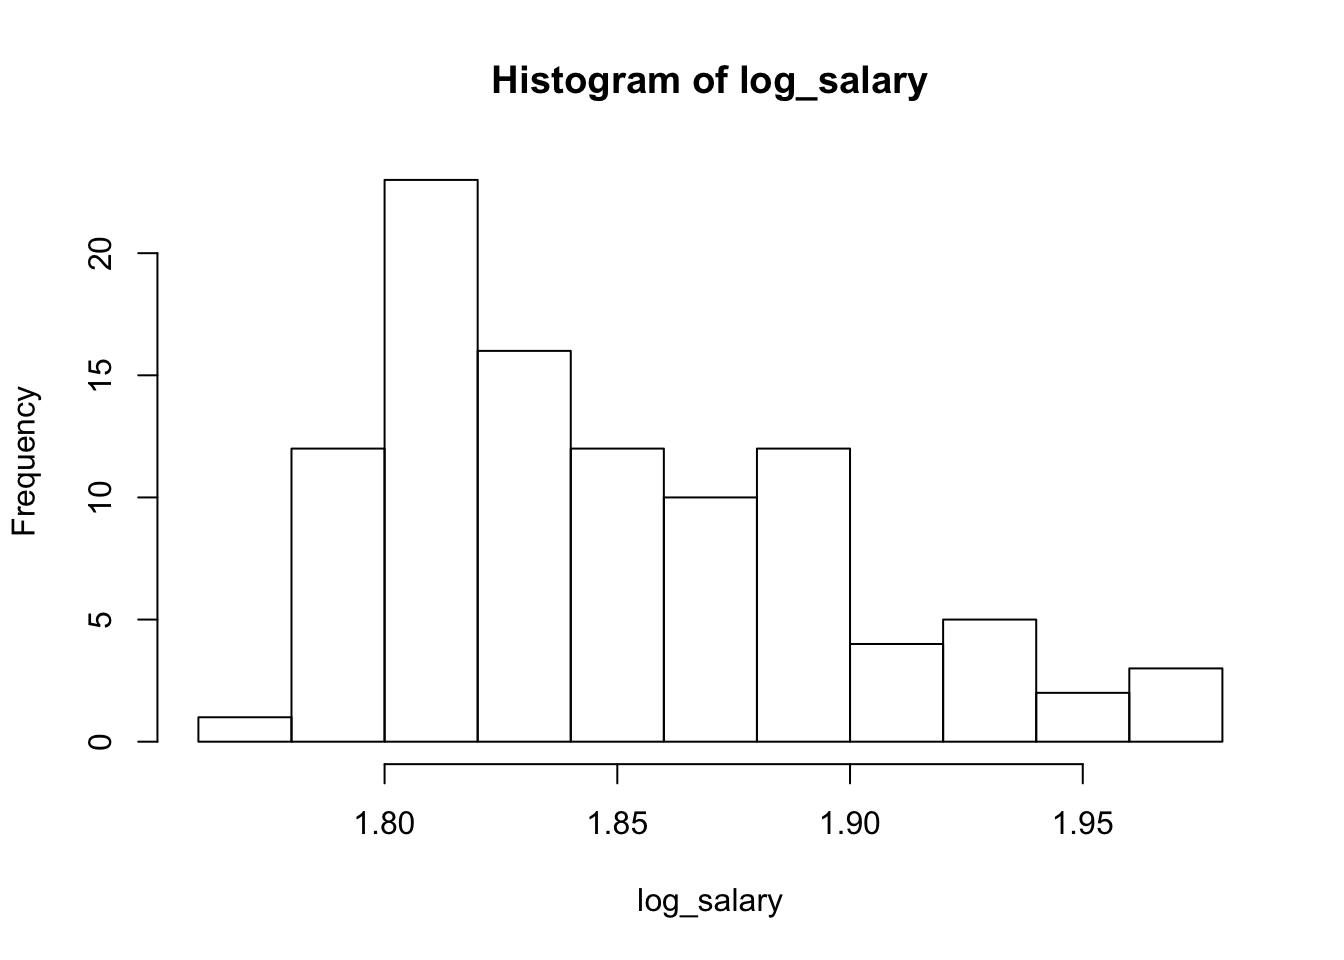
\includegraphics{tsAssignment03_files/figure-latex/unnamed-chunk-2-1.pdf}

\begin{Shaded}
\begin{Highlighting}[]
\KeywordTok{residual.analysis}\NormalTok{(}
\NormalTok{  model_linear, }
  \DataTypeTok{std =} \OtherTok{TRUE}\NormalTok{, }
  \DataTypeTok{start =} \DecValTok{1}\NormalTok{,   }
  \DataTypeTok{title =} \KeywordTok{fig_nums}\NormalTok{(}\StringTok{'linear_residual'}\NormalTok{, }\StringTok{'Linear model residual analysis'}\NormalTok{)}
\NormalTok{)}
\end{Highlighting}
\end{Shaded}

\begin{verbatim}
## 
##  Shapiro-Wilk normality test
## 
## data:  res.model
## W = 0.82362, p-value < 2.2e-16
\end{verbatim}

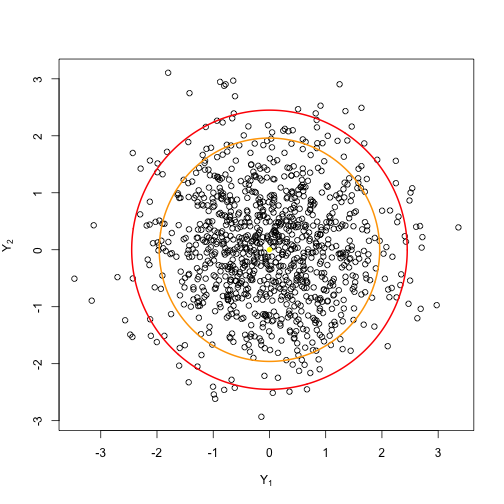
\includegraphics{tsAssignment03_files/figure-latex/unnamed-chunk-3-1.pdf}

\begin{Shaded}
\begin{Highlighting}[]
\CommentTok{# fitted values}
\CommentTok{# add dates}
\NormalTok{forecastDatesRange <-}\StringTok{ }\KeywordTok{data.frame}\NormalTok{(}\DataTypeTok{time =} \KeywordTok{seq}\NormalTok{(}\KeywordTok{as.Date}\NormalTok{(}\StringTok{'2019-2-25'}\NormalTok{), }\KeywordTok{as.Date}\NormalTok{(}\StringTok{'2019-3-6'}\NormalTok{), }\DataTypeTok{by =} \StringTok{"day"}\NormalTok{))}
\CommentTok{# convert dates to numeric}
\NormalTok{numericDates <-}\StringTok{ }\KeywordTok{ts}\NormalTok{(}
  \KeywordTok{as.vector}\NormalTok{(forecastDatesRange),  }
  \DataTypeTok{start =}\NormalTok{ startForecast, }
  \DataTypeTok{frequency =}\NormalTok{ frequency)}
\CommentTok{# ensure data has the same label (time)}
\NormalTok{time =}\StringTok{ }\KeywordTok{time}\NormalTok{(numericDates)}
\NormalTok{timeDataFrame =}\StringTok{ }\KeywordTok{data.frame}\NormalTok{(time)}
\CommentTok{# prediction}
\NormalTok{forecastLinear =}\StringTok{ }\KeywordTok{predict.lm}\NormalTok{(model_linear, timeDataFrame, }\DataTypeTok{interval =} \StringTok{"prediction"}\NormalTok{)}
\KeywordTok{print}\NormalTok{(forecastLinear)}
\end{Highlighting}
\end{Shaded}

\begin{verbatim}
##         fit      lwr      upr
## 1  6377.077 1545.802 11208.35
## 2  6380.855 1549.573 11212.14
## 3  6384.633 1553.345 11215.92
## 4  6388.411 1557.117 11219.70
## 5  6392.189 1560.889 11223.49
## 6  6395.967 1564.660 11227.27
## 7  6399.745 1568.432 11231.06
## 8  6403.523 1572.204 11234.84
## 9  6407.302 1575.975 11238.63
## 10 6411.080 1579.747 11242.41
\end{verbatim}

\begin{Shaded}
\begin{Highlighting}[]
\CommentTok{# convert prediction back to ts object}
\NormalTok{linear_predict =}\StringTok{ }\KeywordTok{ts}\NormalTok{(}
\NormalTok{  forecastLinear[,}\DecValTok{1}\NormalTok{],}
  \DataTypeTok{start =}\NormalTok{ startForecast,}
  \DataTypeTok{frequency =}\NormalTok{ frequency}
\NormalTok{)}
\end{Highlighting}
\end{Shaded}

\begin{Shaded}
\begin{Highlighting}[]
\CommentTok{# calculate MASE with observed and predicted values}
\KeywordTok{MASE}\NormalTok{(real.ts, linear_predict)}
\end{Highlighting}
\end{Shaded}

\begin{verbatim}
## $MASE
##      MASE
## 1 78.6479
\end{verbatim}

\begin{Shaded}
\begin{Highlighting}[]
\CommentTok{# plot }
\KeywordTok{doPar}\NormalTok{(}\KeywordTok{c}\NormalTok{(}\DecValTok{2}\NormalTok{,}\DecValTok{1}\NormalTok{))}
\KeywordTok{plot}\NormalTok{(data.ts)}
\KeywordTok{lines}\NormalTok{(real.ts, }\DataTypeTok{col =} \StringTok{"red"}\NormalTok{)}
\KeywordTok{lines}\NormalTok{(linear_predict, }\DataTypeTok{col=}\StringTok{"red"}\NormalTok{, }\DataTypeTok{type=}\StringTok{"l"}\NormalTok{)}
\KeywordTok{zoomplot.zoom}\NormalTok{(}\DataTypeTok{xlim=}\KeywordTok{c}\NormalTok{(}\FloatTok{2019.1}\NormalTok{,}\FloatTok{2019.3}\NormalTok{))}
\end{Highlighting}
\end{Shaded}

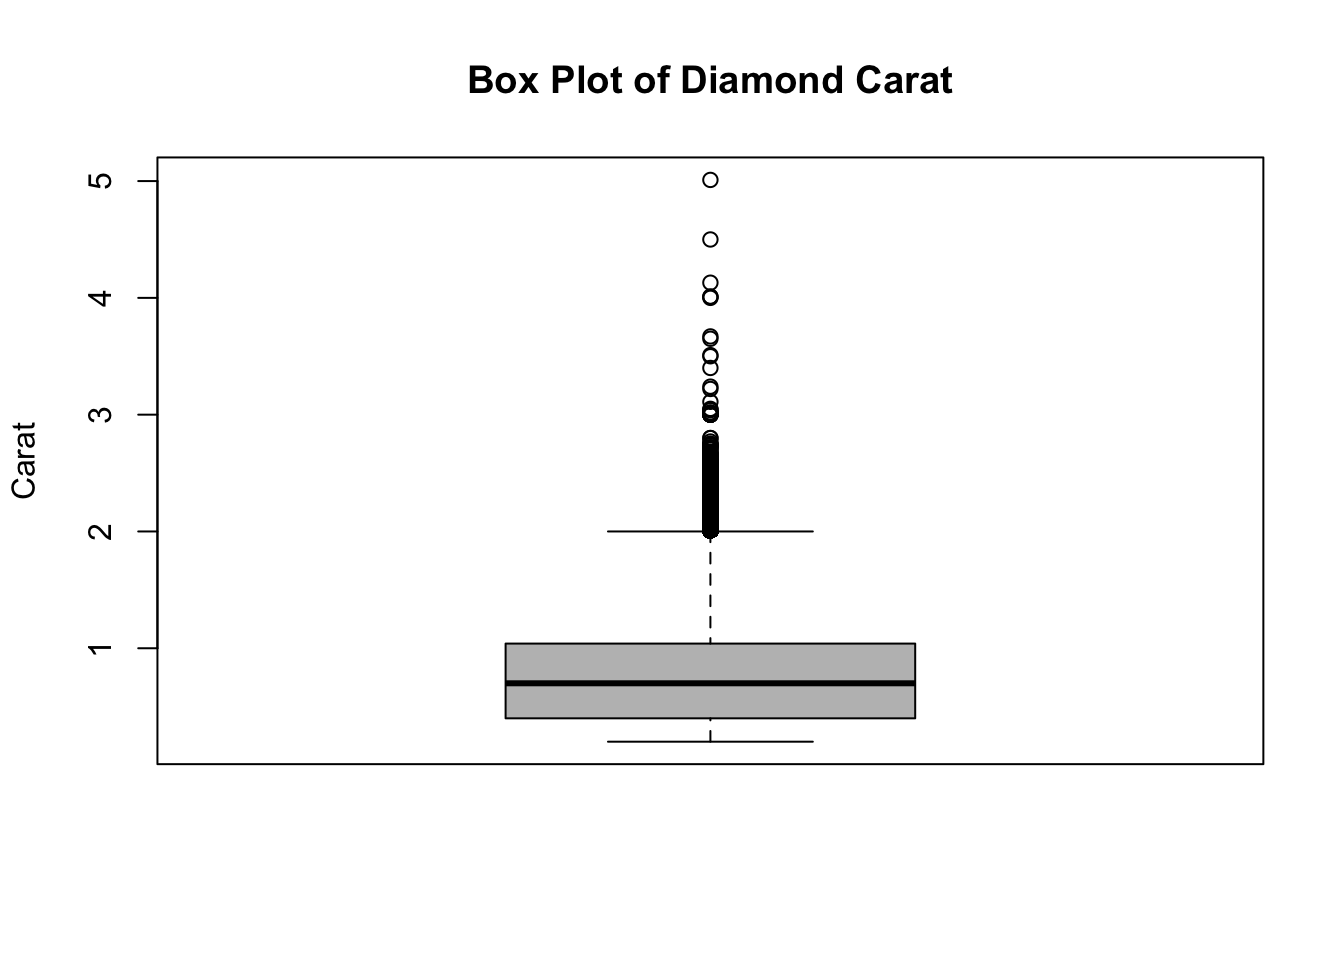
\includegraphics{tsAssignment03_files/figure-latex/unnamed-chunk-4-1.pdf}

\begin{itemize}
\tightlist
\item
  The standardised residuals are not white noise and show that the model
  has not captured the trend of the data
\item
  histogram: left skewed
\item
  Ljung-Box test: all lags are significant
\item
  Q-Q plot: left-tailed, doesn't fit along one line, therefore not
  normally distributed
\item
  ACF: there are significant lags which does not fit with a white noise
  series
\item
  Shapiro-Wilk: significant, therefore reject the null that the
  residuals are normally distributed
\item
  TODO: comment on predicted values
\end{itemize}

\hypertarget{quadratic-model}{%
\subsection{Quadratic Model}\label{quadratic-model}}

\begin{Shaded}
\begin{Highlighting}[]
\NormalTok{time =}\StringTok{ }\KeywordTok{time}\NormalTok{(data.ts)}
\NormalTok{time2 =}\StringTok{ }\NormalTok{time }\OperatorTok{^}\StringTok{ }\DecValTok{2}
\NormalTok{model_quadratic =}\StringTok{ }\KeywordTok{lm}\NormalTok{(data.ts }\OperatorTok{~}\StringTok{ }\NormalTok{time }\OperatorTok{+}\StringTok{ }\NormalTok{time2) }\CommentTok{# label the quadratic trend model}
\KeywordTok{summary}\NormalTok{(model_quadratic)}
\end{Highlighting}
\end{Shaded}

\begin{verbatim}
## 
## Call:
## lm(formula = data.ts ~ time + time2)
## 
## Residuals:
##     Min      1Q  Median      3Q     Max 
## -5044.0  -942.0  -196.7   435.7 14722.9 
## 
## Coefficients:
##               Estimate Std. Error t value Pr(>|t|)    
## (Intercept)  1.608e+09  7.809e+07   20.59   <2e-16 ***
## time        -1.597e+06  7.746e+04  -20.61   <2e-16 ***
## time2        3.963e+02  1.921e+01   20.63   <2e-16 ***
## ---
## Signif. codes:  0 '***' 0.001 '**' 0.01 '*' 0.05 '.' 0.1 ' ' 1
## 
## Residual standard error: 2247 on 2127 degrees of freedom
## Multiple R-squared:  0.5595, Adjusted R-squared:  0.5591 
## F-statistic:  1351 on 2 and 2127 DF,  p-value: < 2.2e-16
\end{verbatim}

\begin{Shaded}
\begin{Highlighting}[]
\KeywordTok{doPar}\NormalTok{(}\DataTypeTok{mfrow =} \KeywordTok{c}\NormalTok{(}\DecValTok{1}\NormalTok{, }\DecValTok{1}\NormalTok{))}
\KeywordTok{plot}\NormalTok{(}
  \KeywordTok{ts}\NormalTok{(}\KeywordTok{fitted}\NormalTok{(model_quadratic)),}
  \DataTypeTok{ylim =} \KeywordTok{c}\NormalTok{(}\KeywordTok{min}\NormalTok{(}\KeywordTok{c}\NormalTok{(}
    \KeywordTok{fitted}\NormalTok{(model_quadratic), }\KeywordTok{as.vector}\NormalTok{(data.ts)}
\NormalTok{  )),}
  \KeywordTok{max}\NormalTok{(}\KeywordTok{c}\NormalTok{(}
    \KeywordTok{fitted}\NormalTok{(model_quadratic), }\KeywordTok{as.vector}\NormalTok{(data.ts)}
\NormalTok{  ))),}
  \DataTypeTok{ylab =}\NormalTok{ default_ylab,}
  \DataTypeTok{main =} \KeywordTok{fig_nums}\NormalTok{(}
    \StringTok{"quadratic_model"}\NormalTok{,}
    \StringTok{"Bitcoin Data with Quadratic Model"}\NormalTok{)}
\NormalTok{)}
\KeywordTok{lines}\NormalTok{(}\KeywordTok{as.vector}\NormalTok{(data.ts))}
\end{Highlighting}
\end{Shaded}

\includegraphics{tsAssignment03_files/figure-latex/unnamed-chunk-5-1.pdf}

\begin{Shaded}
\begin{Highlighting}[]
\NormalTok{newdata <-}\StringTok{ }\KeywordTok{data.frame}\NormalTok{(}\DataTypeTok{time =} \KeywordTok{seq}\NormalTok{(}\KeywordTok{as.Date}\NormalTok{(}\StringTok{'2019-2-25'}\NormalTok{), }\KeywordTok{as.Date}\NormalTok{(}\StringTok{'2019-3-6'}\NormalTok{), }\DataTypeTok{by =} \StringTok{"day"}\NormalTok{))}
\NormalTok{newdata1 <-}\StringTok{ }\KeywordTok{ts}\NormalTok{(}\KeywordTok{as.vector}\NormalTok{(newdata),}\DataTypeTok{start =} \KeywordTok{c}\NormalTok{(}\DecValTok{2019}\NormalTok{,}\KeywordTok{as.numeric}\NormalTok{(}\KeywordTok{format}\NormalTok{(inds[}\DecValTok{1}\NormalTok{], }\StringTok{"%j"}\NormalTok{))), }\DataTypeTok{frequency =} \FloatTok{365.25}\NormalTok{)}

\KeywordTok{residual.analysis}\NormalTok{(}
\NormalTok{  model_quadratic, }\DataTypeTok{std =} \OtherTok{TRUE}\NormalTok{, }\DataTypeTok{start =} \DecValTok{1}\NormalTok{,}
  \DataTypeTok{title =} \KeywordTok{fig_nums}\NormalTok{(}
    \StringTok{'quadratic_model_residual'}\NormalTok{, }
    \StringTok{'Quadratic model residual analysis'}\NormalTok{))}
\end{Highlighting}
\end{Shaded}

\begin{verbatim}
## 
##  Shapiro-Wilk normality test
## 
## data:  res.model
## W = 0.74654, p-value < 2.2e-16
\end{verbatim}

\begin{verbatim}
## Warning in (ra^2)/(n - (1:lag.max)): longer object length is not a multiple
## of shorter object length
\end{verbatim}

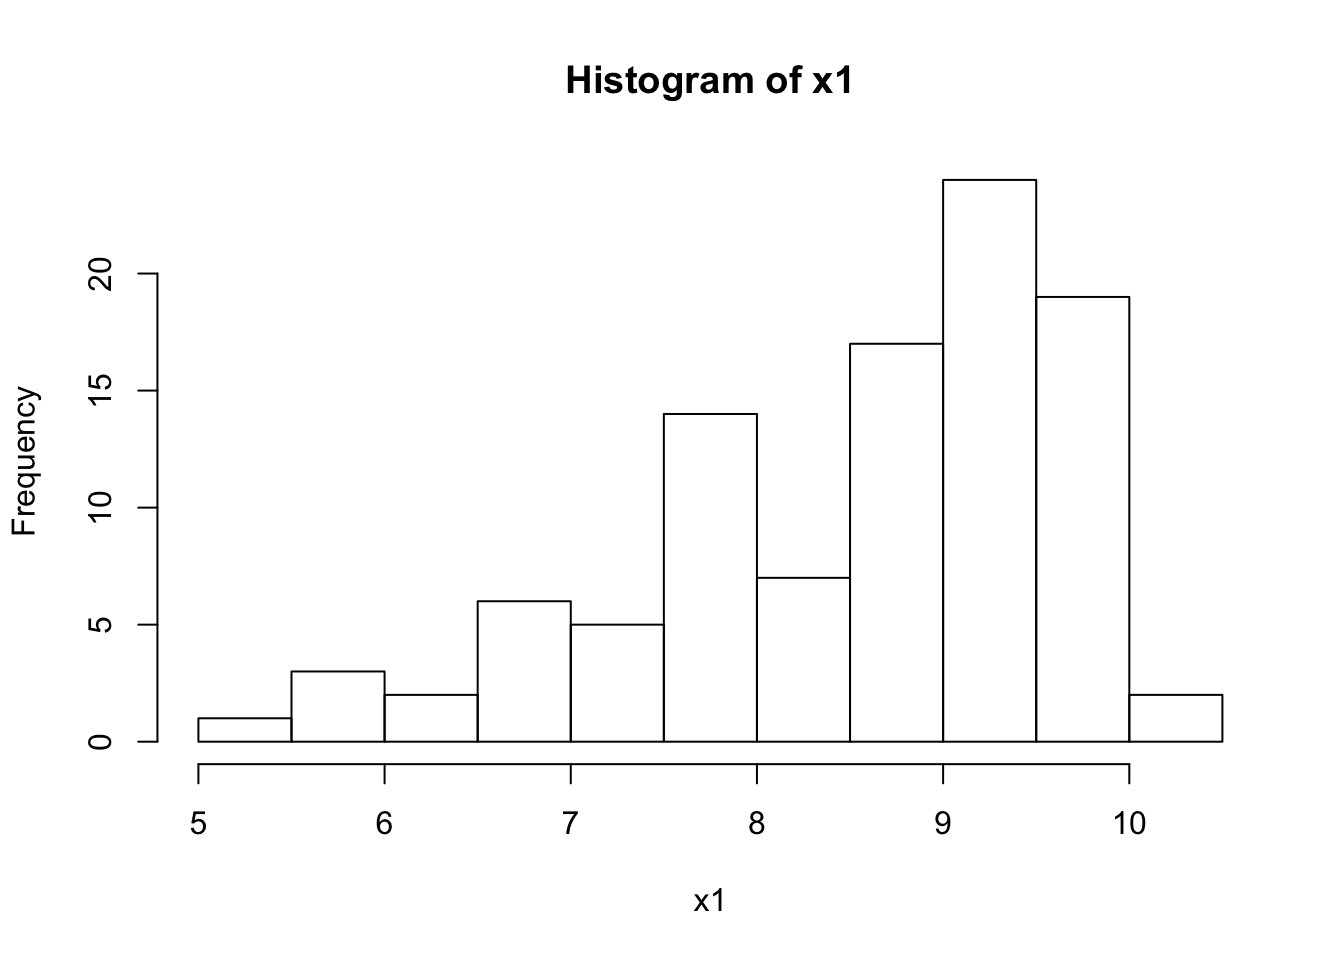
\includegraphics{tsAssignment03_files/figure-latex/unnamed-chunk-6-1.pdf}

\begin{Shaded}
\begin{Highlighting}[]
\CommentTok{# predict}
\NormalTok{time =}\StringTok{ }\KeywordTok{time}\NormalTok{(newdata1)}
\NormalTok{time2 =}\StringTok{ }\NormalTok{time}\OperatorTok{^}\DecValTok{2}
\NormalTok{newdata3 =}\StringTok{ }\KeywordTok{data.frame}\NormalTok{(time,time2)}
\NormalTok{forecastQuadratic =}\StringTok{ }\KeywordTok{predict}\NormalTok{(model_quadratic, newdata3, }\DataTypeTok{interval =} \StringTok{"prediction"}\NormalTok{)}
\KeywordTok{print}\NormalTok{(forecastQuadratic)}
\end{Highlighting}
\end{Shaded}

\begin{verbatim}
##         fit      lwr      upr
## 1  9257.384 4838.611 13676.16
## 2  9267.860 4849.045 13686.68
## 3  9278.343 4859.485 13697.20
## 4  9288.831 4869.931 13707.73
## 5  9299.326 4880.382 13718.27
## 6  9309.826 4890.840 13728.81
## 7  9320.332 4901.303 13739.36
## 8  9330.844 4911.772 13749.92
## 9  9341.363 4922.246 13760.48
## 10 9351.887 4932.727 13771.05
\end{verbatim}

\begin{Shaded}
\begin{Highlighting}[]
\NormalTok{quadratic_predict =}\StringTok{ }\KeywordTok{ts}\NormalTok{(forecastQuadratic[,}\DecValTok{1}\NormalTok{], }
  \DataTypeTok{start =} \KeywordTok{c}\NormalTok{(}\DecValTok{2019}\NormalTok{, }\KeywordTok{as.numeric}\NormalTok{(}\KeywordTok{format}\NormalTok{(inds[}\DecValTok{1}\NormalTok{], }\StringTok{"%j"}\NormalTok{))),}
  \DataTypeTok{frequency =} \FloatTok{365.25}\NormalTok{)}

\KeywordTok{MASE}\NormalTok{(real.ts, quadratic_predict)}
\end{Highlighting}
\end{Shaded}

\begin{verbatim}
## Warning in .cbind.ts(list(e1, e2), c(deparse(substitute(e1))[1L],
## deparse(substitute(e2))[1L]), : non-intersecting series
\end{verbatim}

\begin{verbatim}
## $MASE
##   MASE
## 1  NaN
\end{verbatim}

\begin{itemize}
\tightlist
\item
  The residuals are largely unchanged from the linear plot
\item
  The standardised residuals are not white noise and show that the model
  has not captured the trend of the data
\item
  histogram: left skewed
\item
  Ljung-Box test: all lags are significant
\item
  Q-Q plot: left-tailed, doesn't fit along one line, therefore not
  normally distributed
\item
  ACF: there are significant lags which does not fit with a white noise
  series
\item
  Shapiro-Wilk: significant, therefore reject the null that the
  residuals are normally distributed
\item
  TODO: comment on predicted values/MASE
\end{itemize}

\begin{Shaded}
\begin{Highlighting}[]
\KeywordTok{doDiffAndPlot}\NormalTok{(data.ts, }\DecValTok{0}\NormalTok{, T, T, }\StringTok{'Bitcoin diff=0'}\NormalTok{)}
\end{Highlighting}
\end{Shaded}

\begin{verbatim}
## diff:  0 
## 
## 
## adf p-value: 
## > 0.05 insignificant
##  0.216405558751826
\end{verbatim}

\includegraphics{tsAssignment03_files/figure-latex/plot-no-diff-1.pdf}

\begin{itemize}
\item
  acf plot slowly decaying lags i.e.~not stationary
\item
  the adf test confirms that the series is not stationary
\item
  the series will be transformed and/or differenced before fitting ARIMA
\item
  Therefore: we will transform the data with log or Box Cox
\end{itemize}

\hypertarget{confidence-interval-of-lambda}{%
\subsubsection{Confidence interval of
Lambda}\label{confidence-interval-of-lambda}}

\begin{Shaded}
\begin{Highlighting}[]
\CommentTok{# check the confidence interval of lambda}
\CommentTok{# }\AlertTok{TODO}\CommentTok{: half-sized version of this plot}
\KeywordTok{doPar}\NormalTok{(}\DataTypeTok{mfrow =} \KeywordTok{c}\NormalTok{(}\DecValTok{1}\NormalTok{,}\DecValTok{1}\NormalTok{))}
\NormalTok{boxcoxCi <-}\StringTok{ }\KeywordTok{BoxCox.ar}\NormalTok{(data.ts, }\DataTypeTok{method =} \StringTok{"yule-walker"}\NormalTok{)}\OperatorTok{$}\NormalTok{ci}
\NormalTok{boxcoxCi}
\end{Highlighting}
\end{Shaded}

\begin{verbatim}
## [1] 0 0
\end{verbatim}

\begin{Shaded}
\begin{Highlighting}[]
\KeywordTok{title}\NormalTok{(}\KeywordTok{fig_nums}\NormalTok{(}\StringTok{'boxcox_ci'}\NormalTok{,}\StringTok{'Confidence Interval of Lambda of Bitcoin'}\NormalTok{), }\DataTypeTok{line =} \FloatTok{-1.5}\NormalTok{, }\DataTypeTok{outer =} \OtherTok{TRUE}\NormalTok{)}
\end{Highlighting}
\end{Shaded}

\includegraphics{tsAssignment03_files/figure-latex/confidence-interval-1.pdf}

lambda == 0

\begin{itemize}
\tightlist
\item
  The confidence interval does include 0, so we \emph{will} do a log
  transform
\end{itemize}

\hypertarget{log-transform}{%
\subsection{Log Transform}\label{log-transform}}

\begin{Shaded}
\begin{Highlighting}[]
\NormalTok{data.ts__log =}\StringTok{ }\KeywordTok{log}\NormalTok{(data.ts)}
\KeywordTok{doDiffAndPlot}\NormalTok{(}
\NormalTok{  data.ts__log, }\DecValTok{0}\NormalTok{, T, T,}
  \KeywordTok{fig_nums}\NormalTok{(}\StringTok{"log_transform"}\NormalTok{, }\StringTok{"Log transform"}\NormalTok{))}
\end{Highlighting}
\end{Shaded}

\begin{verbatim}
## diff:  0 
## 
## 
## adf p-value: 
## > 0.05 insignificant
##  0.923249395126087
\end{verbatim}

\includegraphics{tsAssignment03_files/figure-latex/log_transform-1.pdf}

\begin{itemize}
\tightlist
\item
  the adf test p-value is not significant meaning the series is not
  stationary
\item
  acf still has the same pattern
\end{itemize}

\hypertarget{log-first-diff}{%
\subsubsection{Log first diff}\label{log-first-diff}}

\begin{Shaded}
\begin{Highlighting}[]
\KeywordTok{doDiffAndPlot}\NormalTok{(}
\NormalTok{  data.ts__log, }\DecValTok{1}\NormalTok{, T, T,}
  \KeywordTok{fig_nums}\NormalTok{(}\StringTok{'log_first_diff'}\NormalTok{, }\StringTok{'Log first diff'}\NormalTok{))}
\end{Highlighting}
\end{Shaded}

\begin{verbatim}
## diff:  1
\end{verbatim}

\begin{verbatim}
## Warning in adfTest(df.ts, lags = order, title = NULL, description = NULL):
## p-value smaller than printed p-value
\end{verbatim}

\begin{verbatim}
## 
## adf p-value: 
## 0.01 < 0.05 significant
## 
## AR/MA
##   0 1 2 3 4 5 6 7 8 9 10 11 12 13
## 0 o o o o x x o o o x x  o  o  o 
## 1 x o o o o x o o o o x  o  o  o 
## 2 o x o o o x o o o o x  o  o  o 
## 3 o x o o o x o o o o x  o  o  o 
## 4 x x o x o x o o o o x  o  o  o 
## 5 x x x x x o o o o o x  o  o  o 
## 6 x x x x x o o o o o o  o  o  o 
## 7 x x o x x x x o o o o  o  o  o
\end{verbatim}

\includegraphics{tsAssignment03_files/figure-latex/log-first-diff-1.pdf}

\begin{Shaded}
\begin{Highlighting}[]
\NormalTok{data.ts__log_diff1 =}\StringTok{ }\NormalTok{data.ts__log }\OperatorTok\StringTok{ }\KeywordTok{diff}\NormalTok{(}\DataTypeTok{differences =} \DecValTok{1}\NormalTok{)}
\end{Highlighting}
\end{Shaded}

\begin{itemize}
\item
  the adf test p-value is significant - therefore the series is now
  stationary
\item
  However, doesn't have constant variance - an assumption for ARIMA
  models
\item
  there are many significant serial correlations in the data which
  suggests that the data exhibits serial dependence
\item
  Based on EACF plot, we can add the following models:
  \texttt{\{ARIMA(0,1,1),\ ARIMA(1,1,1)\}}
\end{itemize}

\hypertarget{log-second-diff}{%
\subsubsection{Log Second diff}\label{log-second-diff}}

Although we have a significant adf value \texttt{(p\ \textless{}\ 0.05)}
for log first diff, we will overdifference with \texttt{d\ =\ 2} because
of the high number of lags in both the ACF and PACF

\begin{Shaded}
\begin{Highlighting}[]
\KeywordTok{doDiffAndPlot}\NormalTok{(data.ts__log, }\DecValTok{2}\NormalTok{, T, T,}
  \DataTypeTok{plotTitle =} \KeywordTok{fig_nums}\NormalTok{(}\StringTok{'log_second_diff'}\NormalTok{, }\StringTok{'Log second diff'}\NormalTok{))}
\end{Highlighting}
\end{Shaded}

\begin{verbatim}
## diff:  2
\end{verbatim}

\begin{verbatim}
## Warning in adfTest(df.ts, lags = order, title = NULL, description = NULL):
## p-value smaller than printed p-value
\end{verbatim}

\begin{verbatim}
## 
## adf p-value: 
## 0.01 < 0.05 significant
## 
## AR/MA
##   0 1 2 3 4 5 6 7 8 9 10 11 12 13
## 0 x o o o o x x o o o x  o  o  o 
## 1 x x o o o x x o o o x  o  x  o 
## 2 x x o o o x x x o o x  o  o  o 
## 3 x x o o o x o o o o x  o  o  o 
## 4 x o o o x o o o o o o  o  o  o 
## 5 x x x x x o o o o o o  o  o  o 
## 6 x o x x x x x o o o o  o  o  o 
## 7 x o x x x x x x o o o  o  o  o
\end{verbatim}

\includegraphics{tsAssignment03_files/figure-latex/log-second-diff-1.pdf}

\begin{Shaded}
\begin{Highlighting}[]
\NormalTok{data.ts__log_diff2 =}\StringTok{ }\NormalTok{data.ts__log }\OperatorTok\StringTok{ }\KeywordTok{diff}\NormalTok{(}\DataTypeTok{differences =} \DecValTok{2}\NormalTok{)}
\end{Highlighting}
\end{Shaded}

\begin{itemize}
\tightlist
\item
  Success of a single MA lag
\item
  Problem of more than 10 significant lags in AR
\item
  Based on EACF plot, we can add the following models:
  \texttt{\{ARIMA(0,2,1),\ ARIMA(0,2,2),\ ARIMA(1,2,2)\}}
\end{itemize}

\hypertarget{get-possible-models-formula}{%
\subsubsection{Get possible models
formula}\label{get-possible-models-formula}}

\begin{Shaded}
\begin{Highlighting}[]
\KeywordTok{findBestModel}\NormalTok{(data.ts__log)}
\end{Highlighting}
\end{Shaded}

\begin{verbatim}
## | AIC | Order | Shapiro Residuals p-value | 
##  | --------- | ---------- | --------------------- |
## | -7302.399 | 0 1 0 | 3.882959e-37 | 
## | -7300.42 | 1 1 0 | 3.985837e-37 | 
## | -7299.027 | 2 1 0 | 3.77238e-37 | 
## | -7300.421 | 0 1 1 | 3.989343e-37 | 
## | -7298.421 | 1 1 1 | 3.987566e-37 | 
## | -7297.027 | 2 1 1 | 3.771705e-37 | 
## | -7299 | 0 1 2 | 3.777204e-37 | 
## | -7296.999 | 1 1 2 | 3.77752e-37 | 
## | -7324 | 2 1 2 | 3.183622e-36 | 
## | -5835.035 | 0 2 0 | 7.008529e-36 | 
## | -6415.021 | 1 2 0 | 4.32332e-35 | 
## | -6674.674 | 2 2 0 | 8.092037e-36 | 
## | -7291.597 | 0 2 1 | 2.490153e-37 | 
## | -7289.602 | 1 2 1 | 2.450695e-37 | 
## | -7288.64 | 2 2 1 | 2.125636e-37 | 
## | -7289.602 | 0 2 2 | 2.445985e-37 | 
## | -7287.651 | 1 2 2 | 2.572079e-37 | 
## | -7286.404 | 2 2 2 | 2.139399e-37 |
\end{verbatim}

It isn't obvious whether we should use \texttt{diff\ =\ 1}, or
\texttt{diff\ =\ 2} moving forward. So, we wrote a small function to
loop to find the best possible ARIMA models based on AIC with the
\texttt{method=CSS-ML}

Please note: - \texttt{\{ARIMA(0,1,0)\ and\ ARIMA(0,2,0)\}} are not
useful models, so we will ignore them

\hypertarget{list-of-possible-models-ordered-by-aic}{%
\paragraph{List of possible models ordered by
AIC:}\label{list-of-possible-models-ordered-by-aic}}

\begin{longtable}[]{@{}lll@{}}
\toprule
AIC & Order & Shapiro Residuals p-value\tabularnewline
\midrule
\endhead
-7324 & 2 1 2 & 3.183622e-36\tabularnewline
-7302.399 & 0 1 0 & 3.882959e-37\tabularnewline
-7300.421 & 0 1 1 & 3.989343e-37\tabularnewline
-7300.42 & 1 1 0 & 3.985837e-37\tabularnewline
-7299.027 & 2 1 0 & 3.77238e-37\tabularnewline
-7299 & 0 1 2 & 3.777204e-37\tabularnewline
-7298.421 & 1 1 1 & 3.987566e-37\tabularnewline
-7297.027 & 2 1 1 & 3.771705e-37\tabularnewline
-7296.999 & 1 1 2 & 3.77752e-37\tabularnewline
-7291.597 & 0 2 1 & 2.490153e-37\tabularnewline
-7289.602 & 1 2 1 & 2.450695e-37\tabularnewline
-7289.602 & 0 2 2 & 2.445985e-37\tabularnewline
-7288.64 & 2 2 1 & 2.125636e-37\tabularnewline
-7287.651 & 1 2 2 & 2.572079e-37\tabularnewline
-7286.404 & 2 2 2 & 2.139399e-37\tabularnewline
-6674.674 & 2 2 0 & 8.092037e-36\tabularnewline
-6415.021 & 1 2 0 & 4.32332e-35\tabularnewline
-5835.035 & 0 2 0 & 7.008529e-36\tabularnewline
\bottomrule
\end{longtable}

Moving forward, we will select the following models: - because we want
the
\href{https://stats.stackexchange.com/questions/84076/negative-values-for-aic-in-general-mixed-model}{lowest
possible AIC value} - we ignore all diff= 2 because of the obvious AIC
score being lower for all

\hypertarget{final-set-of-candidate-models}{%
\subsubsection{Final set of candidate
models:}\label{final-set-of-candidate-models}}

\begin{longtable}[]{@{}lll@{}}
\toprule
AIC & Order & Shapiro Residuals p-value\tabularnewline
\midrule
\endhead
-7324 & 2 1 2 & 3.183622e-36\tabularnewline
-7300.421 & 0 1 1 & 3.989343e-37\tabularnewline
-7300.42 & 1 1 0 & 3.985837e-37\tabularnewline
-7299.027 & 2 1 0 & 3.77238e-37\tabularnewline
-7299 & 0 1 2 & 3.777204e-37\tabularnewline
-7298.421 & 1 1 1 & 3.987566e-37\tabularnewline
-7297.027 & 2 1 1 & 3.771705e-37\tabularnewline
-7296.999 & 1 1 2 & 3.77752e-37\tabularnewline
\bottomrule
\end{longtable}

\begin{Shaded}
\begin{Highlighting}[]
\NormalTok{possibleArimaModels <-}\StringTok{ }\KeywordTok{list}\NormalTok{()}
\NormalTok{newArima <-}
\StringTok{  }\KeywordTok{list}\NormalTok{(  }
    \KeywordTok{c}\NormalTok{(}\DecValTok{2}\NormalTok{, }\DecValTok{1}\NormalTok{, }\DecValTok{2}\NormalTok{),   }\CommentTok{# arima(2, 1, 2)}
    \KeywordTok{c}\NormalTok{(}\DecValTok{0}\NormalTok{, }\DecValTok{1}\NormalTok{, }\DecValTok{1}\NormalTok{),   }\CommentTok{# arima(0, 1, 1)}
    \KeywordTok{c}\NormalTok{(}\DecValTok{1}\NormalTok{, }\DecValTok{1}\NormalTok{, }\DecValTok{0}\NormalTok{),   }\CommentTok{# arima(1, 1, 0)}
    \KeywordTok{c}\NormalTok{(}\DecValTok{2}\NormalTok{, }\DecValTok{1}\NormalTok{, }\DecValTok{0}\NormalTok{),   }\CommentTok{# arima(2, 1, 0)}
    \KeywordTok{c}\NormalTok{(}\DecValTok{0}\NormalTok{, }\DecValTok{1}\NormalTok{, }\DecValTok{2}\NormalTok{),   }\CommentTok{# arima(0, 1, 2)}
    \KeywordTok{c}\NormalTok{(}\DecValTok{1}\NormalTok{, }\DecValTok{1}\NormalTok{, }\DecValTok{1}\NormalTok{),   }\CommentTok{# arima(1, 1, 1)}
    \KeywordTok{c}\NormalTok{(}\DecValTok{2}\NormalTok{, }\DecValTok{1}\NormalTok{, }\DecValTok{1}\NormalTok{),   }\CommentTok{# arima(2, 1, 1)}
    \KeywordTok{c}\NormalTok{(}\DecValTok{1}\NormalTok{, }\DecValTok{1}\NormalTok{, }\DecValTok{2}\NormalTok{)   }\CommentTok{# arima(1, 1, 2)}
\NormalTok{  )}
\NormalTok{possibleArimaModels <-}\StringTok{ }\KeywordTok{c}\NormalTok{(possibleArimaModels, newArima) }
\end{Highlighting}
\end{Shaded}

\hypertarget{estimation-of-parameters}{%
\subsection{Estimation of Parameters}\label{estimation-of-parameters}}

\hypertarget{arima}{%
\subsubsection{ARIMA}\label{arima}}

\begin{Shaded}
\begin{Highlighting}[]
\CommentTok{# possibleArimaModels}
\NormalTok{model_}\DecValTok{212}\NormalTok{_ml <-}\StringTok{ }\KeywordTok{arima}\NormalTok{(data.ts__log_diff1, }\KeywordTok{c}\NormalTok{(}\DecValTok{2}\NormalTok{,}\DecValTok{0}\NormalTok{,}\DecValTok{2}\NormalTok{), }\DataTypeTok{method=}\StringTok{'ML'}\NormalTok{)}
\end{Highlighting}
\end{Shaded}

\begin{verbatim}
## Warning in stats::arima(x = x, order = order, seasonal = seasonal, xreg =
## xreg, : possible convergence problem: optim gave code = 1
\end{verbatim}

\begin{Shaded}
\begin{Highlighting}[]
\NormalTok{model_}\DecValTok{011}\NormalTok{_ml <-}\StringTok{ }\KeywordTok{arima}\NormalTok{(data.ts__log_diff1, }\KeywordTok{c}\NormalTok{(}\DecValTok{0}\NormalTok{,}\DecValTok{0}\NormalTok{,}\DecValTok{1}\NormalTok{), }\DataTypeTok{method=}\StringTok{'ML'}\NormalTok{)}
\NormalTok{model_}\DecValTok{110}\NormalTok{_ml <-}\StringTok{ }\KeywordTok{arima}\NormalTok{(data.ts__log_diff1, }\KeywordTok{c}\NormalTok{(}\DecValTok{1}\NormalTok{,}\DecValTok{0}\NormalTok{,}\DecValTok{0}\NormalTok{), }\DataTypeTok{method=}\StringTok{'ML'}\NormalTok{)}
\NormalTok{model_}\DecValTok{210}\NormalTok{_ml <-}\StringTok{ }\KeywordTok{arima}\NormalTok{(data.ts__log_diff1, }\KeywordTok{c}\NormalTok{(}\DecValTok{2}\NormalTok{,}\DecValTok{0}\NormalTok{,}\DecValTok{0}\NormalTok{), }\DataTypeTok{method=}\StringTok{'ML'}\NormalTok{)}
\NormalTok{model_}\DecValTok{012}\NormalTok{_ml <-}\StringTok{ }\KeywordTok{arima}\NormalTok{(data.ts__log_diff1, }\KeywordTok{c}\NormalTok{(}\DecValTok{0}\NormalTok{,}\DecValTok{0}\NormalTok{,}\DecValTok{2}\NormalTok{), }\DataTypeTok{method=}\StringTok{'ML'}\NormalTok{)}
\NormalTok{model_}\DecValTok{111}\NormalTok{_ml <-}\StringTok{ }\KeywordTok{arima}\NormalTok{(data.ts__log_diff1, }\KeywordTok{c}\NormalTok{(}\DecValTok{1}\NormalTok{,}\DecValTok{0}\NormalTok{,}\DecValTok{1}\NormalTok{), }\DataTypeTok{method=}\StringTok{'ML'}\NormalTok{)}
\NormalTok{model_}\DecValTok{211}\NormalTok{_ml <-}\StringTok{ }\KeywordTok{arima}\NormalTok{(data.ts__log_diff1, }\KeywordTok{c}\NormalTok{(}\DecValTok{2}\NormalTok{,}\DecValTok{0}\NormalTok{,}\DecValTok{1}\NormalTok{), }\DataTypeTok{method=}\StringTok{'ML'}\NormalTok{)}
\NormalTok{model_}\DecValTok{112}\NormalTok{_ml <-}\StringTok{ }\KeywordTok{arima}\NormalTok{(data.ts__log_diff1, }\KeywordTok{c}\NormalTok{(}\DecValTok{1}\NormalTok{,}\DecValTok{0}\NormalTok{,}\DecValTok{2}\NormalTok{), }\DataTypeTok{method=}\StringTok{'ML'}\NormalTok{)}

\CommentTok{# AIC and BIC values}
\KeywordTok{sort.score}\NormalTok{(}\KeywordTok{AIC}\NormalTok{(}
\NormalTok{  model_}\DecValTok{212}\NormalTok{_ml,}
\NormalTok{  model_}\DecValTok{011}\NormalTok{_ml,}
\NormalTok{  model_}\DecValTok{110}\NormalTok{_ml,}
\NormalTok{  model_}\DecValTok{210}\NormalTok{_ml,}
\NormalTok{  model_}\DecValTok{012}\NormalTok{_ml,}
\NormalTok{  model_}\DecValTok{111}\NormalTok{_ml,}
\NormalTok{  model_}\DecValTok{211}\NormalTok{_ml,}
\NormalTok{  model_}\DecValTok{112}\NormalTok{_ml}
\NormalTok{  ),}
  \DataTypeTok{score =} \StringTok{"aic"}\NormalTok{)}
\end{Highlighting}
\end{Shaded}

\begin{verbatim}
##              df       AIC
## model_212_ml  6 -7323.901
## model_011_ml  3 -7300.421
## model_110_ml  3 -7300.420
## model_210_ml  4 -7299.027
## model_012_ml  4 -7299.000
## model_111_ml  4 -7298.421
## model_211_ml  5 -7297.027
## model_112_ml  5 -7296.999
\end{verbatim}

\begin{Shaded}
\begin{Highlighting}[]
\KeywordTok{coeftest}\NormalTok{(model_}\DecValTok{212}\NormalTok{_ml)}
\end{Highlighting}
\end{Shaded}

\begin{verbatim}
## 
## z test of coefficients:
## 
##              Estimate  Std. Error  z value Pr(>|z|)    
## ar1        0.74679536  0.01441362  51.8118  < 2e-16 ***
## ar2       -0.97319037  0.01348748 -72.1551  < 2e-16 ***
## ma1       -0.74431143  0.02089372 -35.6237  < 2e-16 ***
## ma2        0.94777521  0.01879064  50.4387  < 2e-16 ***
## intercept  0.00154636  0.00091908   1.6825  0.09247 .  
## ---
## Signif. codes:  0 '***' 0.001 '**' 0.01 '*' 0.05 '.' 0.1 ' ' 1
\end{verbatim}

\begin{Shaded}
\begin{Highlighting}[]
\KeywordTok{coeftest}\NormalTok{(model_}\DecValTok{011}\NormalTok{_ml)}
\end{Highlighting}
\end{Shaded}

\begin{verbatim}
## 
## z test of coefficients:
## 
##             Estimate Std. Error z value Pr(>|z|)  
## ma1       0.00329486 0.02207755  0.1492  0.88136  
## intercept 0.00157167 0.00094623  1.6610  0.09672 .
## ---
## Signif. codes:  0 '***' 0.001 '**' 0.01 '*' 0.05 '.' 0.1 ' ' 1
\end{verbatim}

\begin{Shaded}
\begin{Highlighting}[]
\KeywordTok{coeftest}\NormalTok{(model_}\DecValTok{110}\NormalTok{_ml)}
\end{Highlighting}
\end{Shaded}

\begin{verbatim}
## 
## z test of coefficients:
## 
##             Estimate Std. Error z value Pr(>|z|)  
## ar1       0.00318347 0.02170115  0.1467  0.88337  
## intercept 0.00157167 0.00094614  1.6611  0.09668 .
## ---
## Signif. codes:  0 '***' 0.001 '**' 0.01 '*' 0.05 '.' 0.1 ' ' 1
\end{verbatim}

\begin{Shaded}
\begin{Highlighting}[]
\KeywordTok{coeftest}\NormalTok{(model_}\DecValTok{210}\NormalTok{_ml)}
\end{Highlighting}
\end{Shaded}

\begin{verbatim}
## 
## z test of coefficients:
## 
##              Estimate  Std. Error z value Pr(>|z|)  
## ar1        0.00326233  0.02169845  0.1503  0.88049  
## ar2       -0.01691147  0.02170084 -0.7793  0.43580  
## intercept  0.00157168  0.00093032  1.6894  0.09114 .
## ---
## Signif. codes:  0 '***' 0.001 '**' 0.01 '*' 0.05 '.' 0.1 ' ' 1
\end{verbatim}

\begin{Shaded}
\begin{Highlighting}[]
\KeywordTok{coeftest}\NormalTok{(model_}\DecValTok{012}\NormalTok{_ml)}
\end{Highlighting}
\end{Shaded}

\begin{verbatim}
## 
## z test of coefficients:
## 
##              Estimate  Std. Error z value Pr(>|z|)  
## ma1        0.00329208  0.02168737  0.1518  0.87935  
## ma2       -0.01610531  0.02114743 -0.7616  0.44631  
## intercept  0.00157169  0.00093094  1.6883  0.09136 .
## ---
## Signif. codes:  0 '***' 0.001 '**' 0.01 '*' 0.05 '.' 0.1 ' ' 1
\end{verbatim}

\begin{Shaded}
\begin{Highlighting}[]
\KeywordTok{coeftest}\NormalTok{(model_}\DecValTok{111}\NormalTok{_ml)}
\end{Highlighting}
\end{Shaded}

\begin{verbatim}
## Warning in sqrt(diag(se)): NaNs produced
\end{verbatim}

\begin{verbatim}
## 
## z test of coefficients:
## 
##             Estimate Std. Error z value Pr(>|z|)  
## ar1       0.00153742         NA      NA       NA  
## ma1       0.00170120         NA      NA       NA  
## intercept 0.00157167 0.00094619  1.6611   0.0967 .
## ---
## Signif. codes:  0 '***' 0.001 '**' 0.01 '*' 0.05 '.' 0.1 ' ' 1
\end{verbatim}

\begin{Shaded}
\begin{Highlighting}[]
\KeywordTok{coeftest}\NormalTok{(model_}\DecValTok{211}\NormalTok{_ml)}
\end{Highlighting}
\end{Shaded}

\begin{verbatim}
## 
## z test of coefficients:
## 
##              Estimate  Std. Error z value Pr(>|z|)  
## ar1        0.00163416  0.66512833  0.0025  0.99804  
## ar2       -0.01690659  0.02181742 -0.7749  0.43839  
## ma1        0.00162651  0.66492483  0.0024  0.99805  
## intercept  0.00157169  0.00093034  1.6894  0.09115 .
## ---
## Signif. codes:  0 '***' 0.001 '**' 0.01 '*' 0.05 '.' 0.1 ' ' 1
\end{verbatim}

\begin{Shaded}
\begin{Highlighting}[]
\KeywordTok{coeftest}\NormalTok{(model_}\DecValTok{112}\NormalTok{_ml)}
\end{Highlighting}
\end{Shaded}

\begin{verbatim}
## 
## z test of coefficients:
## 
##              Estimate  Std. Error z value Pr(>|z|)  
## ar1        0.00161463  0.65076738  0.0025  0.99802  
## ma1        0.00167034  0.65036948  0.0026  0.99795  
## ma2       -0.01611222  0.02114595 -0.7620  0.44609  
## intercept  0.00157169  0.00093091  1.6883  0.09134 .
## ---
## Signif. codes:  0 '***' 0.001 '**' 0.01 '*' 0.05 '.' 0.1 ' ' 1
\end{verbatim}

\begin{itemize}
\tightlist
\item
  model\_212\_ml has the best AIC score
\item
  Is signficant at ar1, ar2, ma1, ma2
\item
  It wins
\end{itemize}

\hypertarget{testing-overfitting}{%
\subsubsection{Testing overfitting:}\label{testing-overfitting}}

\begin{Shaded}
\begin{Highlighting}[]
\CommentTok{# Lets Overfit}
\NormalTok{model_}\DecValTok{312}\NormalTok{_ml <-}\StringTok{ }\KeywordTok{arima}\NormalTok{(data.ts__log_diff1, }\KeywordTok{c}\NormalTok{(}\DecValTok{3}\NormalTok{,}\DecValTok{0}\NormalTok{,}\DecValTok{2}\NormalTok{), }\DataTypeTok{method=}\StringTok{'ML'}\NormalTok{)}
\KeywordTok{coeftest}\NormalTok{(model_}\DecValTok{312}\NormalTok{_ml) }\CommentTok{# ar3 not significant}
\end{Highlighting}
\end{Shaded}

\begin{verbatim}
## 
## z test of coefficients:
## 
##              Estimate  Std. Error  z value Pr(>|z|)    
## ar1        0.74056656  0.03069946  24.1231  < 2e-16 ***
## ar2       -0.97177005  0.02238060 -43.4202  < 2e-16 ***
## ar3       -0.00575850  0.02308106  -0.2495  0.80298    
## ma1       -0.74283113  0.02176479 -34.1299  < 2e-16 ***
## ma2        0.95103652  0.01850723  51.3873  < 2e-16 ***
## intercept  0.00157619  0.00091478   1.7230  0.08488 .  
## ---
## Signif. codes:  0 '***' 0.001 '**' 0.01 '*' 0.05 '.' 0.1 ' ' 1
\end{verbatim}

\begin{Shaded}
\begin{Highlighting}[]
\CommentTok{# coeftest(model_612_ml)}
\CommentTok{# ar3 - ar6 not significant: therefore we can ignore all > ar2}
\CommentTok{# are removed from above set of ordering}

\NormalTok{model_}\DecValTok{213}\NormalTok{_ml <-}\StringTok{ }\KeywordTok{arima}\NormalTok{(data.ts__log_diff1, }\KeywordTok{c}\NormalTok{(}\DecValTok{3}\NormalTok{,}\DecValTok{2}\NormalTok{,}\DecValTok{3}\NormalTok{), }\DataTypeTok{method=}\StringTok{'ML'}\NormalTok{)}
\KeywordTok{coeftest}\NormalTok{(model_}\DecValTok{213}\NormalTok{_ml)}
\end{Highlighting}
\end{Shaded}

\begin{verbatim}
## 
## z test of coefficients:
## 
##      Estimate Std. Error z value  Pr(>|z|)    
## ar1 -0.643266   0.226034 -2.8459  0.004429 ** 
## ar2 -0.053158   0.028669 -1.8542  0.063711 .  
## ar3 -0.041389   0.024175 -1.7121  0.086878 .  
## ma1 -1.344940   0.227289 -5.9173 3.273e-09 ***
## ma2 -0.257177   0.440499 -0.5838  0.559335    
## ma3  0.602137   0.213369  2.8221  0.004772 ** 
## ---
## Signif. codes:  0 '***' 0.001 '**' 0.01 '*' 0.05 '.' 0.1 ' ' 1
\end{verbatim}

\begin{itemize}
\tightlist
\item
  overfitting shows model\_213\_ml (p \textgreater{} 0.05)
\item
  overfitting shows model\_312\_ml (p \textgreater{} 0.05) for ar3
\end{itemize}

\%\%\%\%\%\%\%\%\%\%\%\%\%\%\%\%\%\%\%\%\%\%\%\%\%\%\%\%\%\%\%\%\%\%\%\%\%\%\%\%\%\%\%\%\%\%\%\%\%\%\%\%\%\%\%\%\%\%\%\%\%\%\%\%\%\%\%\%\%\%\%\%\%\%\%\%\%\%\%

\hypertarget{check-seaonsality}{%
\subsubsection{Check Seaonsality}\label{check-seaonsality}}

Visual inspection of the plot's second half shows some possible
seasonality

\begin{Shaded}
\begin{Highlighting}[]
\KeywordTok{check_seasonality_decompose}\NormalTok{(data.ts)}
\end{Highlighting}
\end{Shaded}

\includegraphics{tsAssignment03_files/figure-latex/unnamed-chunk-11-1.pdf}
\includegraphics{tsAssignment03_files/figure-latex/unnamed-chunk-11-2.pdf}
- We can observe yearly seasonality in January from the plot

\begin{Shaded}
\begin{Highlighting}[]
\KeywordTok{check_seasonality_decompose}\NormalTok{(data.ts__log)}
\end{Highlighting}
\end{Shaded}

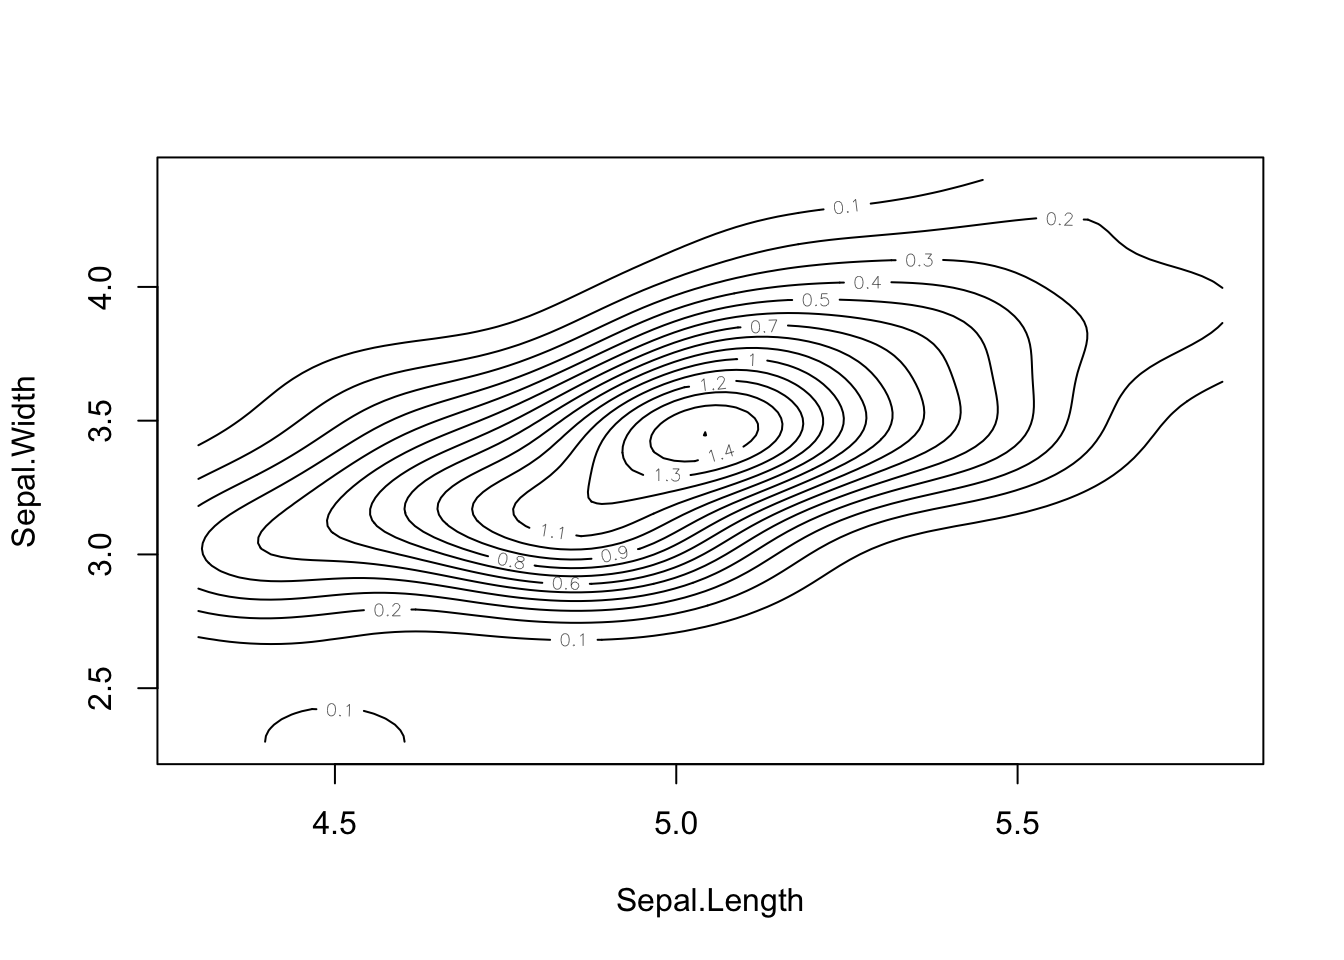
\includegraphics{tsAssignment03_files/figure-latex/unnamed-chunk-12-1.pdf}
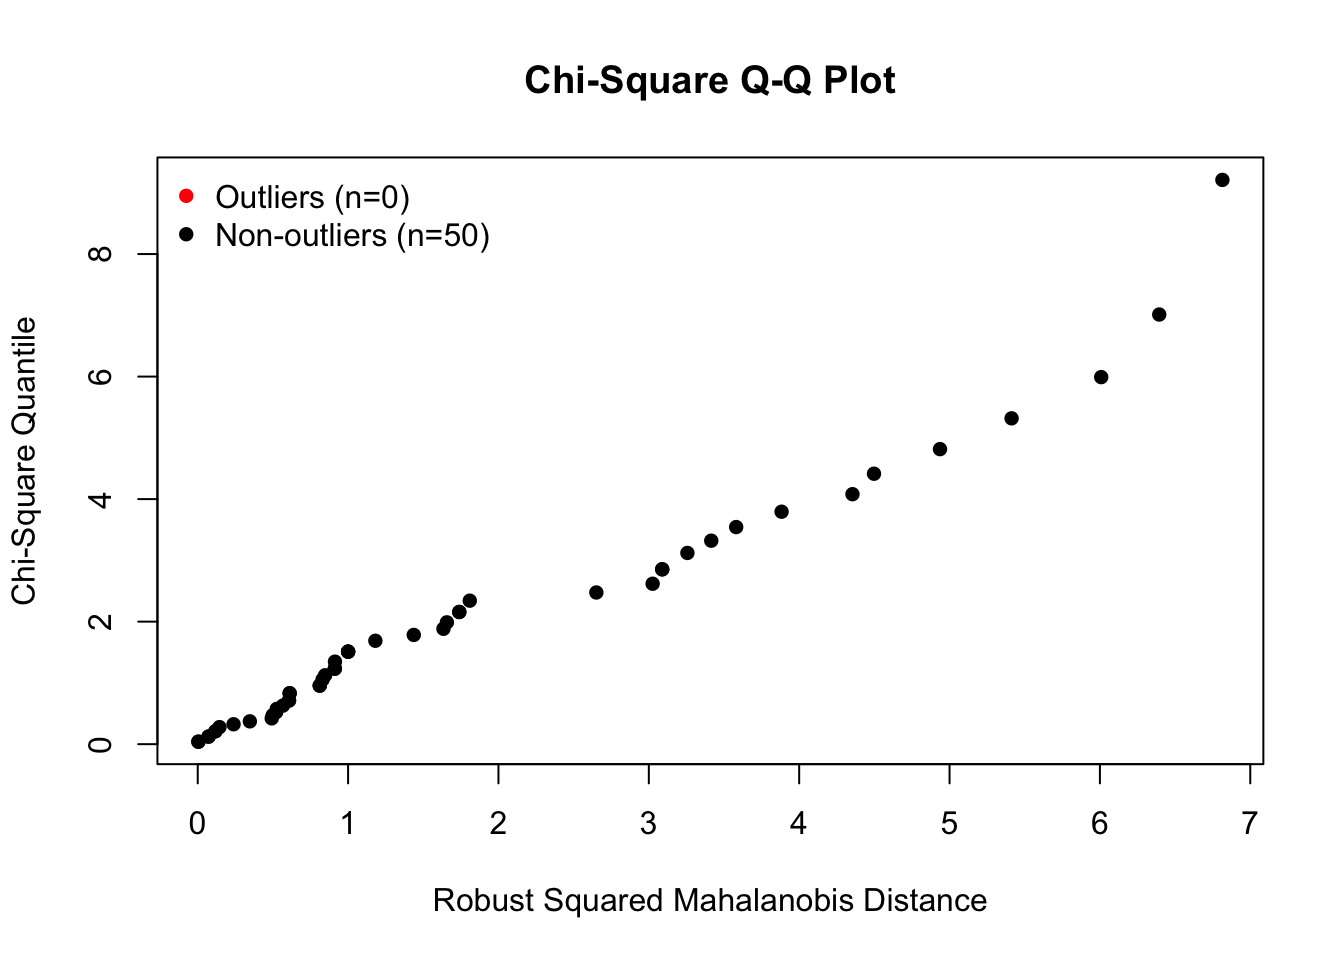
\includegraphics{tsAssignment03_files/figure-latex/unnamed-chunk-12-2.pdf}

\begin{itemize}
\tightlist
\item
  However, it disappears when we take the log of our time series
\end{itemize}

\hypertarget{tests-for-volatility-clustering-in-variance}{%
\subsection{Tests for Volatility Clustering in
Variance}\label{tests-for-volatility-clustering-in-variance}}

\hypertarget{mcleod-li-test}{%
\subsubsection{McLeod Li Test}\label{mcleod-li-test}}

\begin{quote}
ACF, PACF and EACF all shows pattern of white noise for the correlation
structure. However, there is an ARCH effect present in the series.
\end{quote}

\begin{Shaded}
\begin{Highlighting}[]
\NormalTok{doMcleod <-}\StringTok{ }\ControlFlowTok{function}\NormalTok{(df.ts, plotTitle) \{}
  \KeywordTok{doPar}\NormalTok{(}\DataTypeTok{mfrow =} \KeywordTok{c}\NormalTok{(}\DecValTok{1}\NormalTok{, }\DecValTok{1}\NormalTok{))}
  \KeywordTok{McLeod.Li.test}\NormalTok{(}
    \DataTypeTok{y =}\NormalTok{ df.ts,}
    \DataTypeTok{main =}\NormalTok{ plotTitle }
\NormalTok{  )}
\NormalTok{\}}

\KeywordTok{doMcleod}\NormalTok{(data.ts__log_diff1,}
  \DataTypeTok{plotTitle =} \KeywordTok{fig_nums}\NormalTok{(}\StringTok{'McLeod_first_diff'}\NormalTok{, }\StringTok{'McLeod Li Test Second diff'}\NormalTok{)}
\NormalTok{)}
\end{Highlighting}
\end{Shaded}

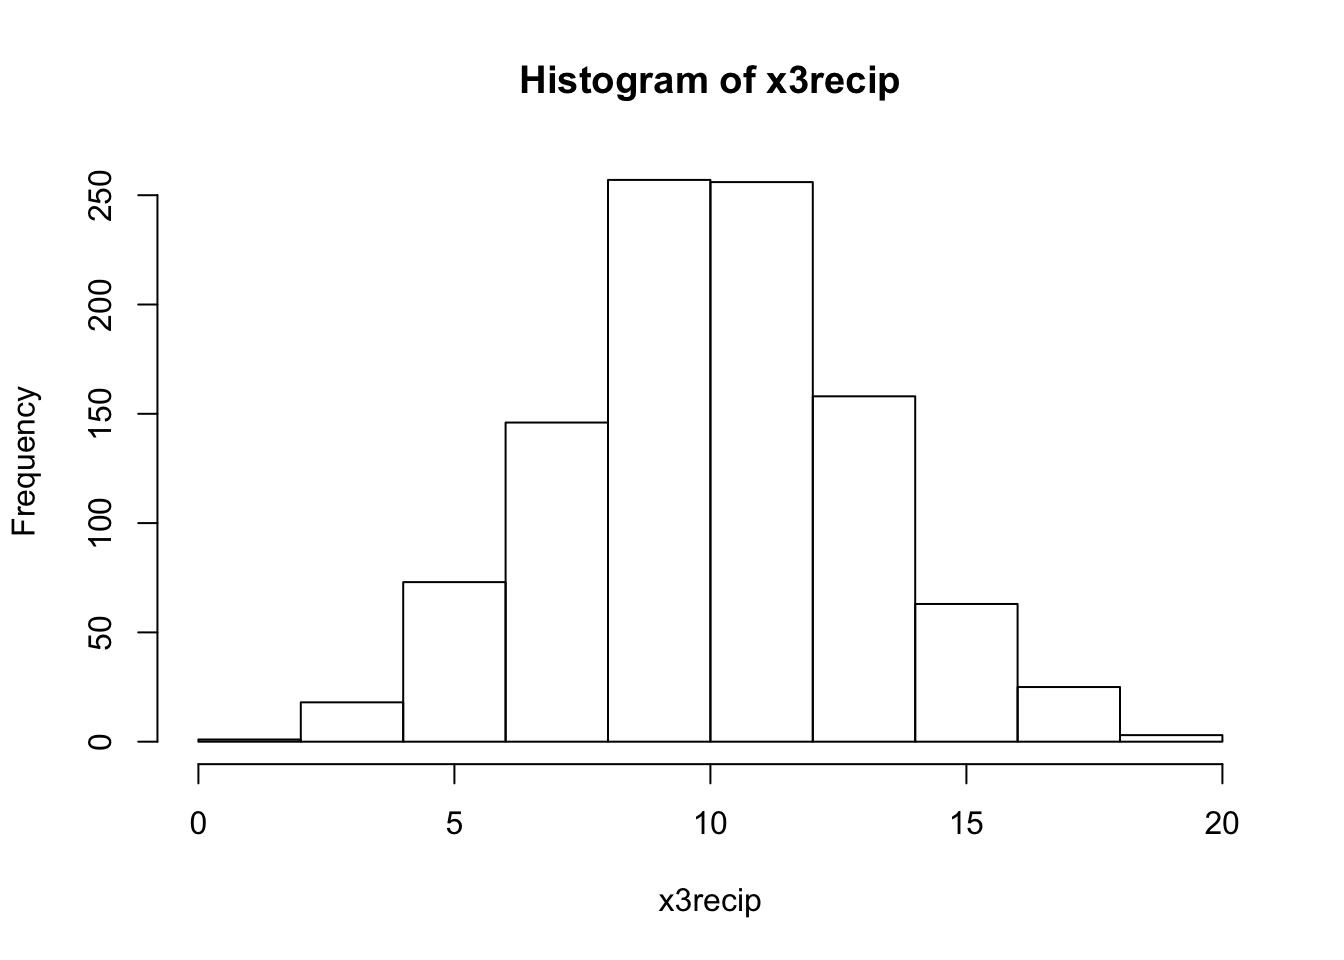
\includegraphics{tsAssignment03_files/figure-latex/unnamed-chunk-13-1.pdf}

\begin{itemize}
\tightlist
\item
  McLeod-Li test is significant at 5\% level of significance for all
  lags for the second diff
\item
  This gives a strong idea about existence of volatility clustering.
\end{itemize}

\hypertarget{q-q-plot}{%
\subsubsection{Q-Q plot}\label{q-q-plot}}

\begin{Shaded}
\begin{Highlighting}[]
\KeywordTok{doPar}\NormalTok{(}\DataTypeTok{mfrow =} \KeywordTok{c}\NormalTok{(}\DecValTok{1}\NormalTok{, }\DecValTok{1}\NormalTok{))}
\KeywordTok{qqnorm}\NormalTok{(}
\NormalTok{  data.ts__log_diff1,}
  \DataTypeTok{main =} \KeywordTok{fig_nums}\NormalTok{(}
    \StringTok{"qq_first_diff_log"}\NormalTok{,}
    \StringTok{"Q-Q Normal Plot of Second Difference of Log Bitcoin"}\NormalTok{)}
\NormalTok{  )}
\KeywordTok{qqline}\NormalTok{(data.ts__log_diff1)}
\end{Highlighting}
\end{Shaded}

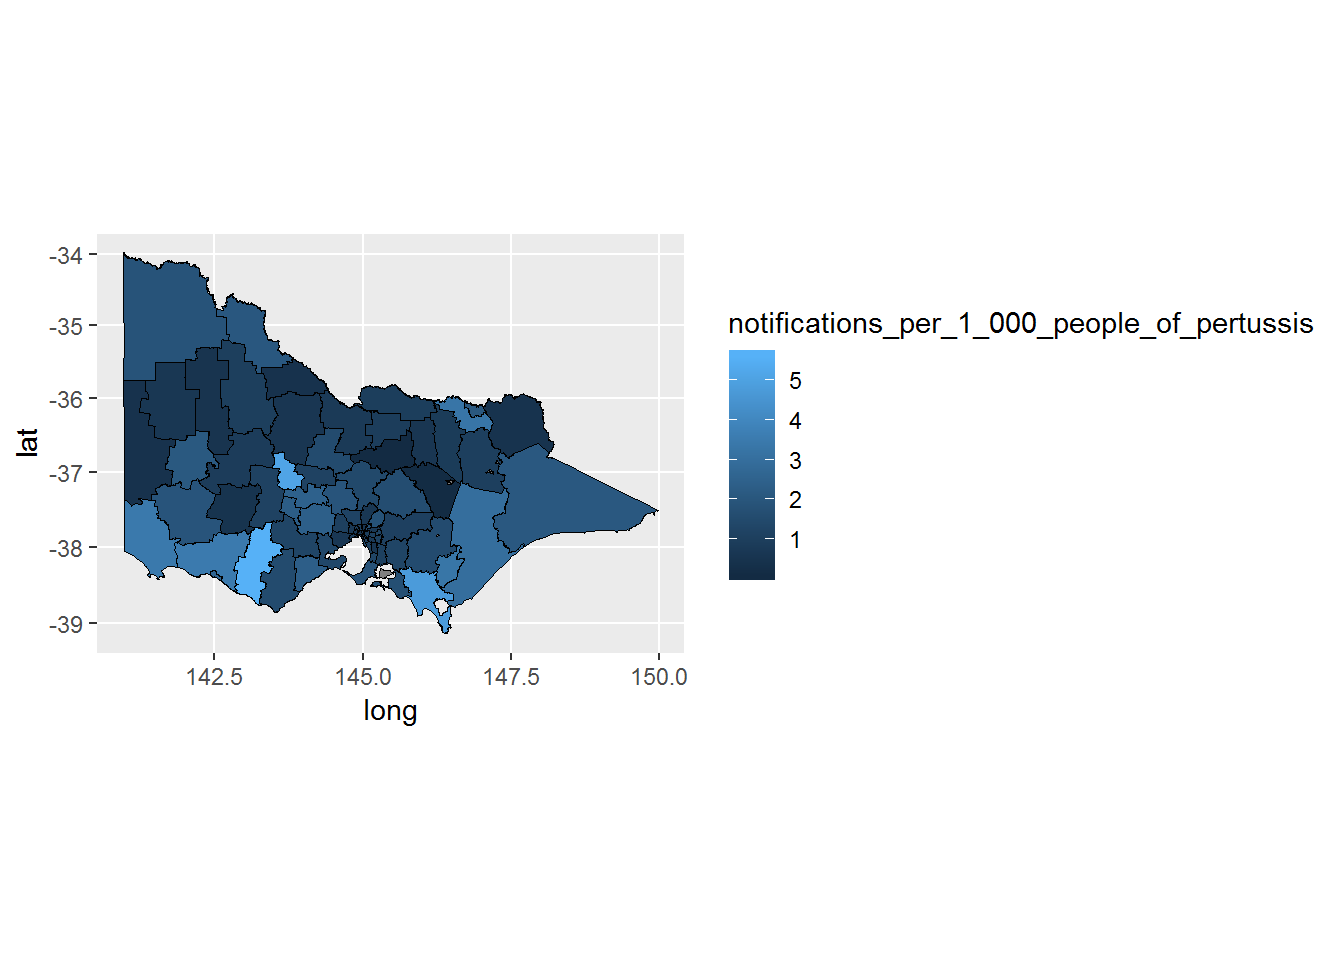
\includegraphics{tsAssignment03_files/figure-latex/unnamed-chunk-14-1.pdf}
- Q-Q plot has a fat tail - Which is also indicative of volatility
clustering

\hypertarget{absolute-value-transformation}{%
\paragraph{Absolute Value
transformation}\label{absolute-value-transformation}}

\begin{Shaded}
\begin{Highlighting}[]
\NormalTok{doAbs <-}\StringTok{ }\ControlFlowTok{function}\NormalTok{(df.ts, plotTitle) \{}
\NormalTok{  abs.df =}\StringTok{ }\KeywordTok{abs}\NormalTok{(df.ts)}
  \KeywordTok{doDiffAndPlot}\NormalTok{(}
    \KeywordTok{abs}\NormalTok{(df.ts), }\DecValTok{0}\NormalTok{, T, F, plotTitle)}
\NormalTok{\}}

\KeywordTok{doAbs}\NormalTok{(}
\NormalTok{  data.ts__log_diff1,}
  \KeywordTok{fig_nums}\NormalTok{(}\StringTok{"absolute_transformation_diff"}\NormalTok{, }\StringTok{"Absolute Transformation diff=1"}\NormalTok{)}
\NormalTok{)}
\end{Highlighting}
\end{Shaded}

\begin{verbatim}
## diff:  0 
## 
## 
## adf p-value: 
## 0.0201489620701211 < 0.05 significant
## 
## AR/MA
##   0 1 2 3 4 5 6 7 8 9 10 11 12 13
## 0 x x x x x x x x x x x  x  x  x 
## 1 x x o o x x o o o x o  o  o  o 
## 2 x x o o o x o o o x o  o  o  o 
## 3 x x x o o o o o o o o  o  o  o 
## 4 x x x x o o o o o o o  o  o  o 
## 5 x x x x x x o o o o o  o  o  o 
## 6 x x x x x o o o o o o  o  o  o 
## 7 x x x x x o o o o o o  o  o  o
\end{verbatim}

\includegraphics{tsAssignment03_files/figure-latex/absolute_transformation-1.pdf}

\begin{itemize}
\item
  We observe many signficant lags in both ACF and PACF.
\item
  EACF does not suggest an ARMA(0,0) model - indicating possible GARCH
  effect
\item
  The EACF does not display a very clear pattern
\item
  Based on EACF plot, we can add the following models:
  \texttt{\{ARIMA(2,1,1),\ ARIMA(2,1,2),\ ARIMA(3,1,1),\ ARIMA(3,1,2)\}}
\item
  We have some evidence that the Bitcoin closing prices are not
  independently and identically distributed, because we observe some
  significant correlations in these plots We will now move on to
  specifying the GARCH parameters
\item
  These models correspond to parameter settings of:

  \begin{itemize}
  \tightlist
  \item
    \texttt{{[}max(2,1),1{]}} =\textgreater{} \texttt{GARCH(2,1)}
  \item
    \texttt{{[}max(2,2),1{]}} =\textgreater{} \texttt{GARCH(2,1)}
  \item
    \texttt{{[}max(3,1),1{]}} =\textgreater{} \texttt{GARCH(3,1)}
  \item
    \texttt{{[}max(3,2),1{]}} =\textgreater{} \texttt{GARCH(3,1)}
  \end{itemize}
\end{itemize}

\begin{Shaded}
\begin{Highlighting}[]
\NormalTok{possibleGarchModels <-}\StringTok{ }\KeywordTok{list}\NormalTok{(}
  \KeywordTok{c}\NormalTok{(}\DecValTok{2}\NormalTok{,}\DecValTok{1}\NormalTok{),}
  \KeywordTok{c}\NormalTok{(}\DecValTok{3}\NormalTok{,}\DecValTok{1}\NormalTok{)}
\NormalTok{)}
\end{Highlighting}
\end{Shaded}

\hypertarget{power-transformation}{%
\paragraph{Power Transformation}\label{power-transformation}}

\begin{Shaded}
\begin{Highlighting}[]
\NormalTok{sq.data.ts__log_diff1 =}\StringTok{ }\NormalTok{data.ts__log_diff1 }\OperatorTok{^}\StringTok{ }\DecValTok{2}
\KeywordTok{doDiffAndPlot}\NormalTok{(}
\NormalTok{  sq.data.ts__log_diff1, }\DecValTok{0}\NormalTok{, T, T, }
  \KeywordTok{fig_nums}\NormalTok{(}\StringTok{'square-transform'}\NormalTok{,}\StringTok{'Square transformation'}\NormalTok{))}
\end{Highlighting}
\end{Shaded}

\begin{verbatim}
## diff:  0
\end{verbatim}

\begin{verbatim}
## Warning in adfTest(df.ts, lags = order, title = NULL, description = NULL):
## p-value smaller than printed p-value
\end{verbatim}

\begin{verbatim}
## 
## adf p-value: 
## 0.01 < 0.05 significant
## 
## AR/MA
##   0 1 2 3 4 5 6 7 8 9 10 11 12 13
## 0 x x x x x x x x x x x  x  x  x 
## 1 x x x x x x o x o x o  o  x  o 
## 2 x x x o o x o o o x o  o  x  o 
## 3 x x x o o x o o o x o  o  x  o 
## 4 x x x o o o o o o o o  o  x  o 
## 5 x x x o x x o o o o o  o  o  o 
## 6 x x x x x x o o o o o  o  o  o 
## 7 x x x x x x x o o o o  o  o  o
\end{verbatim}

\includegraphics{tsAssignment03_files/figure-latex/unnamed-chunk-16-1.pdf}

\begin{itemize}
\item
  We observe many signficant lags in both ACF and PACF.
\item
  EACF does not suggest an ARMA(0,0) model - indicating possible GARCH
  effect
\item
  The EACF does not display a very clear pattern
\item
  Based on EACF plot, we can add the following models:
  \texttt{\{ARIMA(3,1,2),\ ARIMA(4,1,2),\ ARIMA(3,1,3),\ ARIMA(4,1,3),\ ARIMA(4,1,4)}
\item
  We have some evidence that the Bitcoin closing prices are not
  independently and identically distributed, because we observe some
  significant correlations in these plots We will now move on to
  specifying the GARCH parameters
\item
  These models correspond to parameter settings of:

  \begin{itemize}
  \tightlist
  \item
    \texttt{max(3,2),1{]}} =\textgreater{} \texttt{GARCH(3,1)}
  \item
    \texttt{max(4,2),1{]}} =\textgreater{} \texttt{GARCH(4,1)}
  \item
    \texttt{max(3,3),1{]}} =\textgreater{} \texttt{GARCH(3,1)} Repeated
  \item
    \texttt{max(4,3),1{]}} =\textgreater{} \texttt{GARCH(4,1)} Repeated
  \item
    \texttt{max(4,4),1{]}} =\textgreater{} \texttt{GARCH(4,1)} Repeated
  \end{itemize}
\end{itemize}

The possible candidate GARCH models are:

\begin{itemize}
\tightlist
\item
  \texttt{GARCH(2,1)}
\item
  \texttt{GARCH(3,1)}
\item
  \texttt{GARCH(4,1)}
\end{itemize}

\begin{Shaded}
\begin{Highlighting}[]
\NormalTok{  newGarch <-}
\StringTok{    }\KeywordTok{list}\NormalTok{(  }
      \KeywordTok{c}\NormalTok{(}\DecValTok{4}\NormalTok{, }\DecValTok{1}\NormalTok{)   }\CommentTok{# arima(1, 1, 2)}
\NormalTok{    )}
\NormalTok{  possibleGarchModels <-}\StringTok{ }\KeywordTok{c}\NormalTok{(possibleGarchModels, newGarch) }
\end{Highlighting}
\end{Shaded}

\hypertarget{garch-parameter-estimations}{%
\subsubsection{Garch Parameter
Estimations}\label{garch-parameter-estimations}}

\begin{Shaded}
\begin{Highlighting}[]
\NormalTok{possibleGarchModels}
\end{Highlighting}
\end{Shaded}

\begin{verbatim}
## [[1]]
## [1] 2 1
## 
## [[2]]
## [1] 3 1
## 
## [[3]]
## [1] 4 1
\end{verbatim}

\begin{Shaded}
\begin{Highlighting}[]
\NormalTok{g21 =}\StringTok{ }\KeywordTok{garch}\NormalTok{( data.ts__log_diff1, }\DataTypeTok{order =} \KeywordTok{c}\NormalTok{(}\DecValTok{2}\NormalTok{,}\DecValTok{1}\NormalTok{),}\DataTypeTok{trace =} \OtherTok{FALSE}\NormalTok{)}
\KeywordTok{summary}\NormalTok{(g21)}
\end{Highlighting}
\end{Shaded}

\begin{verbatim}
## 
## Call:
## garch(x = data.ts__log_diff1, order = c(2, 1), trace = FALSE)
## 
## Model:
## GARCH(2,1)
## 
## Residuals:
##      Min       1Q   Median       3Q      Max 
## -8.39959 -0.36388  0.05552  0.50988  4.73268 
## 
## Coefficient(s):
##     Estimate  Std. Error  t value Pr(>|t|)    
## a0 5.656e-05   5.011e-06   11.287  < 2e-16 ***
## a1 1.789e-01   1.157e-02   15.460  < 2e-16 ***
## b1 2.244e-01   4.622e-02    4.855  1.2e-06 ***
## b2 5.794e-01   4.146e-02   13.973  < 2e-16 ***
## ---
## Signif. codes:  0 '***' 0.001 '**' 0.01 '*' 0.05 '.' 0.1 ' ' 1
## 
## Diagnostic Tests:
##  Jarque Bera Test
## 
## data:  Residuals
## X-squared = 5021.2, df = 2, p-value < 2.2e-16
## 
## 
##  Box-Ljung test
## 
## data:  Squared.Residuals
## X-squared = 0.061721, df = 1, p-value = 0.8038
\end{verbatim}

\begin{itemize}
\tightlist
\item
  Looks good. Significant at all Coef.
\end{itemize}

\begin{Shaded}
\begin{Highlighting}[]
\NormalTok{g31 =}\StringTok{ }\KeywordTok{garch}\NormalTok{( data.ts__log_diff1, }\DataTypeTok{order =} \KeywordTok{c}\NormalTok{(}\DecValTok{3}\NormalTok{,}\DecValTok{1}\NormalTok{),}\DataTypeTok{trace =} \OtherTok{FALSE}\NormalTok{)}
\KeywordTok{summary}\NormalTok{(g31)}
\end{Highlighting}
\end{Shaded}

\begin{verbatim}
## 
## Call:
## garch(x = data.ts__log_diff1, order = c(3, 1), trace = FALSE)
## 
## Model:
## GARCH(3,1)
## 
## Residuals:
##     Min      1Q  Median      3Q     Max 
## -8.3567 -0.3605  0.0567  0.5055  4.6630 
## 
## Coefficient(s):
##     Estimate  Std. Error  t value Pr(>|t|)    
## a0 6.856e-05   7.806e-06    8.783  < 2e-16 ***
## a1 2.082e-01   2.083e-02    9.997  < 2e-16 ***
## b1 3.398e-01   8.276e-02    4.106 4.02e-05 ***
## b2 4.379e-01   7.642e-02    5.731 1.00e-08 ***
## b3 1.401e-08   7.256e-02    0.000        1    
## ---
## Signif. codes:  0 '***' 0.001 '**' 0.01 '*' 0.05 '.' 0.1 ' ' 1
## 
## Diagnostic Tests:
##  Jarque Bera Test
## 
## data:  Residuals
## X-squared = 5622.7, df = 2, p-value < 2.2e-16
## 
## 
##  Box-Ljung test
## 
## data:  Squared.Residuals
## X-squared = 0.013398, df = 1, p-value = 0.9079
\end{verbatim}

\begin{itemize}
\tightlist
\item
  Looks good. Significant at all Coef.
\end{itemize}

\begin{Shaded}
\begin{Highlighting}[]
\NormalTok{g41 =}\StringTok{ }\KeywordTok{garch}\NormalTok{( data.ts__log_diff1, }\DataTypeTok{order =} \KeywordTok{c}\NormalTok{(}\DecValTok{4}\NormalTok{,}\DecValTok{1}\NormalTok{),}\DataTypeTok{trace =} \OtherTok{FALSE}\NormalTok{)}
\KeywordTok{summary}\NormalTok{(g41)}
\end{Highlighting}
\end{Shaded}

\begin{verbatim}
## 
## Call:
## garch(x = data.ts__log_diff1, order = c(4, 1), trace = FALSE)
## 
## Model:
## GARCH(4,1)
## 
## Residuals:
##      Min       1Q   Median       3Q      Max 
## -8.25619 -0.36246  0.05676  0.49612  5.04342 
## 
## Coefficient(s):
##     Estimate  Std. Error  t value Pr(>|t|)    
## a0 6.451e-05   5.808e-06   11.108  < 2e-16 ***
## a1 2.303e-01   1.411e-02   16.314  < 2e-16 ***
## b1 3.523e-01   5.970e-02    5.901  3.6e-09 ***
## b2 2.390e-02   5.669e-02    0.422    0.673    
## b3 3.161e-09   5.228e-02    0.000    1.000    
## b4 3.802e-01   3.361e-02   11.312  < 2e-16 ***
## ---
## Signif. codes:  0 '***' 0.001 '**' 0.01 '*' 0.05 '.' 0.1 ' ' 1
## 
## Diagnostic Tests:
##  Jarque Bera Test
## 
## data:  Residuals
## X-squared = 5256.6, df = 2, p-value < 2.2e-16
## 
## 
##  Box-Ljung test
## 
## data:  Squared.Residuals
## X-squared = 0.10997, df = 1, p-value = 0.7402
\end{verbatim}

\begin{itemize}
\tightlist
\item
  Significant at all except \texttt{b2} and \texttt{b3}
\item
  Discarded
\end{itemize}

\begin{Shaded}
\begin{Highlighting}[]
\CommentTok{# hidden:}
\CommentTok{# g41 = garch( data.ts__log_diff1, order = c(4,1),trace = FALSE)}
\CommentTok{# summary(g41)}
\end{Highlighting}
\end{Shaded}

\begin{itemize}
\tightlist
\item
  significant at all bar \texttt{b2}and \texttt{b3}
\end{itemize}

\begin{Shaded}
\begin{Highlighting}[]
\NormalTok{model_s_garch <-}\StringTok{ }\KeywordTok{ugarchspec}\NormalTok{(}
  \DataTypeTok{variance.model =} \KeywordTok{list}\NormalTok{(}\DataTypeTok{model =} \StringTok{"sGARCH"}\NormalTok{, }\DataTypeTok{garchOrder =} \KeywordTok{c}\NormalTok{(}\DecValTok{3}\NormalTok{, }\DecValTok{1}\NormalTok{)),}
  \DataTypeTok{mean.model =} \KeywordTok{list}\NormalTok{(}\DataTypeTok{armaOrder =} \KeywordTok{c}\NormalTok{(}\DecValTok{2}\NormalTok{, }\DecValTok{2}\NormalTok{), }\DataTypeTok{include.mean =} \OtherTok{FALSE}\NormalTok{),}
  \DataTypeTok{distribution.model =} \StringTok{"norm"}
\NormalTok{)}
\NormalTok{model =}\StringTok{ }\KeywordTok{ugarchfit}\NormalTok{(}\DataTypeTok{spec =}\NormalTok{ model_s_garch, }\DataTypeTok{data =}\NormalTok{ data.ts__log_diff1)}

\CommentTok{# }\AlertTok{FIXME}\CommentTok{: working on}
\CommentTok{# exp(diffinv(forc@forecast[["seriesFor"]], differences = 2, xi = log(data.ts)[length(data.ts)]))}
\end{Highlighting}
\end{Shaded}

\hypertarget{residuals-for-arma-garch}{%
\subsubsection{Residuals for
ARMA-GARCH}\label{residuals-for-arma-garch}}

\begin{Shaded}
\begin{Highlighting}[]
\NormalTok{res =}\StringTok{ }\NormalTok{model}\OperatorTok{@}\NormalTok{fit[[}\StringTok{"residuals"}\NormalTok{]]}

\KeywordTok{residual.analysis}\NormalTok{(model, }\DataTypeTok{class =} \StringTok{"ARMA-GARCH"}\NormalTok{)}
\end{Highlighting}
\end{Shaded}

\begin{verbatim}
## 
##  Shapiro-Wilk normality test
## 
## data:  res.model
## W = 0.88566, p-value < 2.2e-16
\end{verbatim}

\includegraphics{tsAssignment03_files/figure-latex/unnamed-chunk-23-1.pdf}

\begin{itemize}
\tightlist
\item
  Time-series standardised residuals:
\item
  histogram:
\item
  Ljung-Box test:
\item
  Q-Q plot:
\item
  ACF:
\item
  Shapiro-Wilk:
\end{itemize}

\hypertarget{arma-garch-forecast}{%
\subsubsection{ARMA-GARCH forecast}\label{arma-garch-forecast}}

\begin{Shaded}
\begin{Highlighting}[]
\NormalTok{forc =}\StringTok{ }\KeywordTok{ugarchforecast}\NormalTok{(model, }\DataTypeTok{n.ahead =} \DecValTok{10}\NormalTok{)}
\NormalTok{forc}\OperatorTok{@}\NormalTok{model}\OperatorTok{$}\NormalTok{modeldata}\OperatorTok{$}\NormalTok{index <-}\StringTok{ }\KeywordTok{seq}\NormalTok{(}\KeywordTok{as.Date}\NormalTok{(}\StringTok{'2013-04-27'}\NormalTok{),}\KeywordTok{as.Date}\NormalTok{(}\StringTok{'2019-02-24'}\NormalTok{),}\DataTypeTok{by =} \DecValTok{1}\NormalTok{)}

\NormalTok{garch_predict =}\StringTok{ }
\StringTok{  }\KeywordTok{ts}\NormalTok{(}
    \KeywordTok{as.vector}\NormalTok{(forc}\OperatorTok{@}\NormalTok{forecast[[}\StringTok{"seriesFor"}\NormalTok{]]), }
    \DataTypeTok{start =} \KeywordTok{c}\NormalTok{(}\DecValTok{2019}\NormalTok{, }\KeywordTok{as.numeric}\NormalTok{(}\KeywordTok{format}\NormalTok{(inds[}\DecValTok{1}\NormalTok{], }\StringTok{"%j"}\NormalTok{))), }
    \DataTypeTok{frequency =} \FloatTok{365.25}
\NormalTok{  )}

\KeywordTok{plot}\NormalTok{(garch_predict)}
\end{Highlighting}
\end{Shaded}

\includegraphics{tsAssignment03_files/figure-latex/unnamed-chunk-24-1.pdf}

\begin{Shaded}
\begin{Highlighting}[]
\NormalTok{garch_predict}
\end{Highlighting}
\end{Shaded}

\begin{verbatim}
## Time Series:
## Start = 2019.31759069131 
## End = 2019.34223134839 
## Frequency = 365.25 
##  [1] -1.320670e-03 -4.259843e-04 -1.382556e-04 -4.563965e-05 -1.575287e-05
##  [6] -6.040927e-06 -2.824171e-06 -1.704441e-06 -1.267106e-06 -1.056641e-06
\end{verbatim}

\begin{Shaded}
\begin{Highlighting}[]
\NormalTok{garch_predict_transform <-}\StringTok{  }\KeywordTok{exp}\NormalTok{(}\KeywordTok{diffinv}\NormalTok{(garch_predict, }\DataTypeTok{differences =} \DecValTok{1}\NormalTok{,  }\DataTypeTok{xi =}\NormalTok{ (data.ts__log)[}\DecValTok{2130}\NormalTok{]))}

\KeywordTok{plot}\NormalTok{(garch_predict_transform)}
\end{Highlighting}
\end{Shaded}

\includegraphics{tsAssignment03_files/figure-latex/unnamed-chunk-24-2.pdf}

\begin{Shaded}
\begin{Highlighting}[]
\KeywordTok{plot}\NormalTok{(data.ts)}
\KeywordTok{lines}\NormalTok{(real.ts, }\DataTypeTok{col =} \StringTok{"#009999"}\NormalTok{)}
\KeywordTok{lines}\NormalTok{(linear_predict, }\DataTypeTok{col=}\StringTok{"red"}\NormalTok{, }\DataTypeTok{type=}\StringTok{"l"}\NormalTok{)}
\KeywordTok{lines}\NormalTok{(quadratic_predict, }\DataTypeTok{col =} \StringTok{"darkgreen"}\NormalTok{, }\DataTypeTok{type =} \StringTok{"l"}\NormalTok{)}
\KeywordTok{lines}\NormalTok{(garch_predict_transform, }\DataTypeTok{col =} \StringTok{"#993333"}\NormalTok{, }\DataTypeTok{type =} \StringTok{"l"}\NormalTok{)}
\end{Highlighting}
\end{Shaded}

\includegraphics{tsAssignment03_files/figure-latex/unnamed-chunk-25-1.pdf}

\begin{Shaded}
\begin{Highlighting}[]
\KeywordTok{zoomplot.zoom}\NormalTok{(}\DataTypeTok{xlim=}\KeywordTok{c}\NormalTok{(}\FloatTok{2018.5}\NormalTok{,}\FloatTok{2019.5}\NormalTok{))}
\end{Highlighting}
\end{Shaded}

\includegraphics{tsAssignment03_files/figure-latex/unnamed-chunk-25-2.pdf}

\begin{Shaded}
\begin{Highlighting}[]
\CommentTok{# Reversing the differencing created an extra datapoint; }
\CommentTok{# we can calculate MASE using first 10 or last 10}
\KeywordTok{MASE}\NormalTok{(real.ts, garch_predict_transform[}\DecValTok{2}\OperatorTok{:}\DecValTok{11}\NormalTok{])}
\end{Highlighting}
\end{Shaded}

\begin{verbatim}
## $MASE
##       MASE
## 1 1.939003
\end{verbatim}

\begin{Shaded}
\begin{Highlighting}[]
\KeywordTok{MASE}\NormalTok{(real.ts, garch_predict_transform[}\DecValTok{1}\OperatorTok{:}\DecValTok{10}\NormalTok{])}
\end{Highlighting}
\end{Shaded}

\begin{verbatim}
## $MASE
##       MASE
## 1 1.915918
\end{verbatim}

\begin{itemize}
\tightlist
\item
  TODO: interpret forecast
\end{itemize}

\hypertarget{todo-conclusion}{%
\subsection{TODO: Conclusion}\label{todo-conclusion}}

The results of the above tests summarised:

TODO: interpret

\begin{Shaded}
\begin{Highlighting}[]
\CommentTok{# outputting plots}
\NormalTok{plots.dir.path <-}
\StringTok{  }\KeywordTok{list.files}\NormalTok{(}
     \KeywordTok{tempdir}\NormalTok{(), }\DataTypeTok{pattern=}\StringTok{"rs-graphics"}\NormalTok{, }\DataTypeTok{full.names =} \OtherTok{TRUE}\NormalTok{);}
\NormalTok{plots.png.paths <-}
\StringTok{ }\KeywordTok{list.files}\NormalTok{(}
\NormalTok{   plots.dir.path, }\DataTypeTok{pattern=}\StringTok{".png"}\NormalTok{, }\DataTypeTok{full.names =} \OtherTok{TRUE}\NormalTok{)}
\end{Highlighting}
\end{Shaded}

\begin{Shaded}
\begin{Highlighting}[]
\KeywordTok{file.copy}\NormalTok{(}
  \DataTypeTok{from=}\NormalTok{plots.png.paths,}
  \DataTypeTok{to=}\StringTok{"~/code/data-science/uni/time-series/assignment03/presentation-ts-assignment03/assets"}\NormalTok{)}
\end{Highlighting}
\end{Shaded}

\begin{verbatim}
## logical(0)
\end{verbatim}


\end{document}
